\documentclass[11pt]{article}

\usepackage[margin=1in]{geometry}
\usepackage{setspace}
\onehalfspacing
\usepackage{graphicx}
\graphicspath{report_images/}
\usepackage{appendix}
\usepackage{listings}
\usepackage{float}
\usepackage{multirow}
\usepackage{amsthm}
% The next three lines make the table and figure numbers also include section number
\usepackage{chngcntr}
\counterwithin{table}{section}
\counterwithin{figure}{section}
% Needed to make titling page without a page number
\usepackage{titling}

% DOCUMENT INFORMATION =================================================
\font\titleFont=cmr12 at 11pt
\title {{\titleFont ECEN 429: Introduction to Digital Systems Design Laboratory \\ North Carolina Agricultural and Technical State University \\ Department of Electrical and Computer Engineering}} % Declare Title
\author{\titleFont Reporter: Nikiyah Beulah \\ \titleFont Partner: Chris Cannon} % Declare authors
\date{\titleFont February 15, 2018}
% ======================================================================

\begin{document}

\begin{titlingpage}
\maketitle
\begin{center}
	Lab 4
\end{center}
\end{titlingpage}

\section{Introduction}
The object of this lab is to introduce students to the topic of memory and show how we might represent and handle memory in VHDL. This lab also reiterated important important concepts about components that will be utilized in this project. By the end of this lab, we will be able to implement a basic memory module in VHDL with the ability to select specific values from the memory address.

\section{Background, Design Solution, and Results}

\subsection{Problem 1 ROM Implementation}

\subsubsection{Background}
We were instructed to implement a ROM module with a 4-bit input and a 3-bit output. Because there are 4-inputs, which correspond with the available addresses in this memory. 4-bits corresponds with 2\textsuperscript{4}, or 16 possible values. Therefore, we were able to derive that there are 16 addresses in this memory module. Because the output is only 3 bits, we knew that our memory word size was 3 bits, meaning that each memory address held 3 bits of data.

\subsubsection{Design Solution}

The design we came up with for this ROM is a simple case statement what will retrieve a different value for each address. To populate our ROM for testing purposes, we decided to simply start with output "000" and iterate to "111", twice. It should be noted that the output values are trivial in this assignment. The point is to return a value stored at a given address, but the actual data stored there does not matter for this assignment. Students attempting to recreate this lab are encouraged to come up with their own values for output if they wish. The truth table for the ROM is shown in Table ~\ref{tab:romTruthTable} and the port assignments are summarized in Table ~\ref{tab:romPorts}.

\begin{table}[H]
\begin{center}
\begin{tabular}{| l | l | l | l | l |}
	\hline
	a3 & a2 & a1 & a0 & output \\ \hline
	0 & 0 & 0 & 0 & 000 \\ \hline
	0 & 0 & 0 & 1 & 001 \\ \hline
	0 & 0 & 1 & 0 & 010 \\ \hline
	0 & 0 & 1 & 1 & 011 \\ \hline
	0 & 1 & 0 & 0 & 100 \\ \hline
	0 & 1 & 0 & 1 & 101 \\ \hline
	0 & 1 & 1 & 0 & 110 \\ \hline
	0 & 1 & 1 & 1 & 111 \\ \hline
	1 & 0 & 0 & 0 & 000 \\ \hline
	1 & 0 & 0 & 1 & 001 \\ \hline
	1 & 0 & 1 & 0 & 010 \\ \hline
	1 & 0 & 1 & 1 & 011 \\ \hline
	1 & 1 & 0 & 0 & 100 \\ \hline
	1 & 1 & 0 & 1 & 101 \\ \hline
	1 & 1 & 1 & 0 & 110 \\ \hline
	1 & 1 & 1 & 1 & 111 \\ \hline
\end{tabular}
\caption{\label{tab:romTruthTable}Truth table for our ROM implementation.}
\end{center}
\end{table}

\begin{table}[H]
\begin{center}
\begin{tabular}{| l | l | l |}
	\hline
	Bit & Label & Port \\ \hline
	a3 & Switch 3 & W17 \\ \hline
	a2 & Switch 2 & W16 \\ \hline
	a1 & Switch 1 & V16 \\ \hline
	a0 & Switch 0 & V17 \\ \hline
	o2 & LED 2 & U19 \\ \hline
	o1 & LED 1 & E19 \\ \hline
	o0 & LED 0 & U16 \\ \hline
\end{tabular}
\caption{\label{tab:romPorts}Port assignments for ROM implementation.}
\end{center}
\end{table}

\subsubsection{Results}
The ROM was successfully implemented and tested on our Basys3 board. We were able to successfully demonstrate returning every value specified in our truth table. Figures ~\ref{fig:p1img1} through ~\ref{fig:p1img9} show a sample of our results for chosen inputs.

\begin{figure}[H]
\begin{center}
	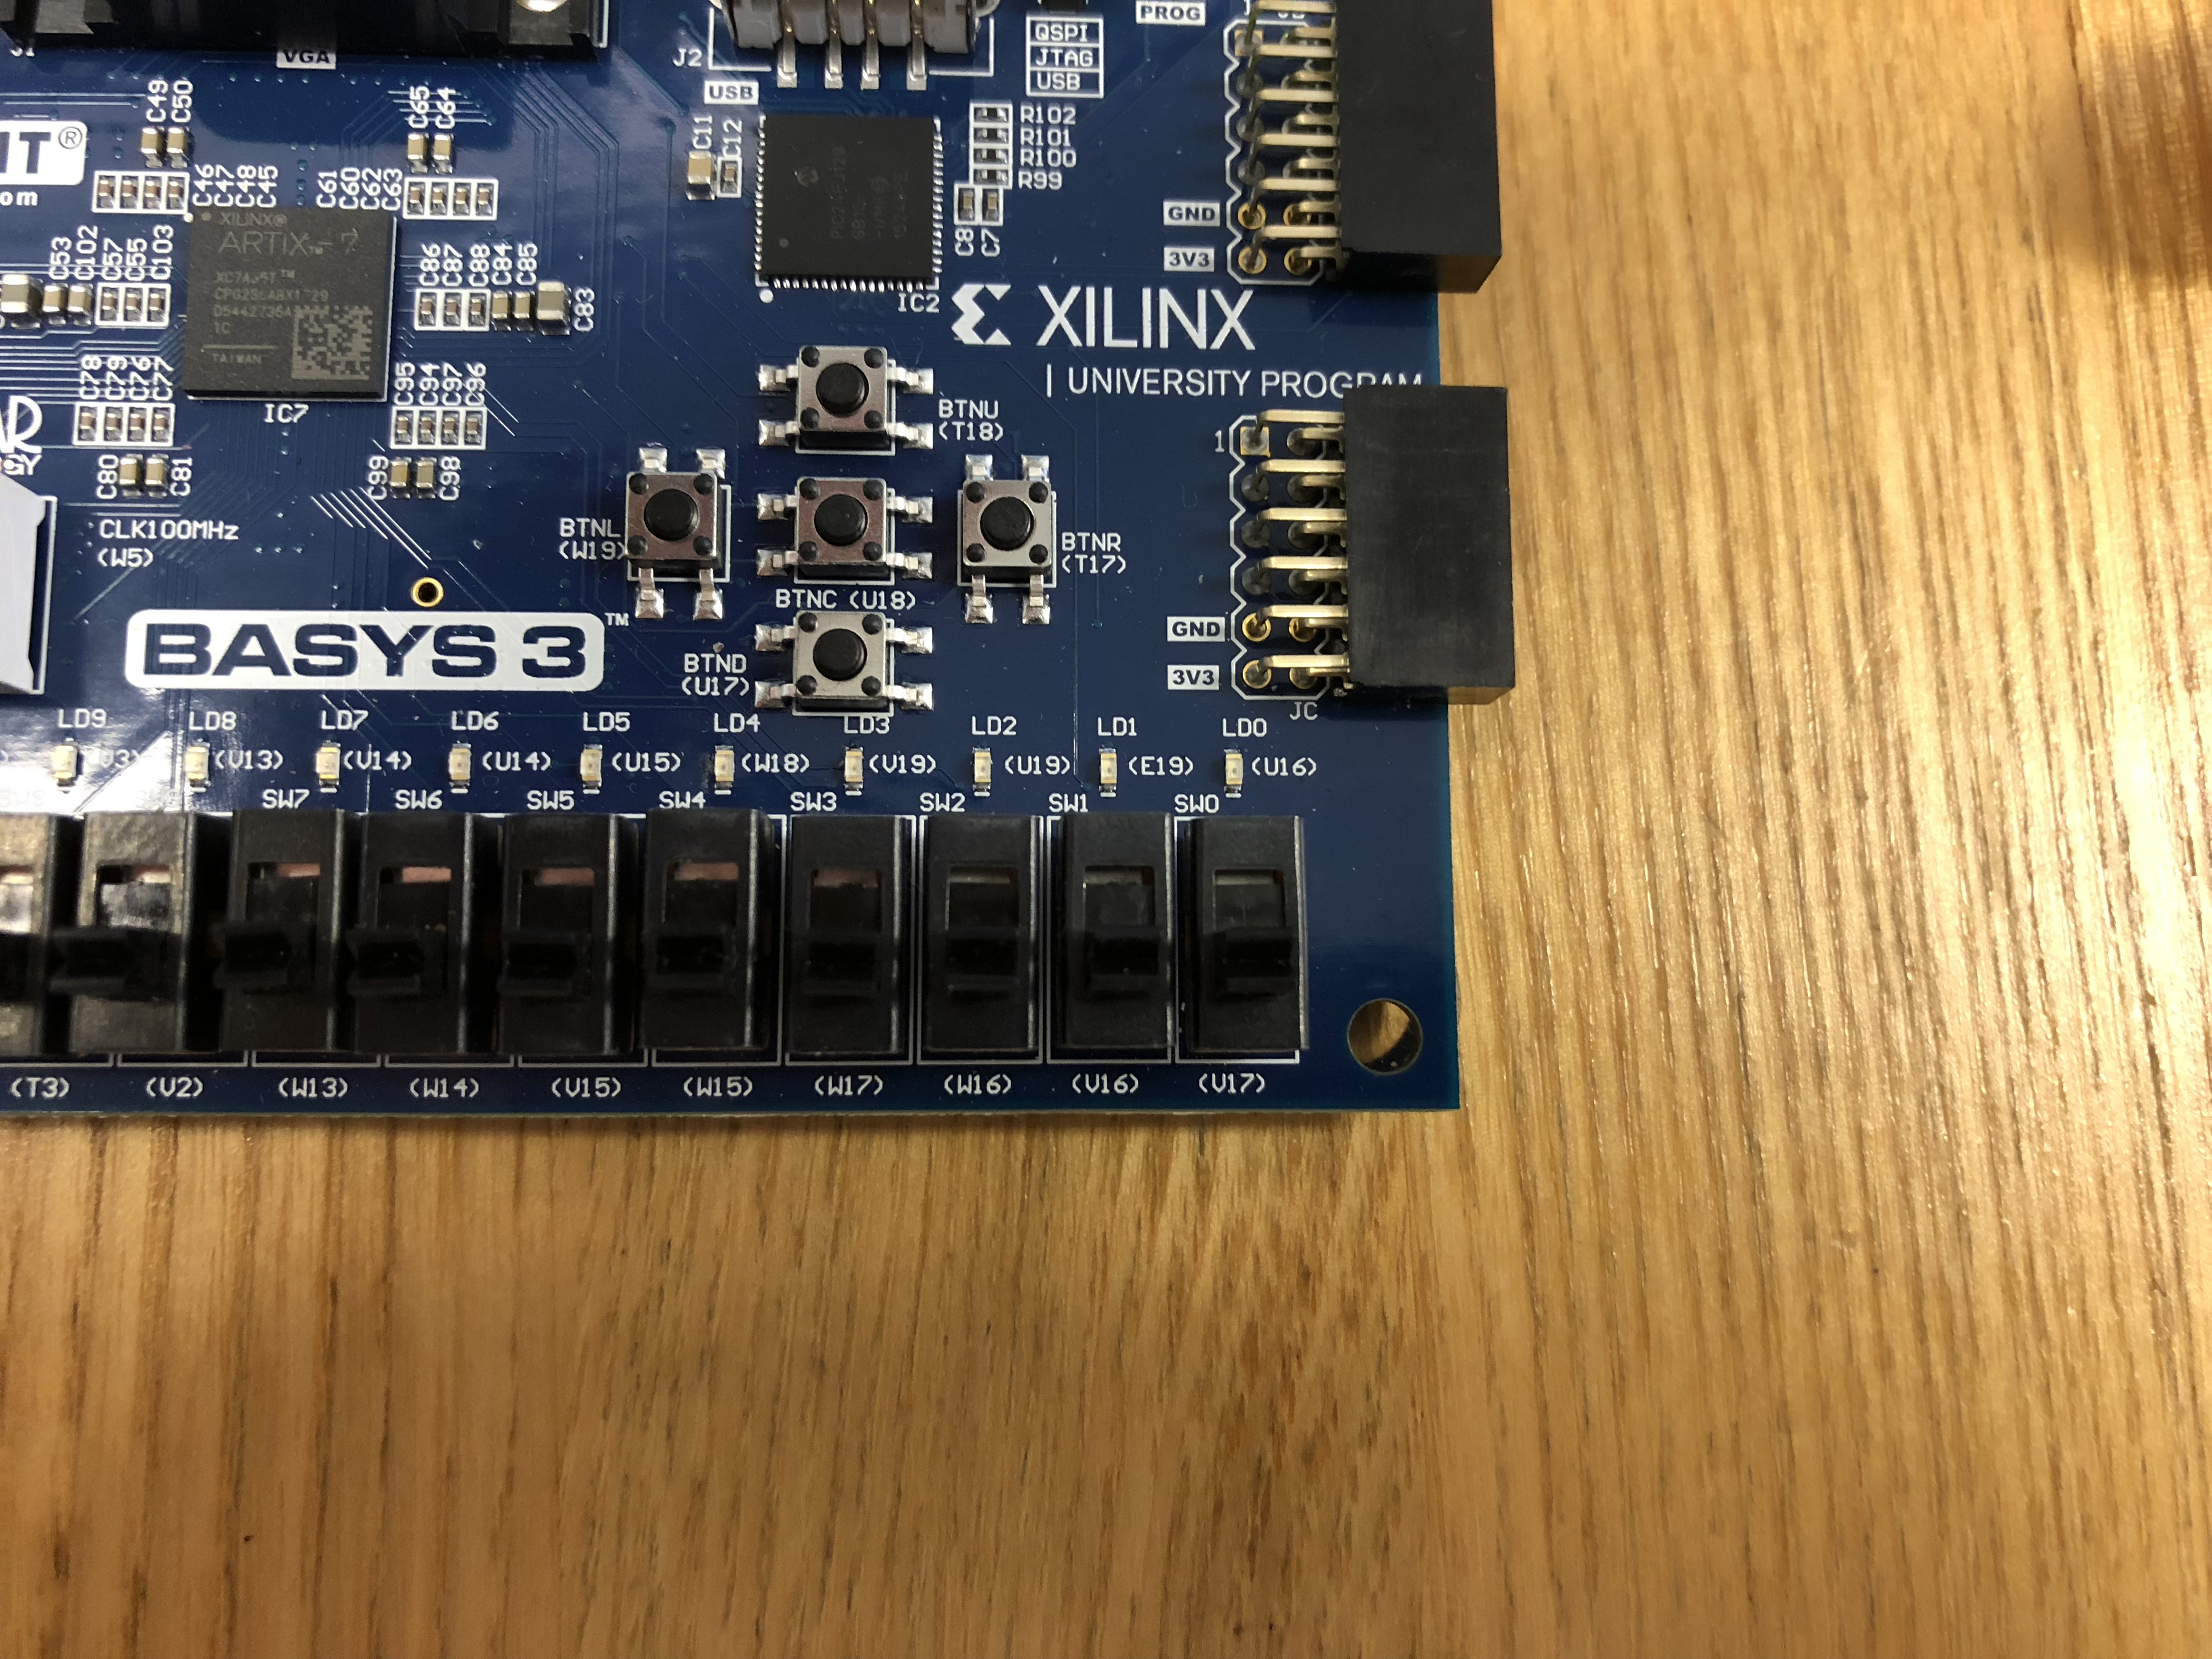
\includegraphics[width=0.5\textwidth]{../report-images/Part1/IMG_3076.jpg}
	\caption{\label{fig:p1img1}The input given by the switches is "0000" and the output shown by the LEDs is "000".}
\end{center}
\end{figure}

\begin{figure}[H]
\begin{center}
	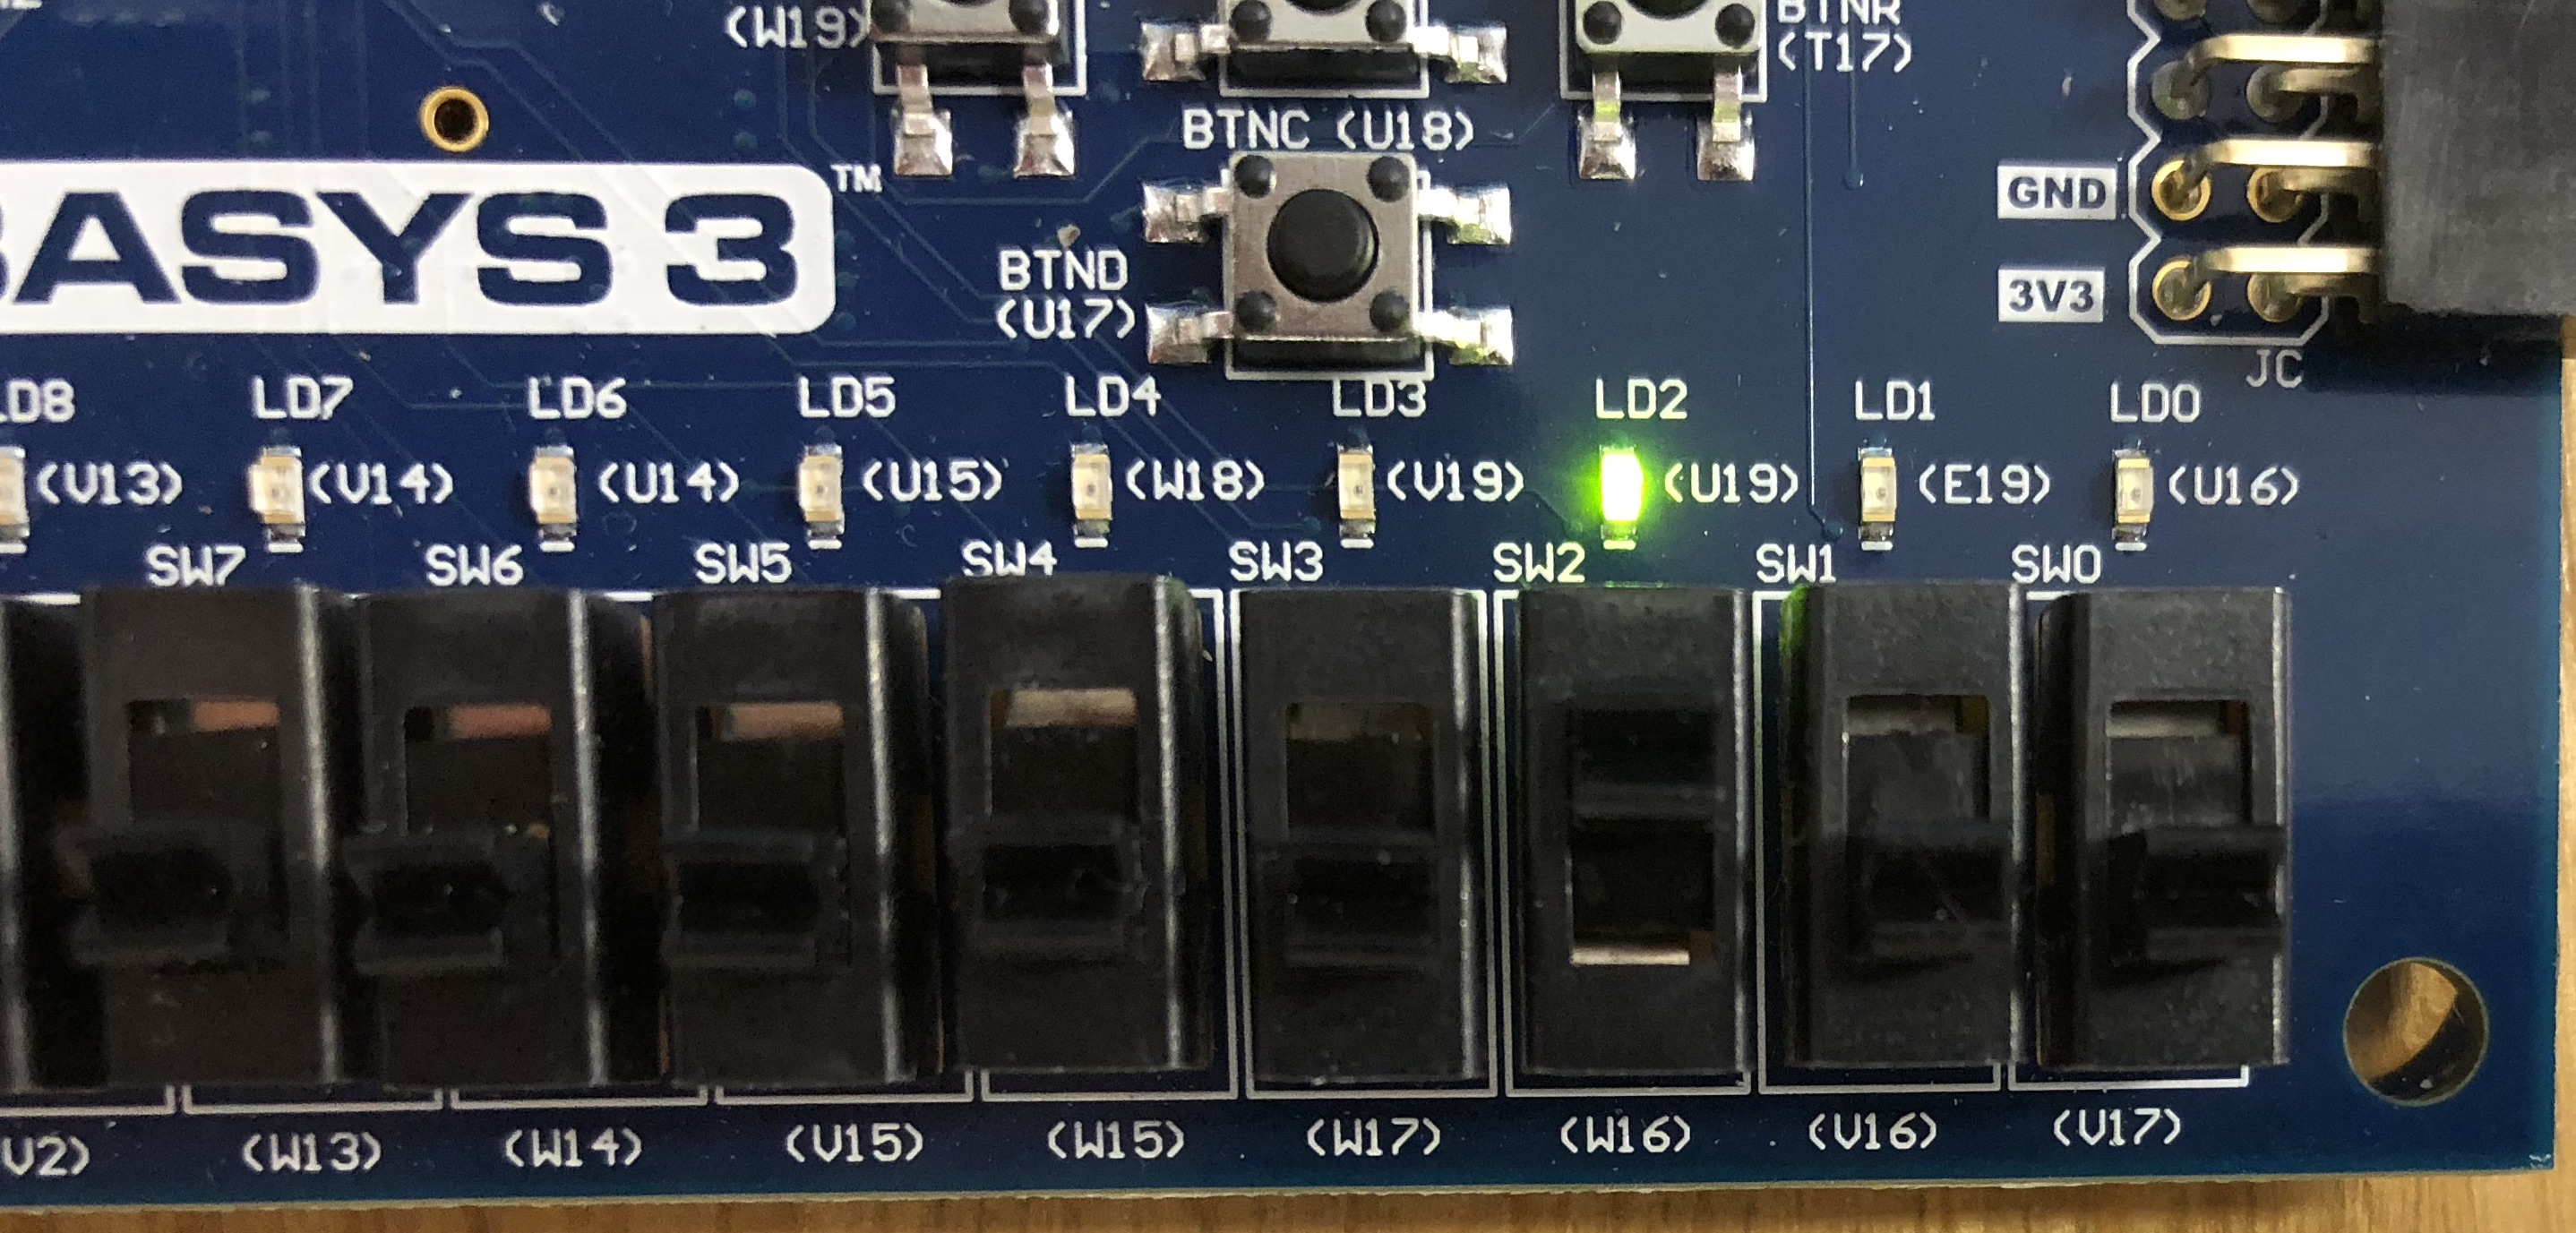
\includegraphics[width=0.5\textwidth]{../report-images/Part1/IMG_3081.jpg}
	\caption{\label{fig:p1img2}The input given by the switches is "0100" and the output shown by the LEDs is "100".}
\end{center}
\end{figure}

\begin{figure}[H]
\begin{center}
	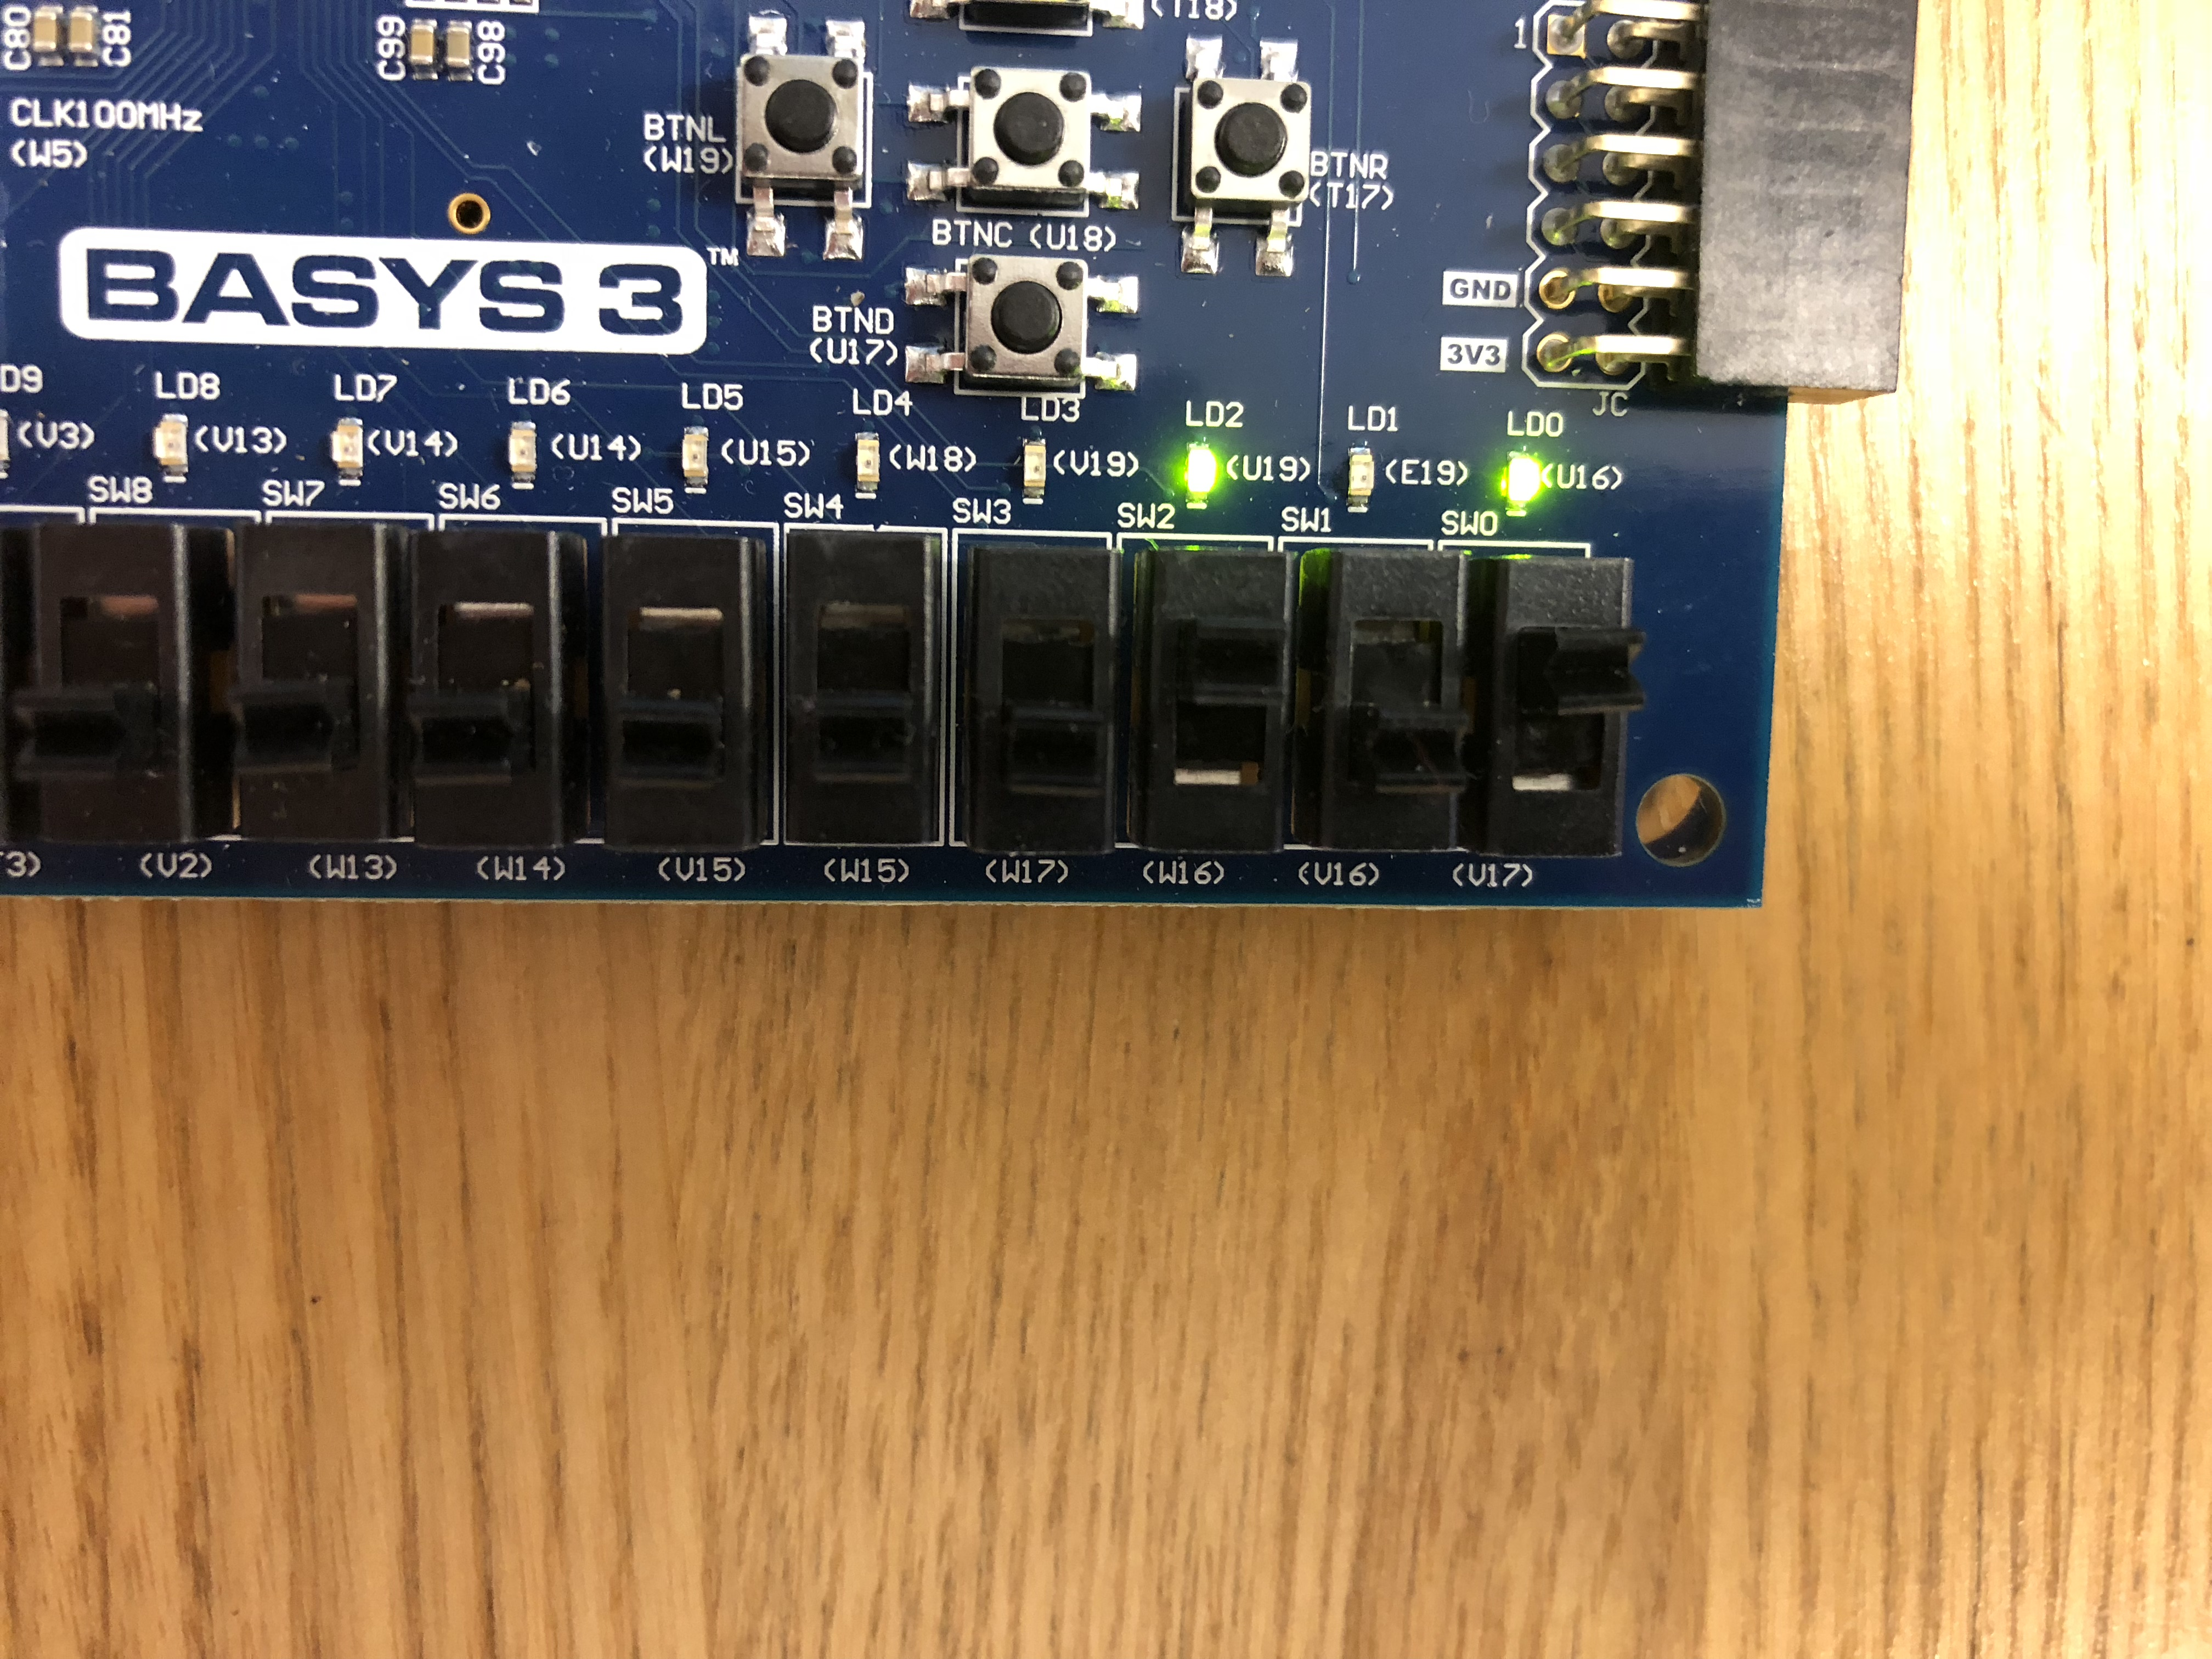
\includegraphics[width=0.5\textwidth]{../report-images/Part1/IMG_3082.jpg}
	\caption{\label{fig:p1img3}The input given by the switches is "0101" and the output shown by the LEDs is "101".}
\end{center}
\end{figure}

\begin{figure}[H]
\begin{center}
	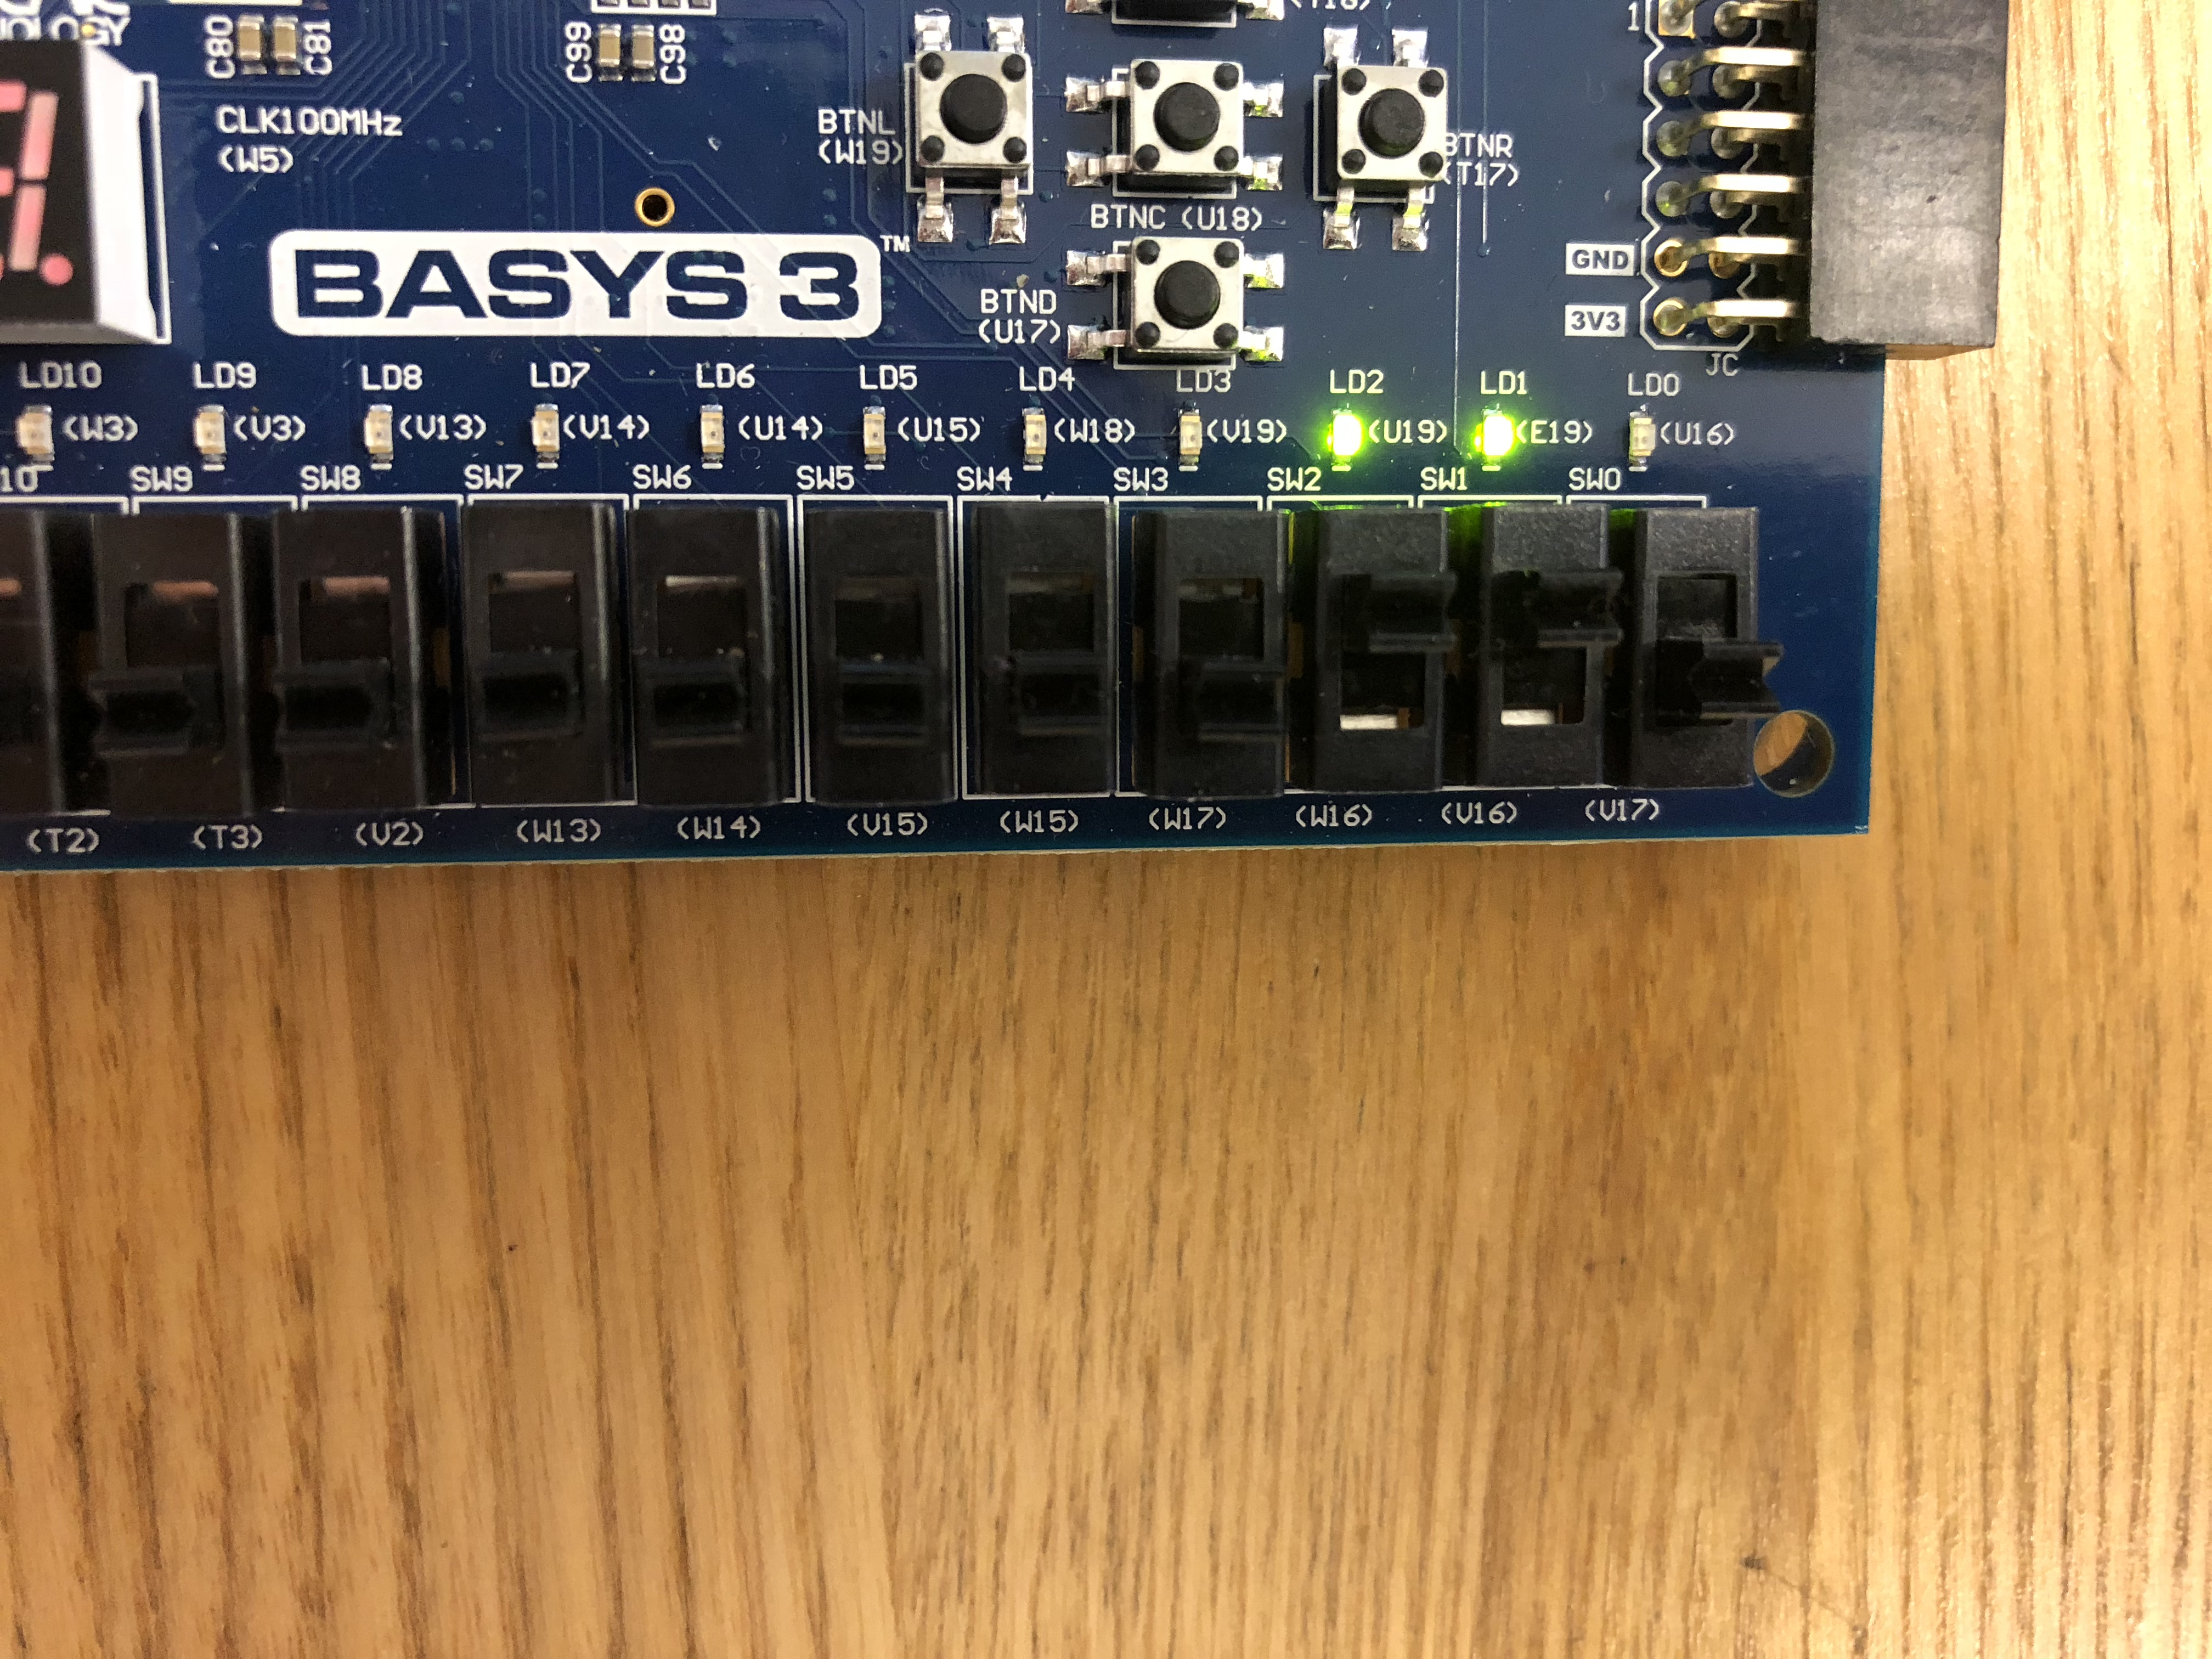
\includegraphics[width=0.5\textwidth]{../report-images/Part1/IMG_3083.jpg}
	\caption{\label{fig:p1img4}The input given by the switches is "0111" and the output shown by the LEDs is "111".}
\end{center}
\end{figure}

\begin{figure}[H]
\begin{center}
	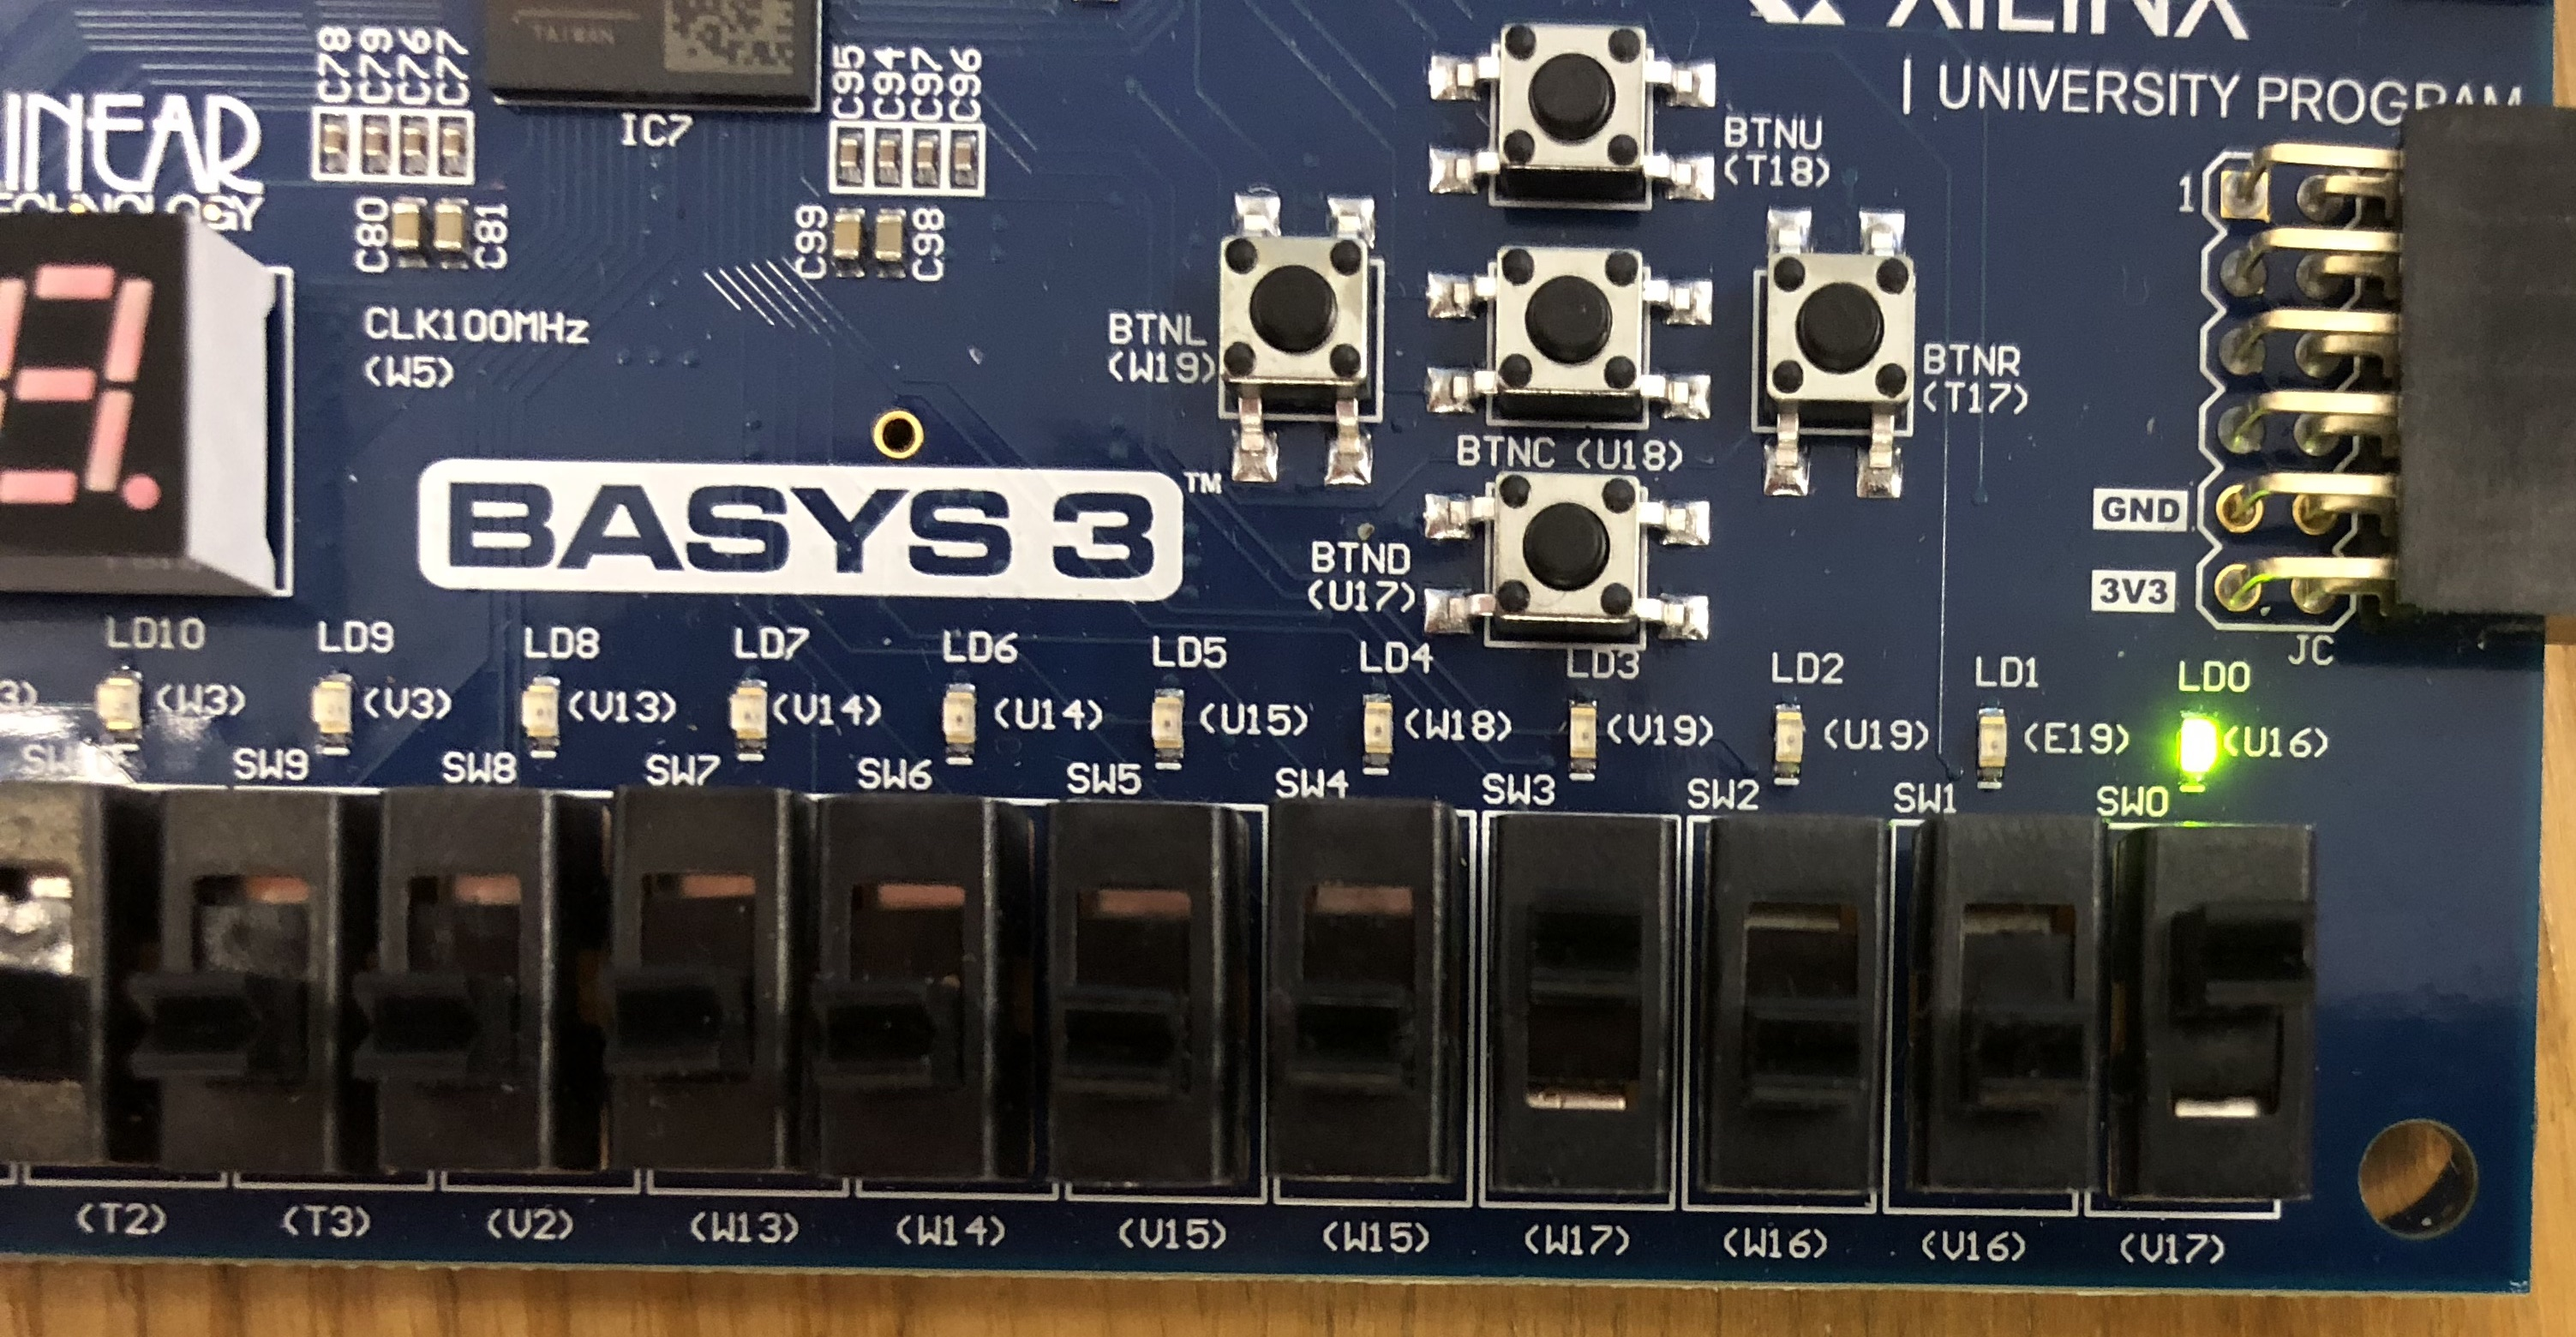
\includegraphics[width=0.5\textwidth]{../report-images/Part1/IMG_3086.jpg}
	\caption{\label{fig:p1img6}The input given by the switches is "1001" and the output shown by the LEDs is "001".}
\end{center}
\end{figure}

\begin{figure}[H]
\begin{center}
	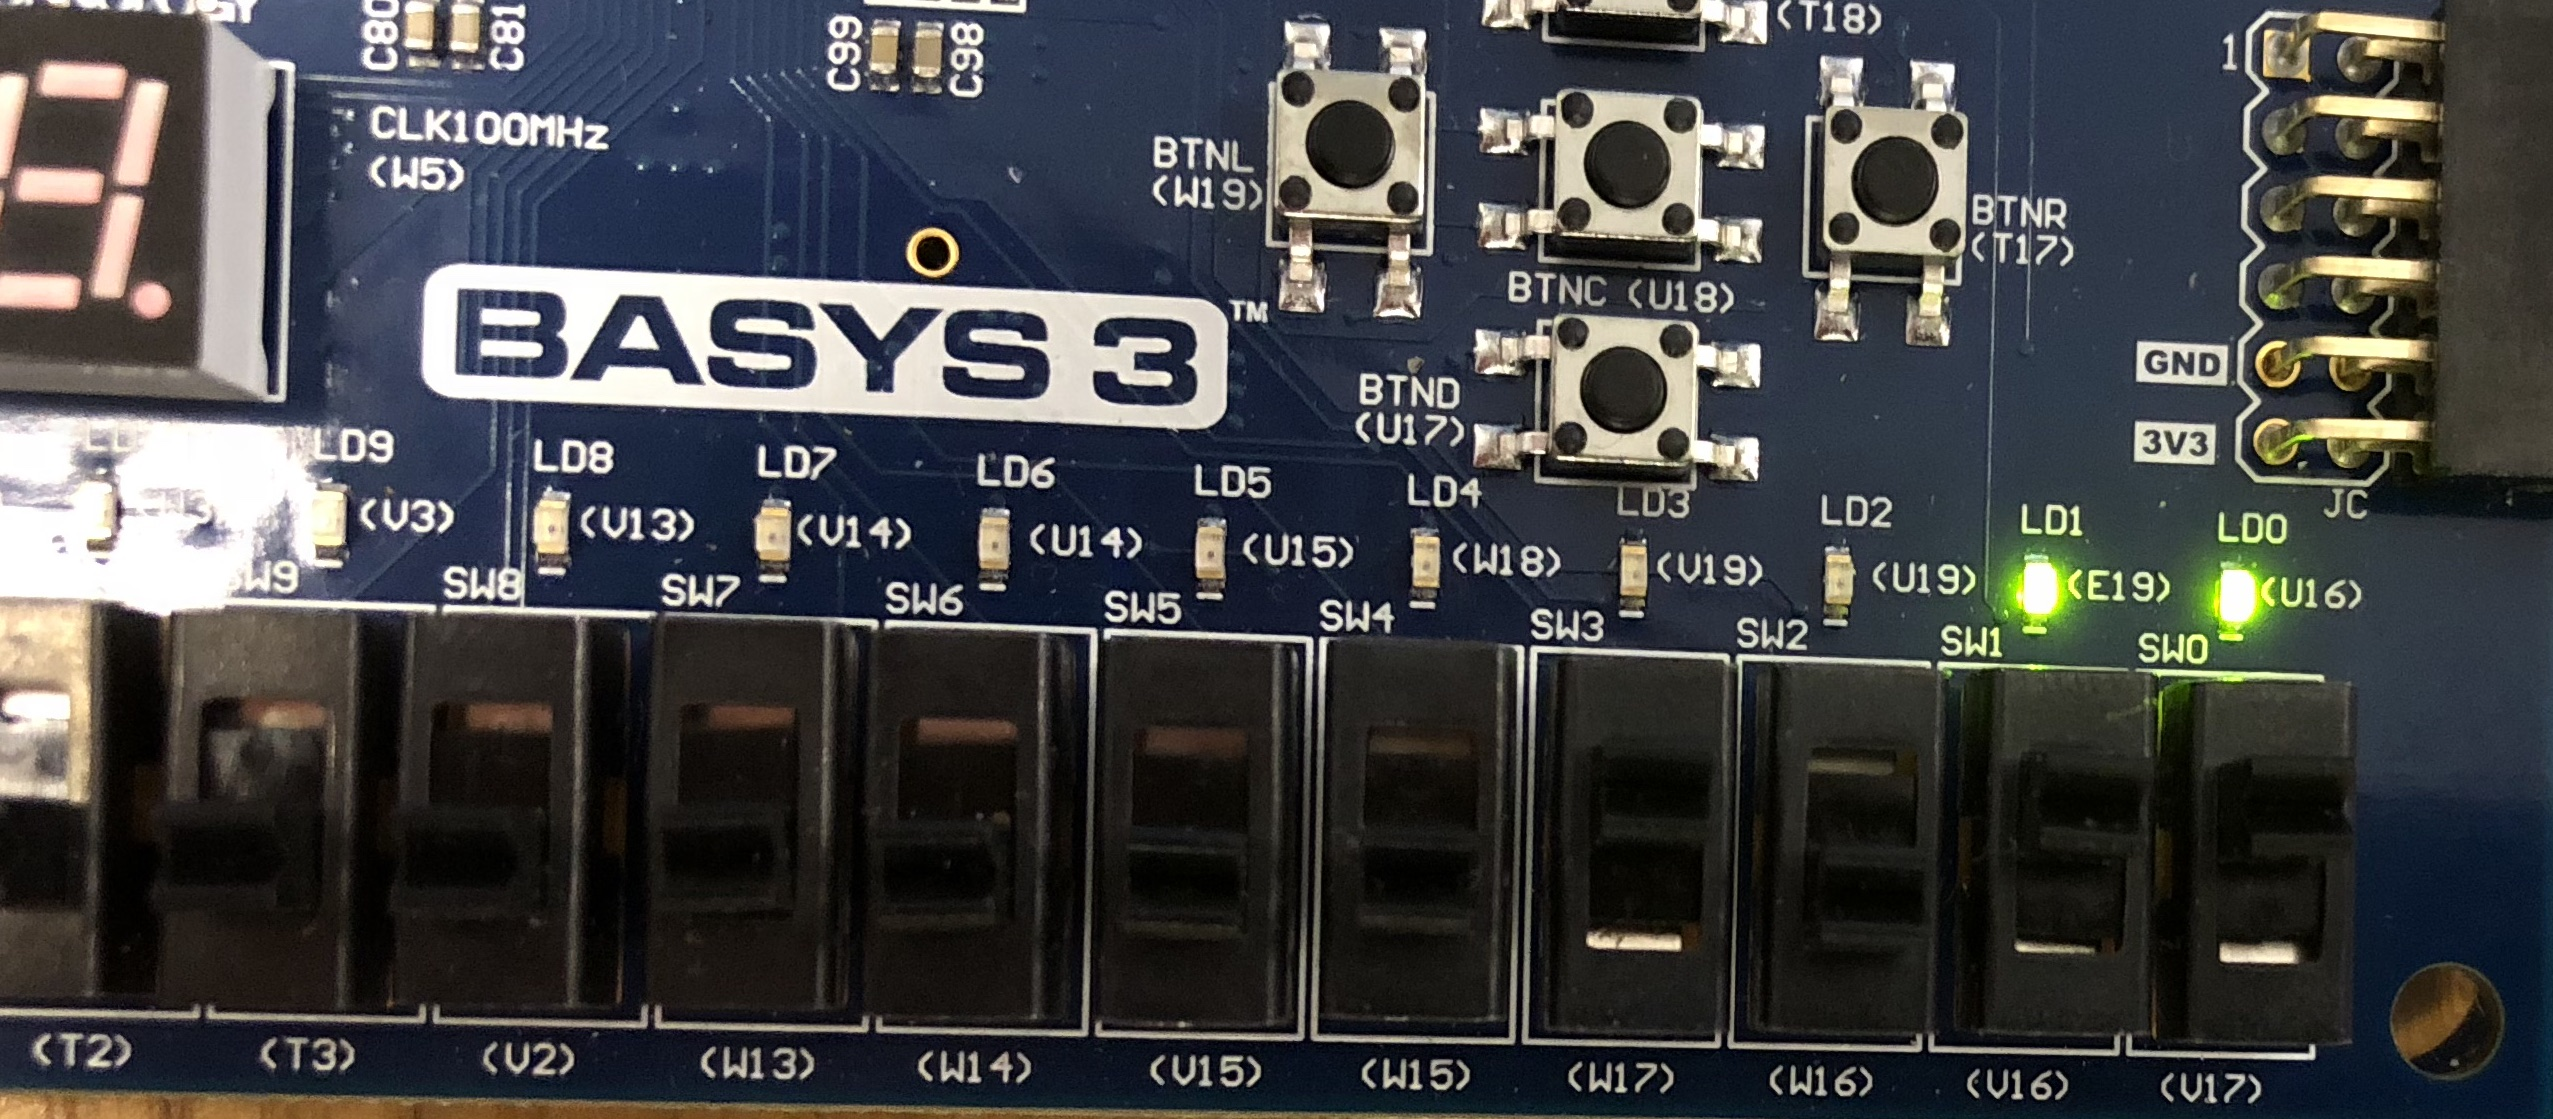
\includegraphics[width=0.5\textwidth]{../report-images/Part1/IMG_3088.jpg}
	\caption{\label{fig:p1img7}The input given by the switches is "1011" and the output shown by the LEDs is "011".}
\end{center}
\end{figure}

\begin{figure}[H]
\begin{center}
	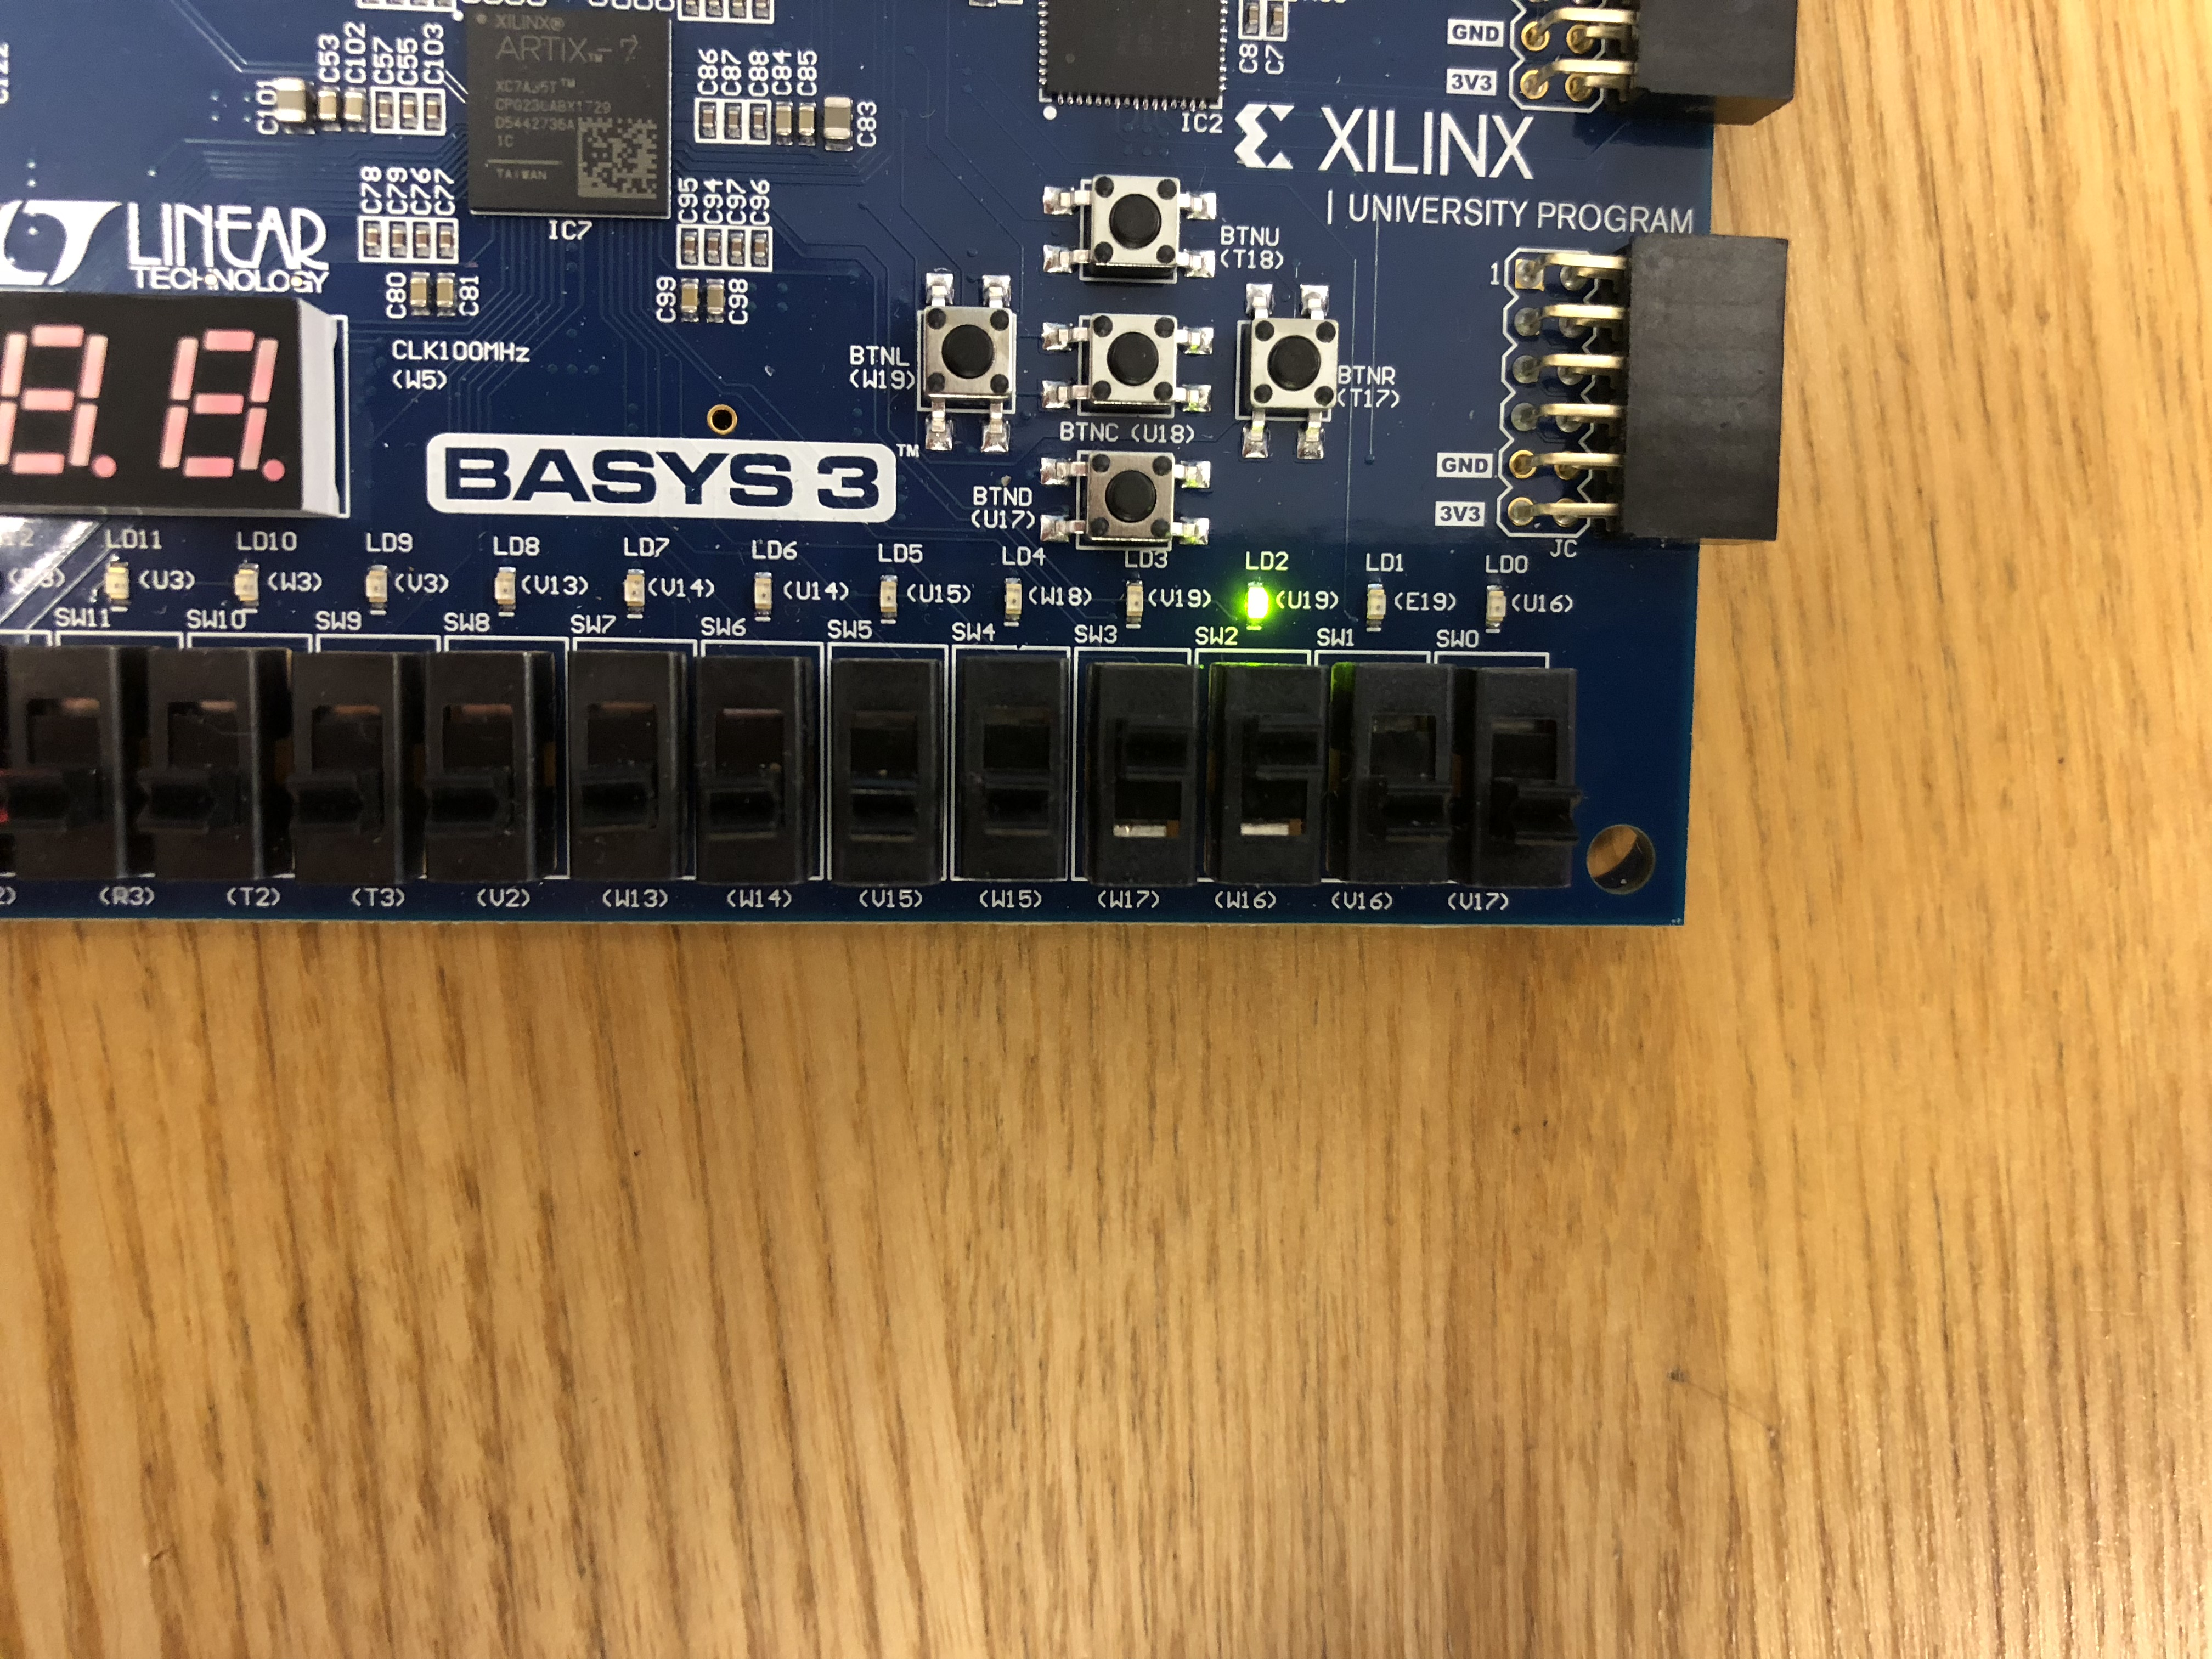
\includegraphics[width=0.5\textwidth]{../report-images/Part1/IMG_3089.jpg}
	\caption{\label{fig:p1img8}The input given by the switches is "1100" and the output shown by the LEDs is "100".}
\end{center}
\end{figure}

\begin{figure}[H]
\begin{center}
	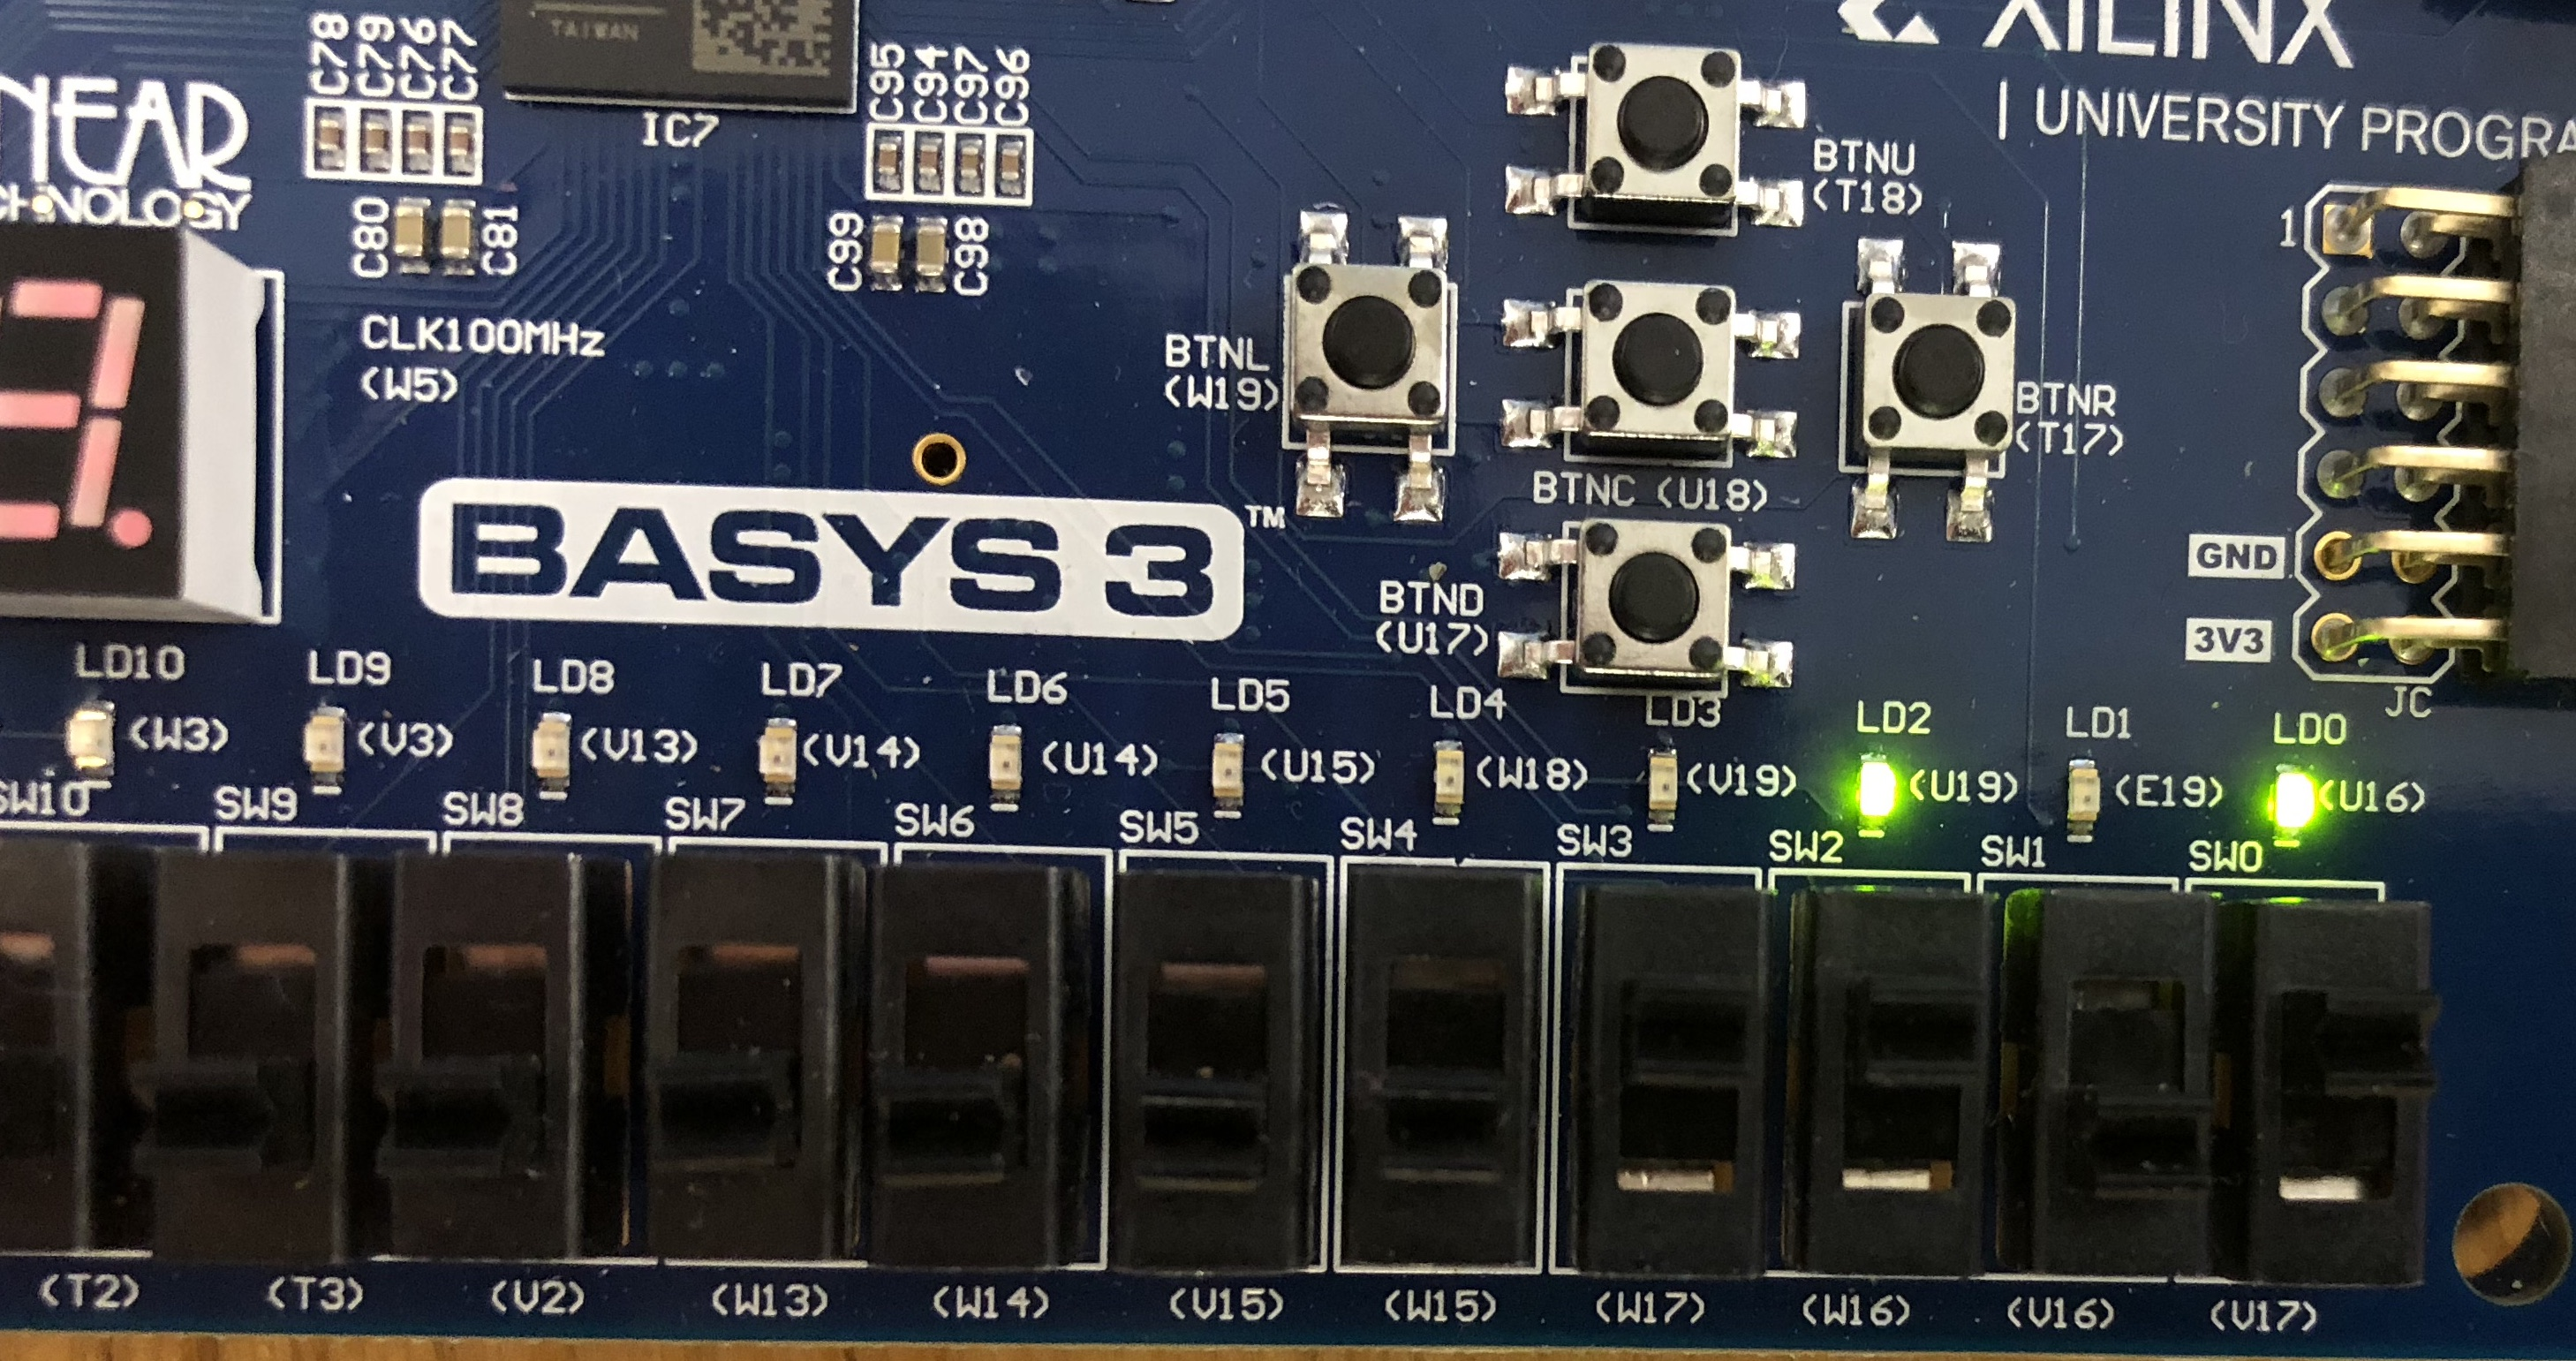
\includegraphics[width=0.5\textwidth]{../report-images/Part1/IMG_3090.jpg}
	\caption{\label{fig:p1img9}The input given by the switches is "1101" and the output shown by the LEDs is "101".}
\end{center}
\end{figure}

\subsection{Problem 2 ROM Multiplexer}

\subsubsection{Background}
This assignment builds completely on the previous assignment by feeding the output of the ROM module into a multiplexer that will output only one of the three bits. This module could be used to work with only specific bits from a given memory word.

\theoremstyle{definition}
\newtheorem{definition}{Definition}
\begin{definition}
Multiplexer: A multiplexer is a module that will pass only specific parts of the given input signal, based on a selector signal from the user.
\end{definition}

\subsubsection{Design Solution}
Our approach was to use the complete entity and architecture from the previous portion of the lab as a component, and feed that information to the multiplexer. Since there are 3 outputs that can be selected, we needed to use a 2-bit input for our multiplexer. However, with 4 possible select inputs and only 3 used, we do have an invalid "sel" input, "11". For this input, we decided to turn on all lights on the 7-segment display, showing an "8". Because 8 is obviously not a value that can be represented by one bit, this shows a clear error state to the user. Valid selections will display the value of the chosen bit, '1' or '0', on the 7-segment display. For reference, a key to 7-segment displays is shown in Figure ~\ref{fig:sevenSeg}. The truth table for this system is shown in Table ~\ref{tab:romMuxTruthTable}. Instead of describing every output to the 7-segment display, Tables ~\ref{tab:romMuxTruthTable1} and ~\ref{tab:romMuxTruthTable2} show the output as 1 or 0. Table ~\ref{tab:sevenSegTruthTable} describes how these outputs are handled with respect to the 7-segments display. Finally, Table ~\ref{tab:romMuxPorts} describes the port assignments for our design.

\begin{figure}[H]
\begin{center}
	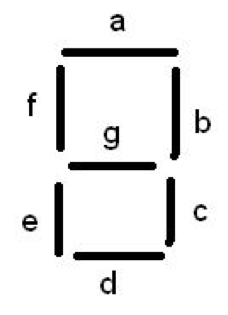
\includegraphics[width=0.2\textwidth]{../../Lab2/report-images/img1.png}
	\caption{\label{fig:sevenSeg}Seven segment display diagram.}
\end{center}
\end{figure}

\begin{minipage}[t]{0.4\textwidth}
\begin{table}[H]
\begin{center}
\begin{tabular}{| l | l | l | l | l | l |}
	\hline
	x & sel & z \\ \hline
	\multirow{3}{*}{0000} & 00 & 0 \\
	& 01 & 0 \\
	& 10 & 0 \\ \hline
	\multirow{3}{*}{0001} & 00 & 1 \\
	& 01 & 0 \\
	& 10 & 0 \\ \hline
	\multirow{3}{*}{0010} & 00 & 0 \\
	& 01 & 1 \\
	& 10 & 0 \\ \hline
	\multirow{3}{*}{0011} & 00 & 1 \\
	& 01 & 1 \\
	& 10 & 0 \\ \hline
	\multirow{3}{*}{0100} & 00 & 0 \\
	& 01 & 0 \\
	& 10 & 1 \\ \hline
	\multirow{3}{*}{0101} & 00 & 1 \\
	& 01 & 0 \\
	& 10 & 1 \\ \hline
	\multirow{3}{*}{0110} & 00 & 0 \\
	& 01 & 1 \\
	& 10 & 1 \\ \hline
	\multirow{3}{*}{0111} & 00 & 1 \\
	& 01 & 1 \\
	& 10 & 1 \\ \hline

\end{tabular}
\caption{\label{tab:romMuxTruthTable1}Truth Table for addresses 0000 through 0111.}
\end{center}
\end{table}
\end{minipage}
\begin{minipage}[t]{0.2\textwidth}
\end{minipage}
\begin{minipage}[t]{0.4\textwidth}
\begin{table}[H]
\begin{center}
\begin{tabular}{| l | l | l | l | l | l |}
	\hline
	x & sel & z \\ \hline
	\multirow{3}{*}{1000} & 00 & 0 \\
	& 01 & 0 \\
	& 10 & 0 \\ \hline
	\multirow{3}{*}{1001} & 00 & 1 \\
	& 01 & 0 \\
	& 10 & 0 \\ \hline
	\multirow{3}{*}{1010} & 00 & 0 \\
	& 01 & 1 \\
	& 10 & 0 \\ \hline
	\multirow{3}{*}{1011} & 00 & 1 \\
	& 01 & 1 \\
	& 10 & 0 \\ \hline
	\multirow{3}{*}{1100} & 00 & 0 \\
	& 01 & 0 \\
	& 10 & 1 \\ \hline
	\multirow{3}{*}{1101} & 00 & 1 \\
	& 01 & 0 \\
	& 10 & 1 \\ \hline
	\multirow{3}{*}{1110} & 00 & 0 \\
	& 01 & 1 \\
	& 10 & 1 \\ \hline
	\multirow{3}{*}{1111} & 00 & 1 \\
	& 01 & 1 \\
	& 10 & 1 \\ \hline
\end{tabular}
\caption{\label{tab:romMuxTruthTable2}Truth table for addresses 1000 through 1111.}
\end{center}
\end{table}
\end{minipage}

\begin{table}[H]
\begin{center}
\begin{tabular}{| l | l | l | l | l | l | l | l |}
	\hline
	Output Bit & z0 & z1 & z2 & z3 & z4 & z5 & z6 \\ \hline
	0 & 0 & 0 & 0 & 0 & 0 & 0 & 1 \\ \hline
	1 & 1 & 0 & 0 & 1 & 1 & 1 & 1 \\ \hline 
\end{tabular}
\caption{\label{tab:sevenSegTruthTable}Truth table for seven segment displayed based on the output.}
\end{center}
\end{table}

\begin{table}{H}
\begin{center}
\begin{tabular}{| l | l | l |}
	\hline
	Bit & Label & Port \\ \hline
	x3 & Switch 3 & W17 \\ \hline
	x2 & Switch 2 & W16 \\ \hline
	x1 & Switch 1 & V16 \\ \hline
	x0 & Switch 0 & V17 \\ \hline
	z0 & CA & W7 \\ \hline
	z1 & CB & W6 \\ \hline
	z2 & CC & U8 \\ \hline
	z3 & CD & V8 \\ \hline
	z4 & CE & U5 \\ \hline
	z5 & CF & V5 \\ \hline
	z6 & CG & U7 \\ \hline
\end{tabular}
\caption{\label{tab:romMuxPorts}Port assignments for ROM and multiplexer design.}
\end{center}
\end{table}

\subsubsection{Results}
For our ROM and multiplexer circuit to operate as intended, we did have to rotate the output bits for '1' to the right by 1. A misread of the 7-segment diagram led to an initial output of "0011111" for the seven segment display, which was incorrect. However, once that adjustment was made our circuit functioned exactly as expected. A set of the results are displayed in figures ~\ref{fig:p1img1} through ~\ref{fig:p2img13}.

\begin{figure}[H]
\begin{center}
	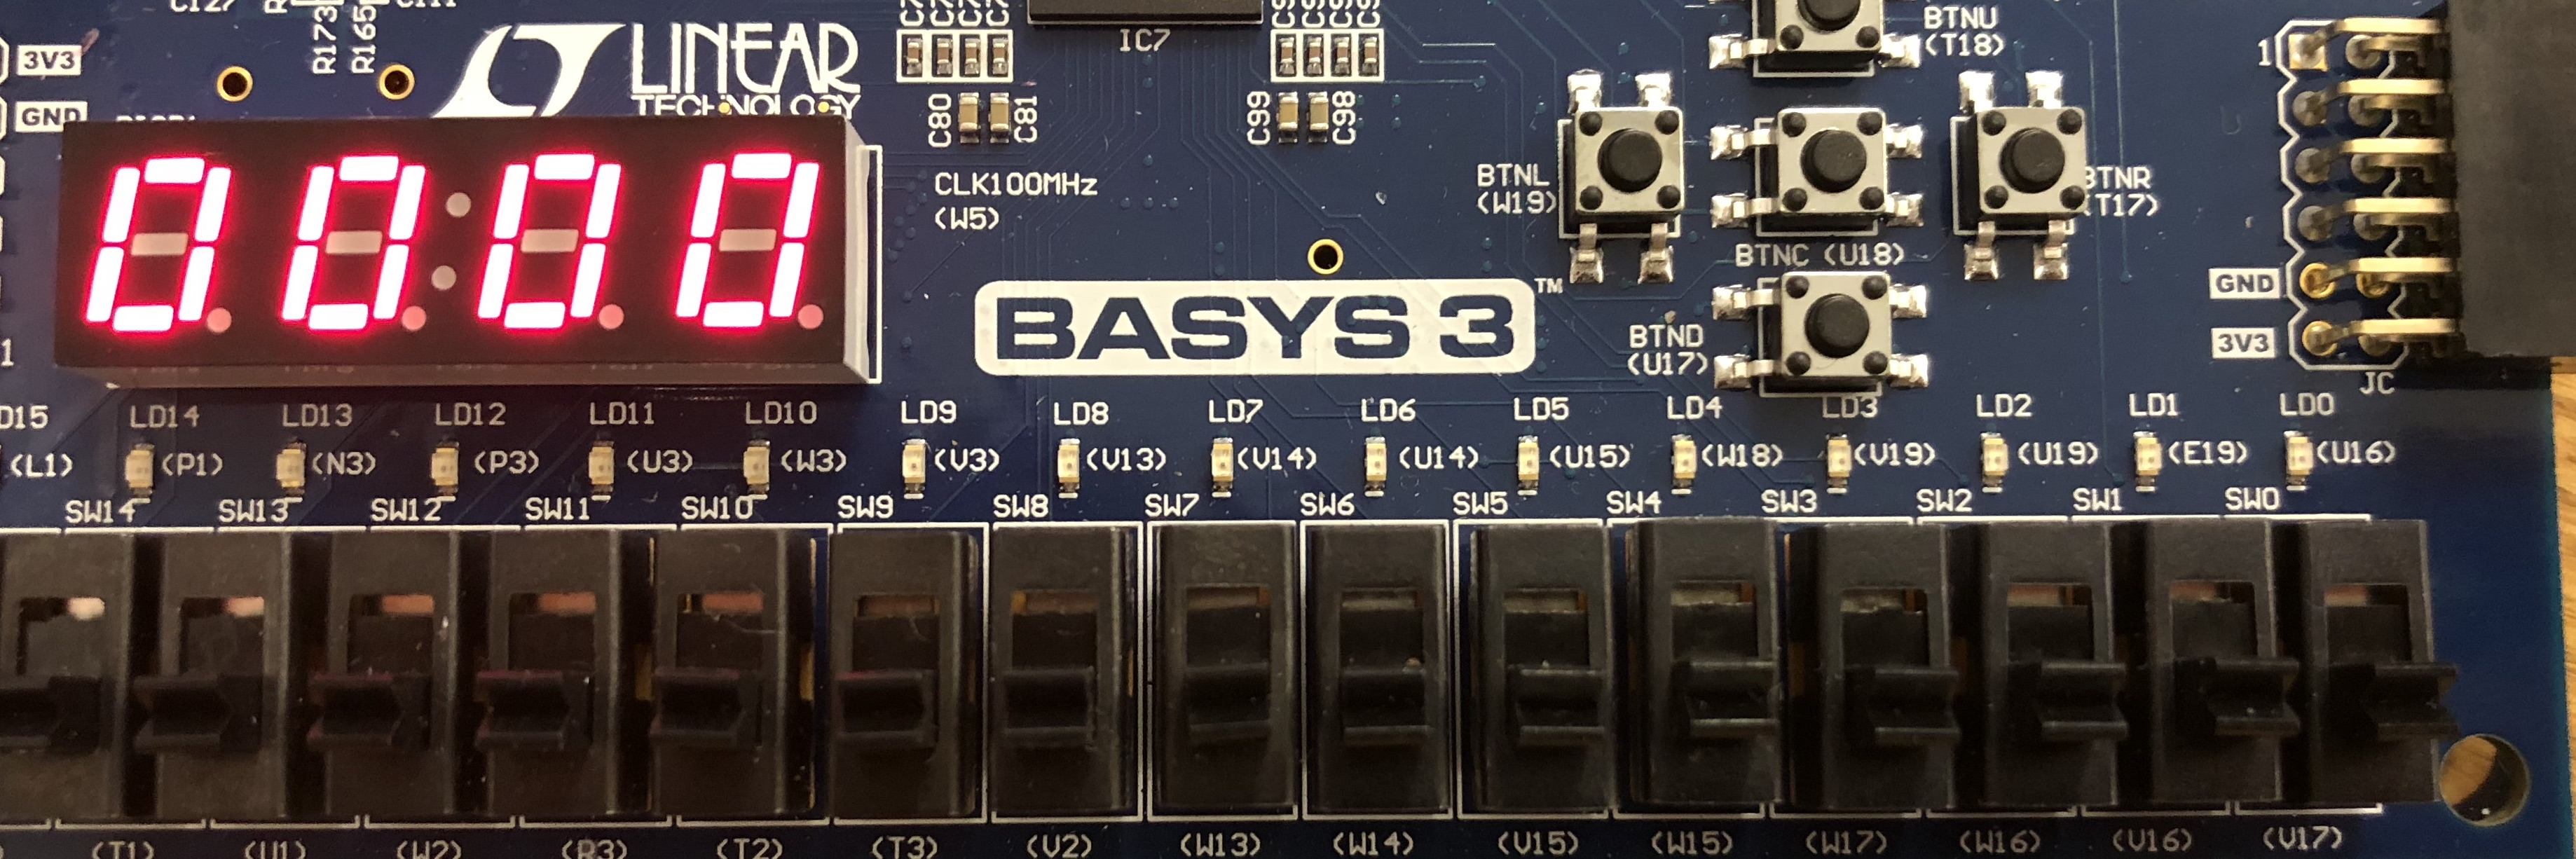
\includegraphics[width=0.5\textwidth]{../report-images/Part2/IMG_3095.jpg}
	\caption{\label{fig:p2img1}The input given by the switches is "0000", select is "00", therefore the output shown by the 7-segment display is "0".}
\end{center}
\end{figure}

\begin{figure}[H]
\begin{center}
	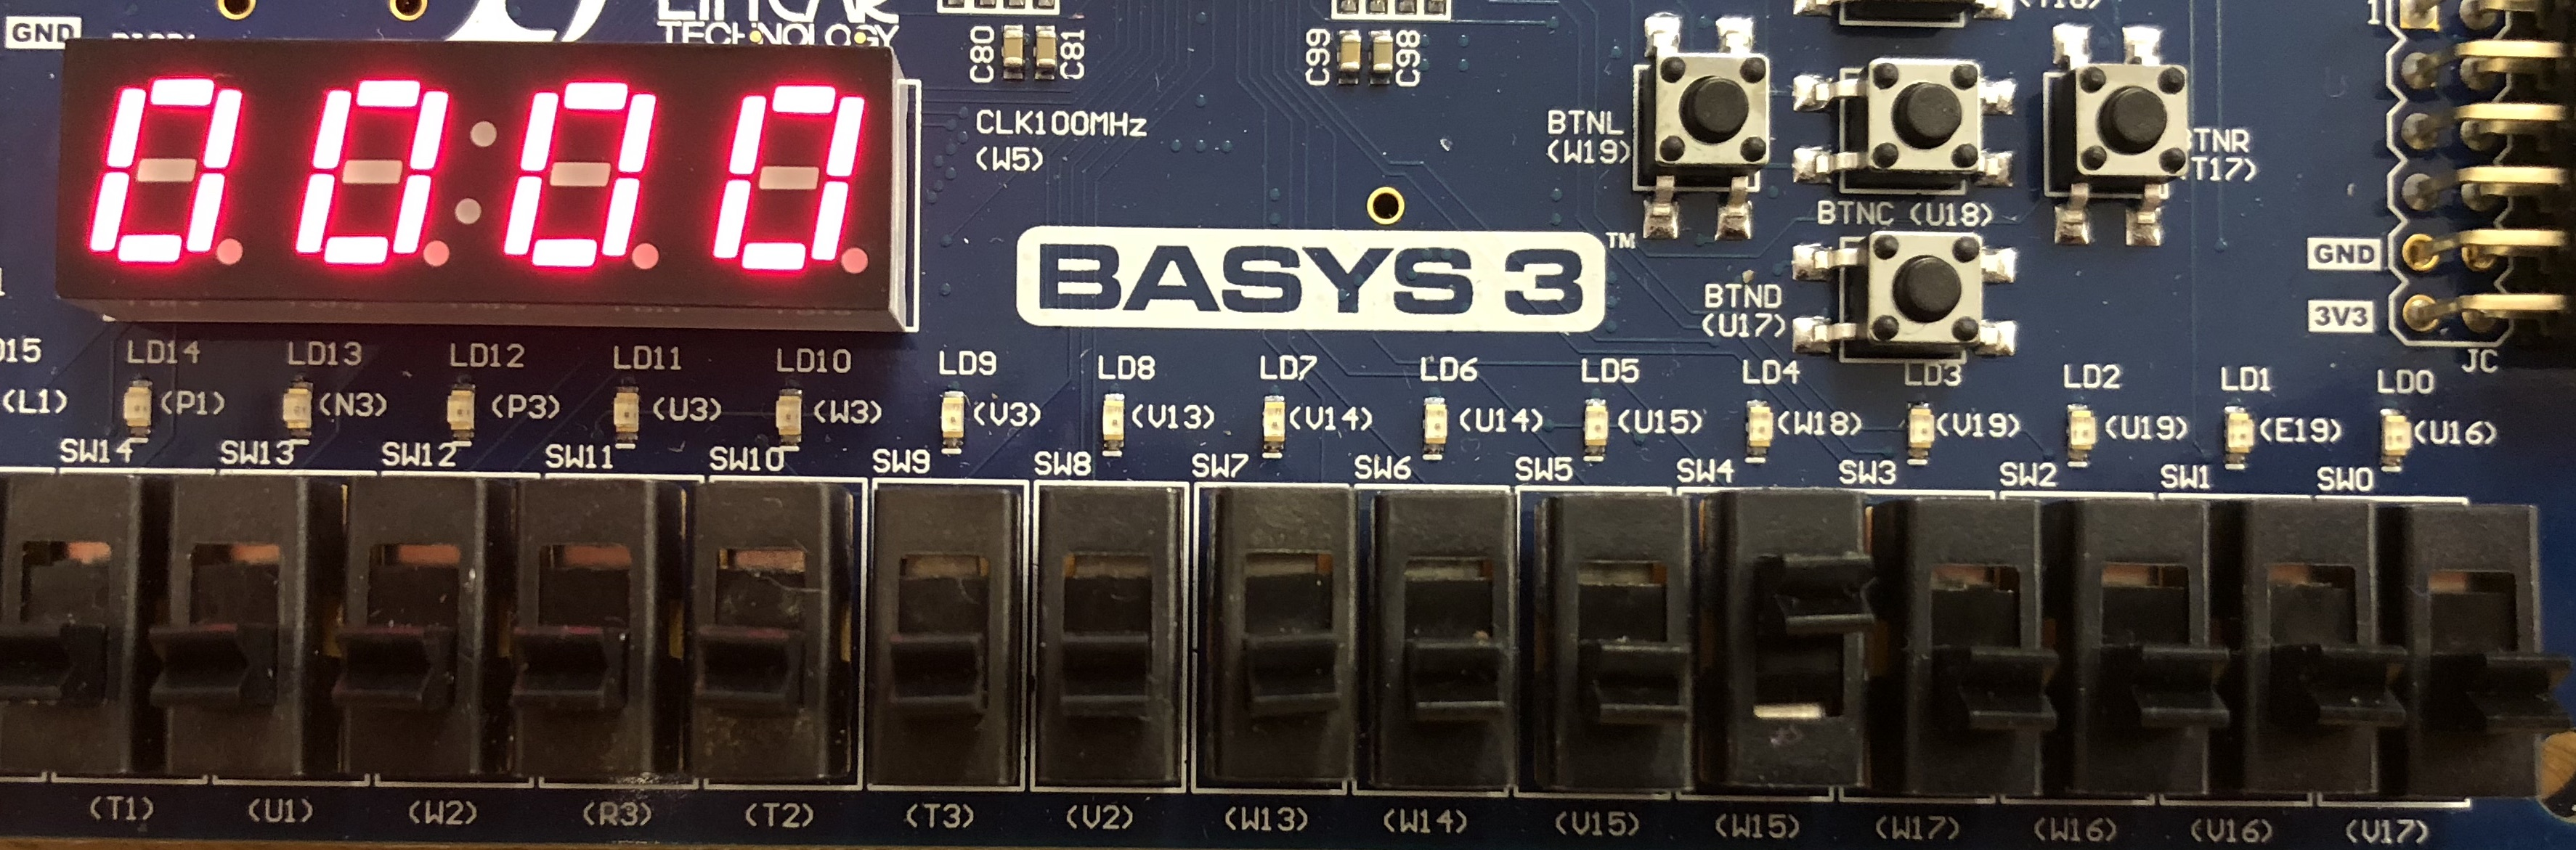
\includegraphics[width=0.5\textwidth]{../report-images/Part2/IMG_3096.jpg}
	\caption{\label{fig:p2img2}The input given by the switches is "0000", select is "01", therefore the output shown by the 7-segment display is "0".}
\end{center}
\end{figure}

\begin{figure}[H]
\begin{center}
	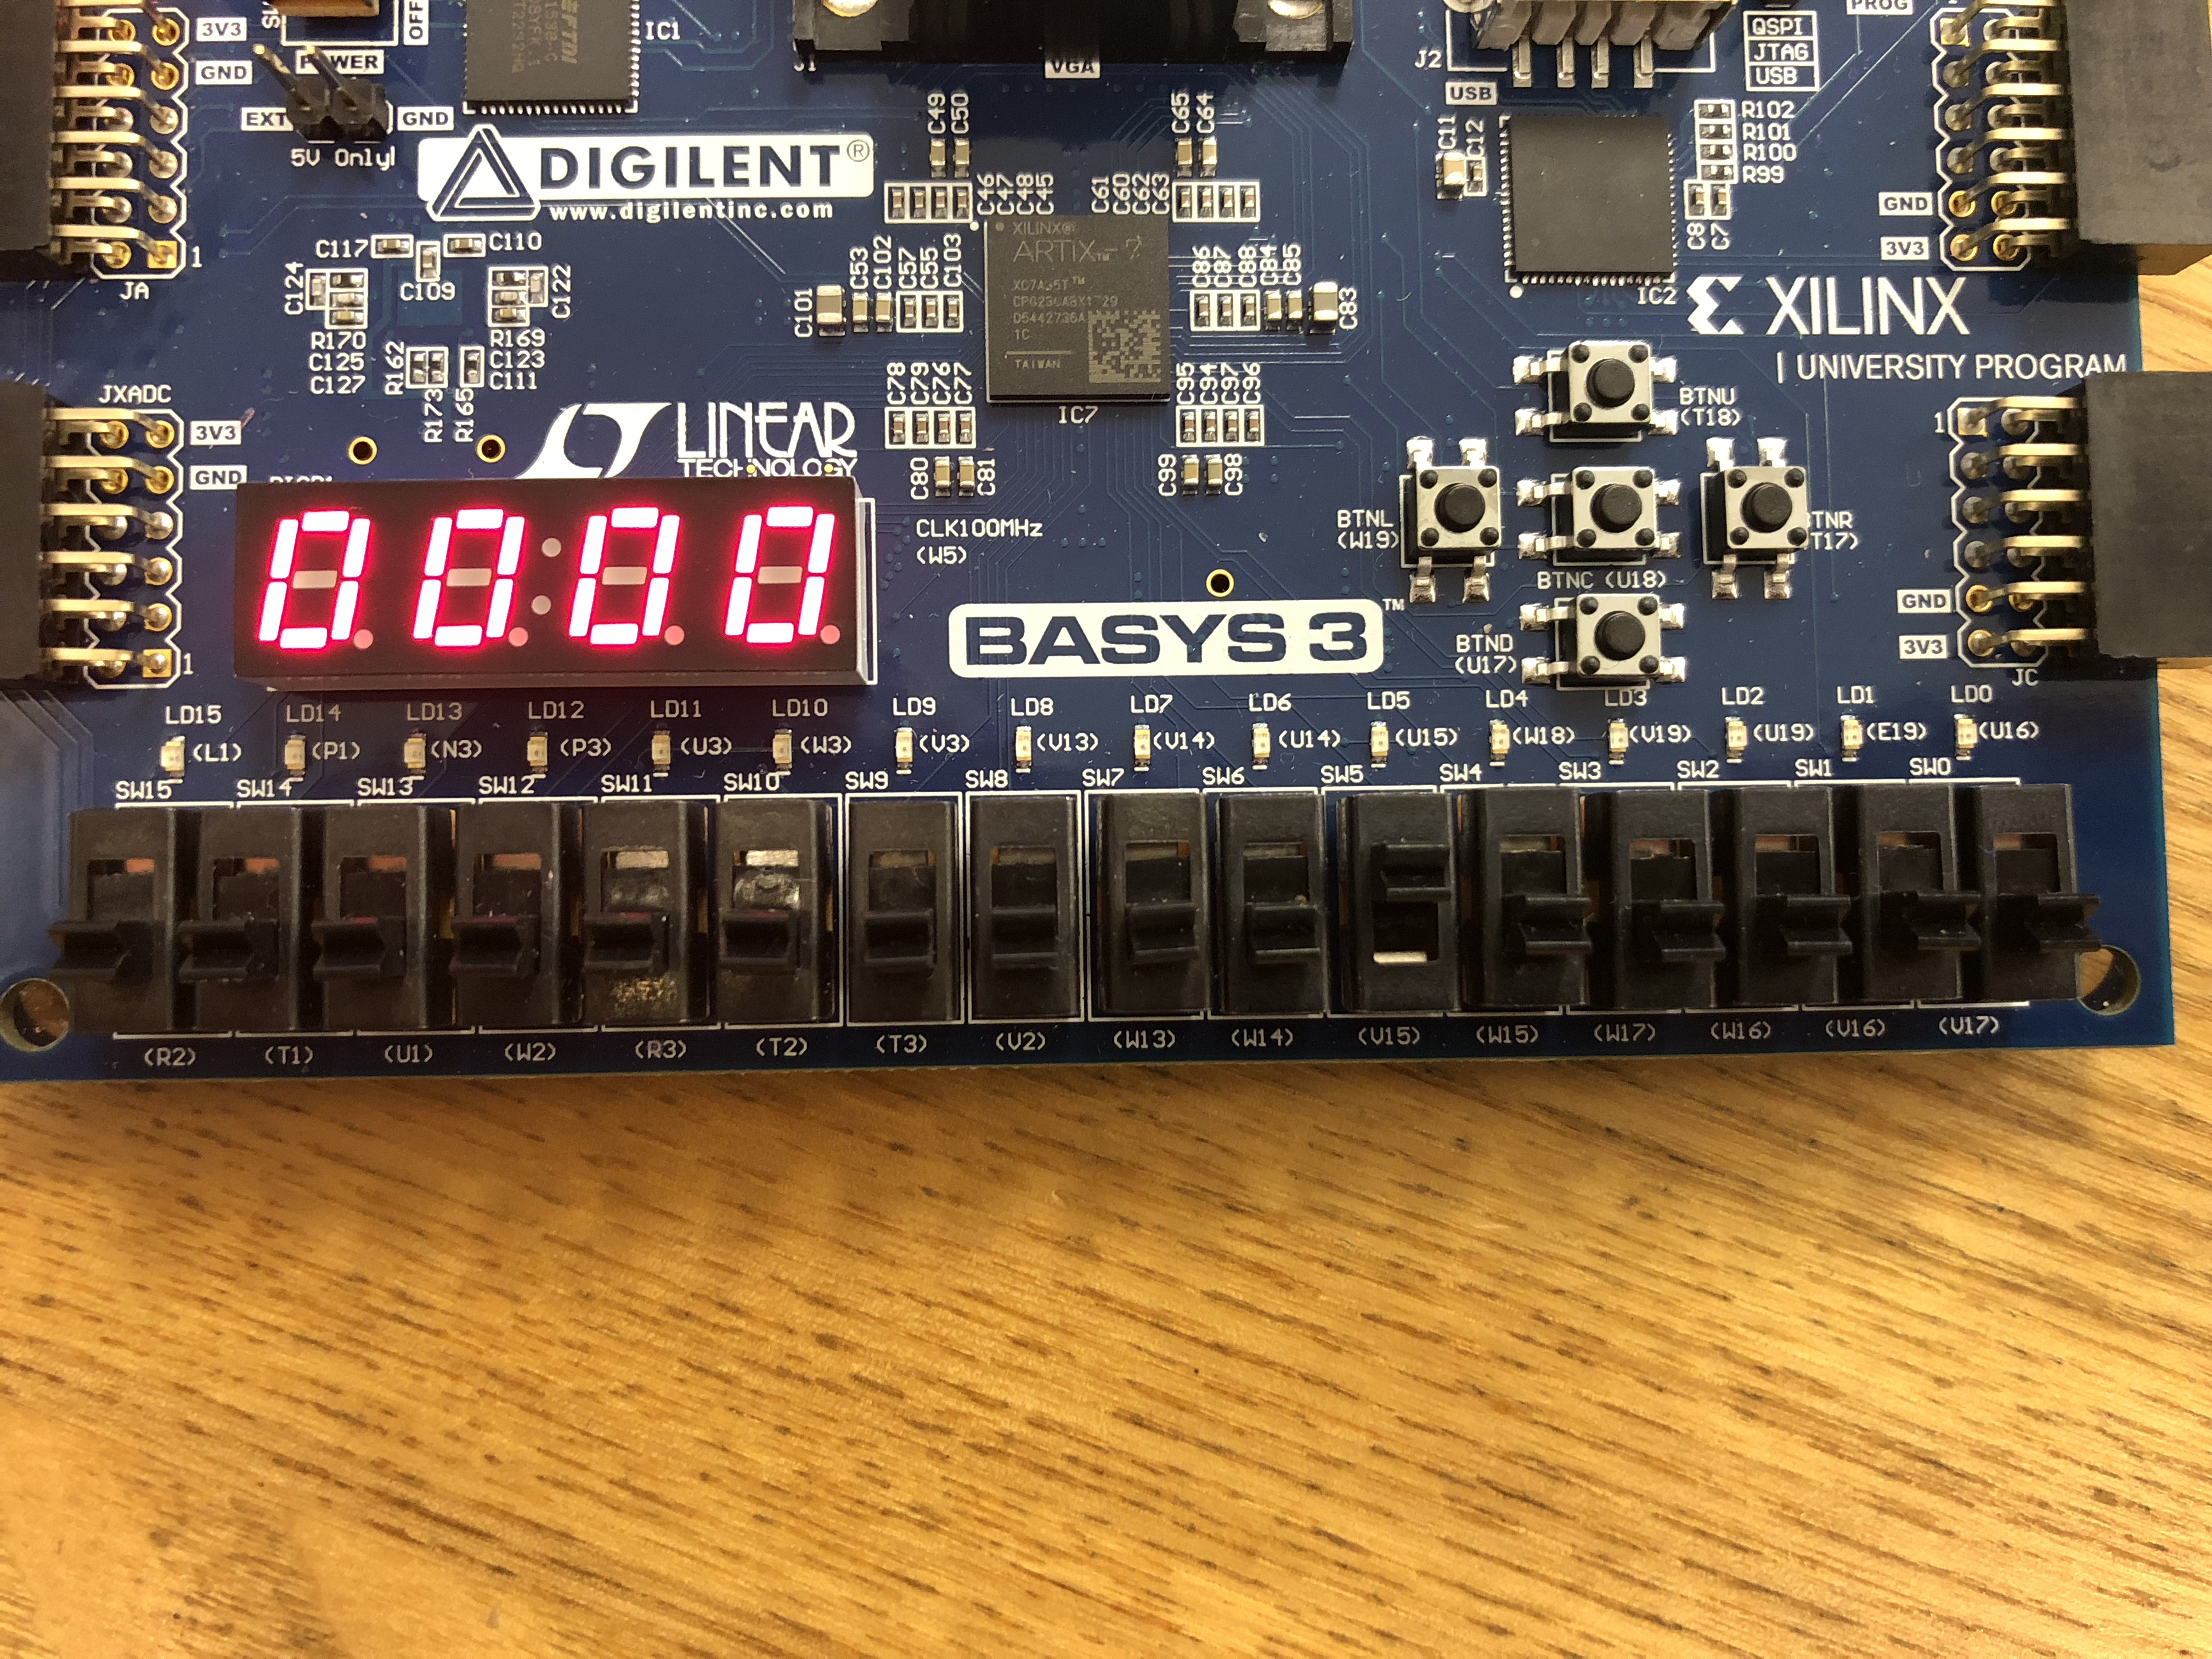
\includegraphics[width=0.5\textwidth]{../report-images/Part2/IMG_3097.jpg}
	\caption{\label{fig:p2img3}The input given by the switches is "0000", select is "10", therefore the output shown by the 7-segment display is "0".}
\end{center}
\end{figure}

\begin{figure}[H]
\begin{center}
	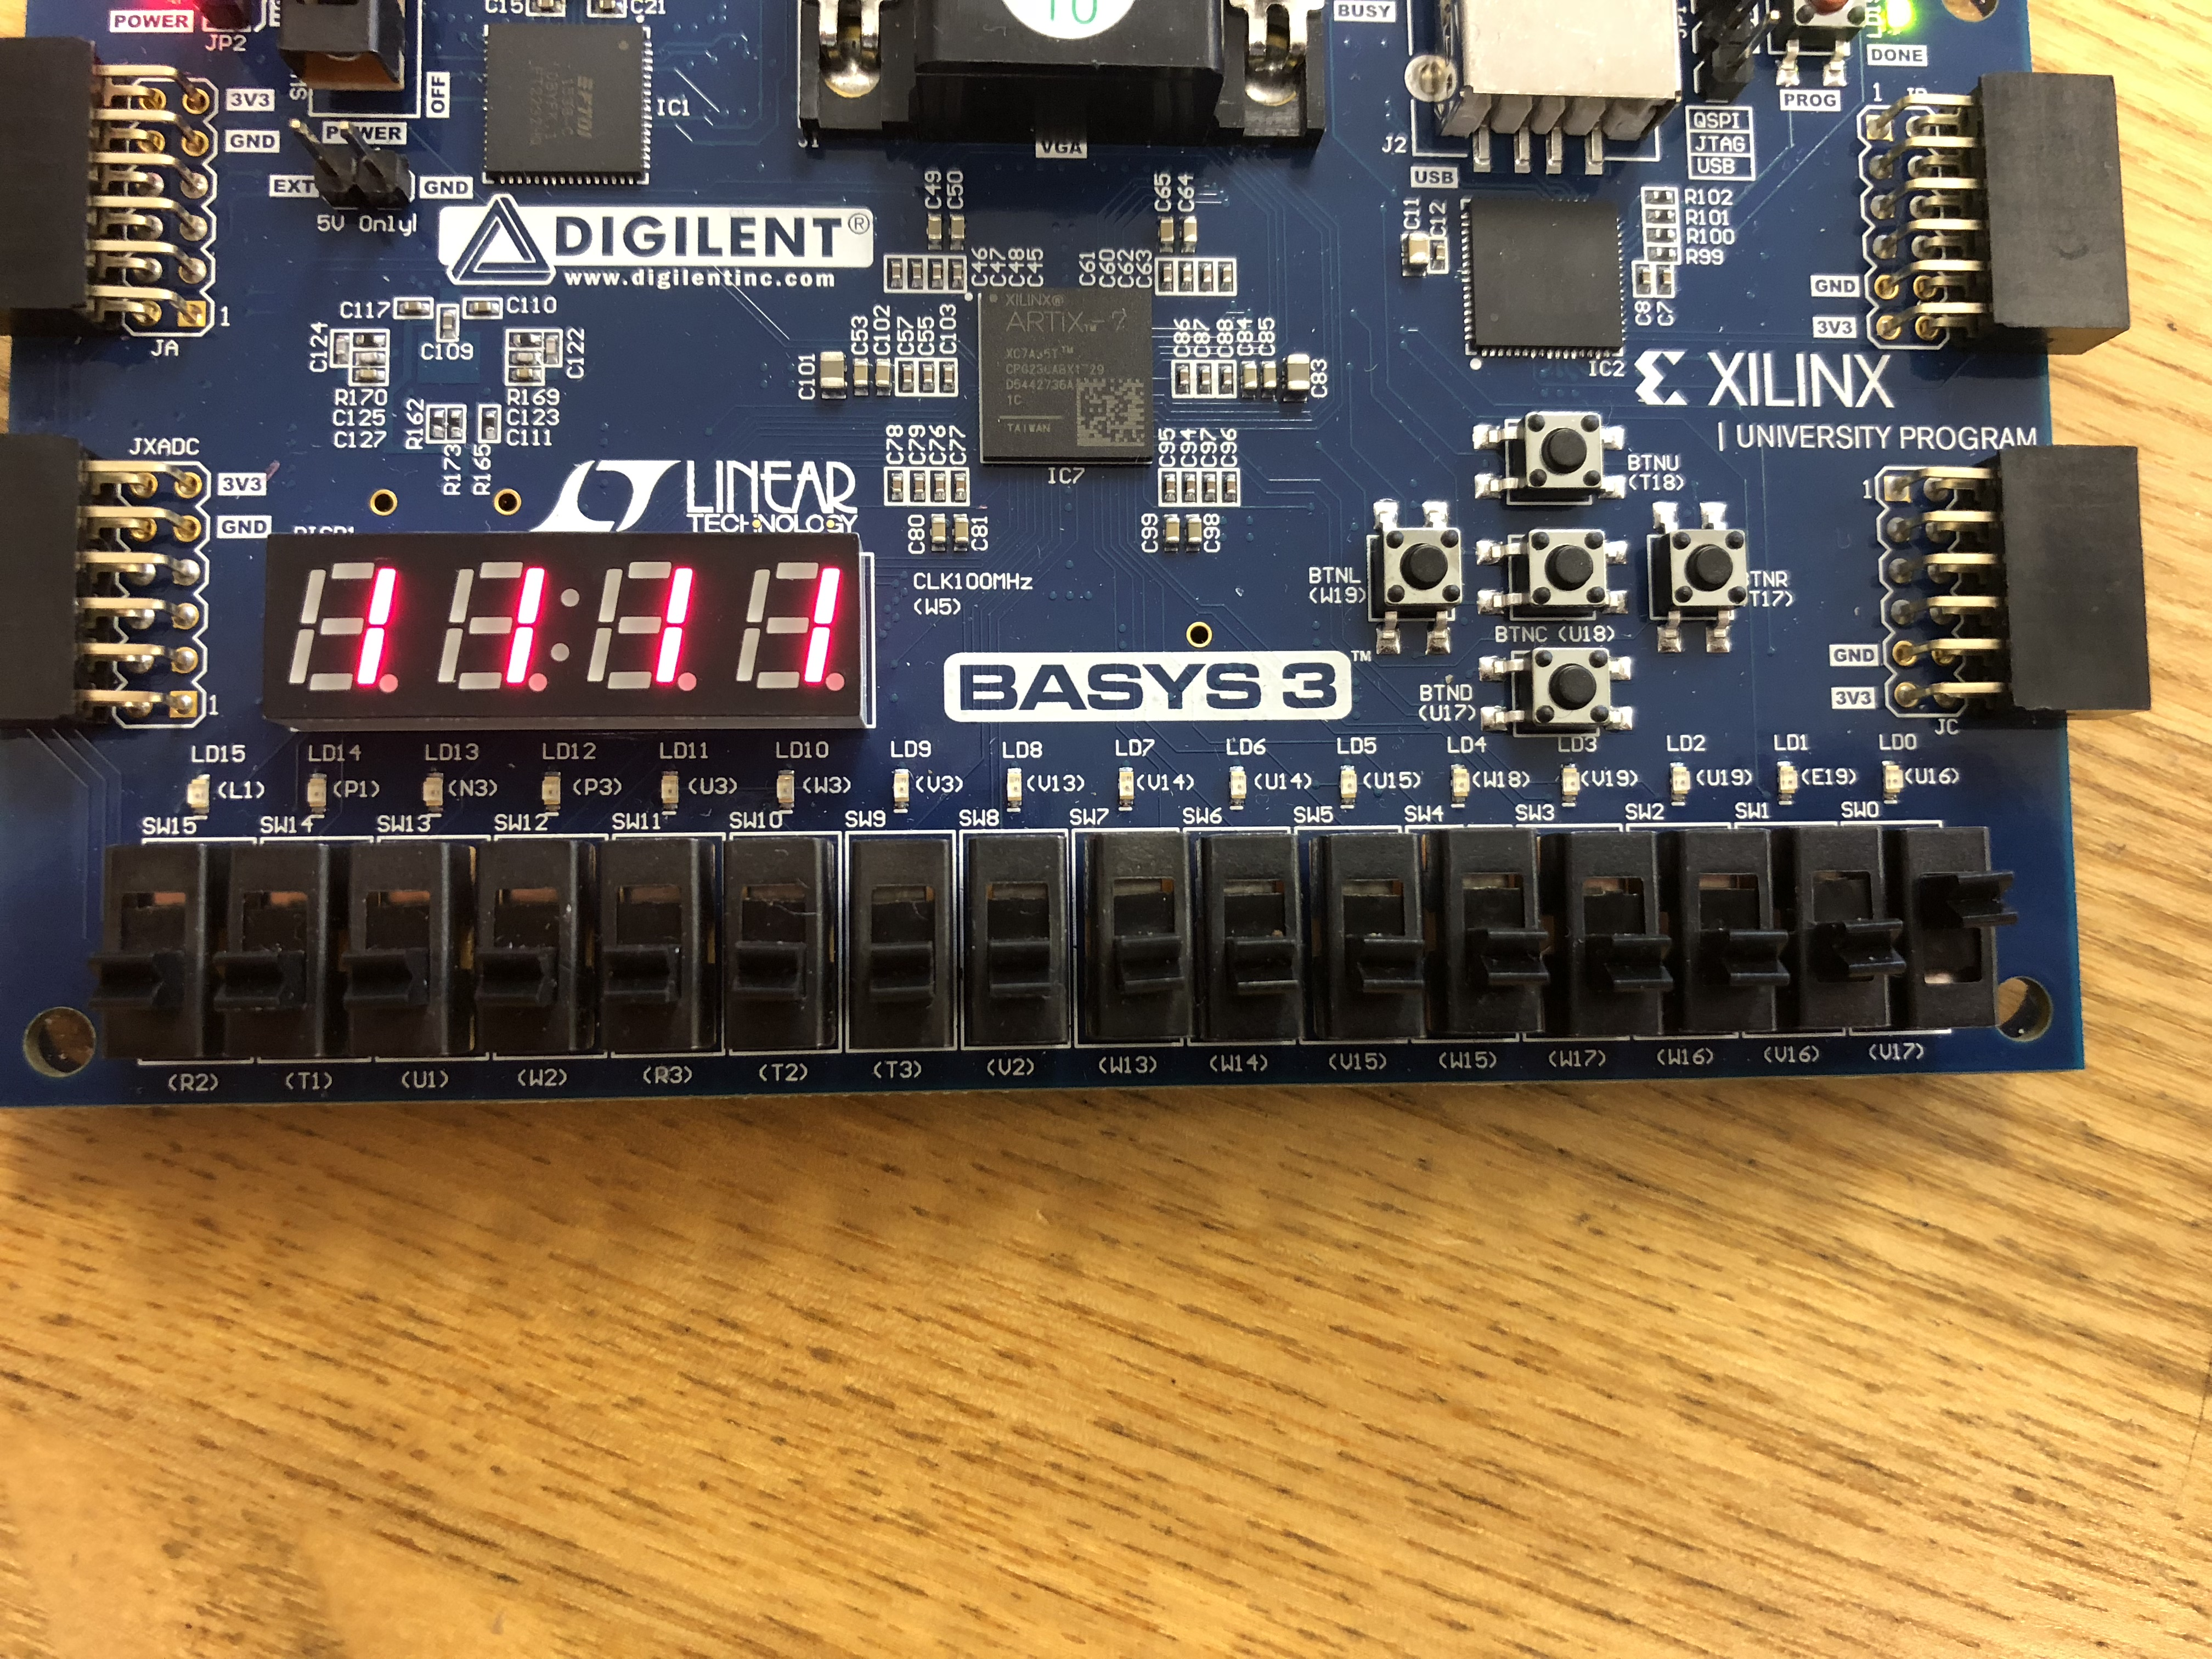
\includegraphics[width=0.5\textwidth]{../report-images/Part2/IMG_3098.jpg}
	\caption{\label{fig:p2img4}The input given by the switches is "0001", select is "00", therefore the output shown by the 7-segment display is "1".}
\end{center}
\end{figure}

\begin{figure}[H]
\begin{center}
	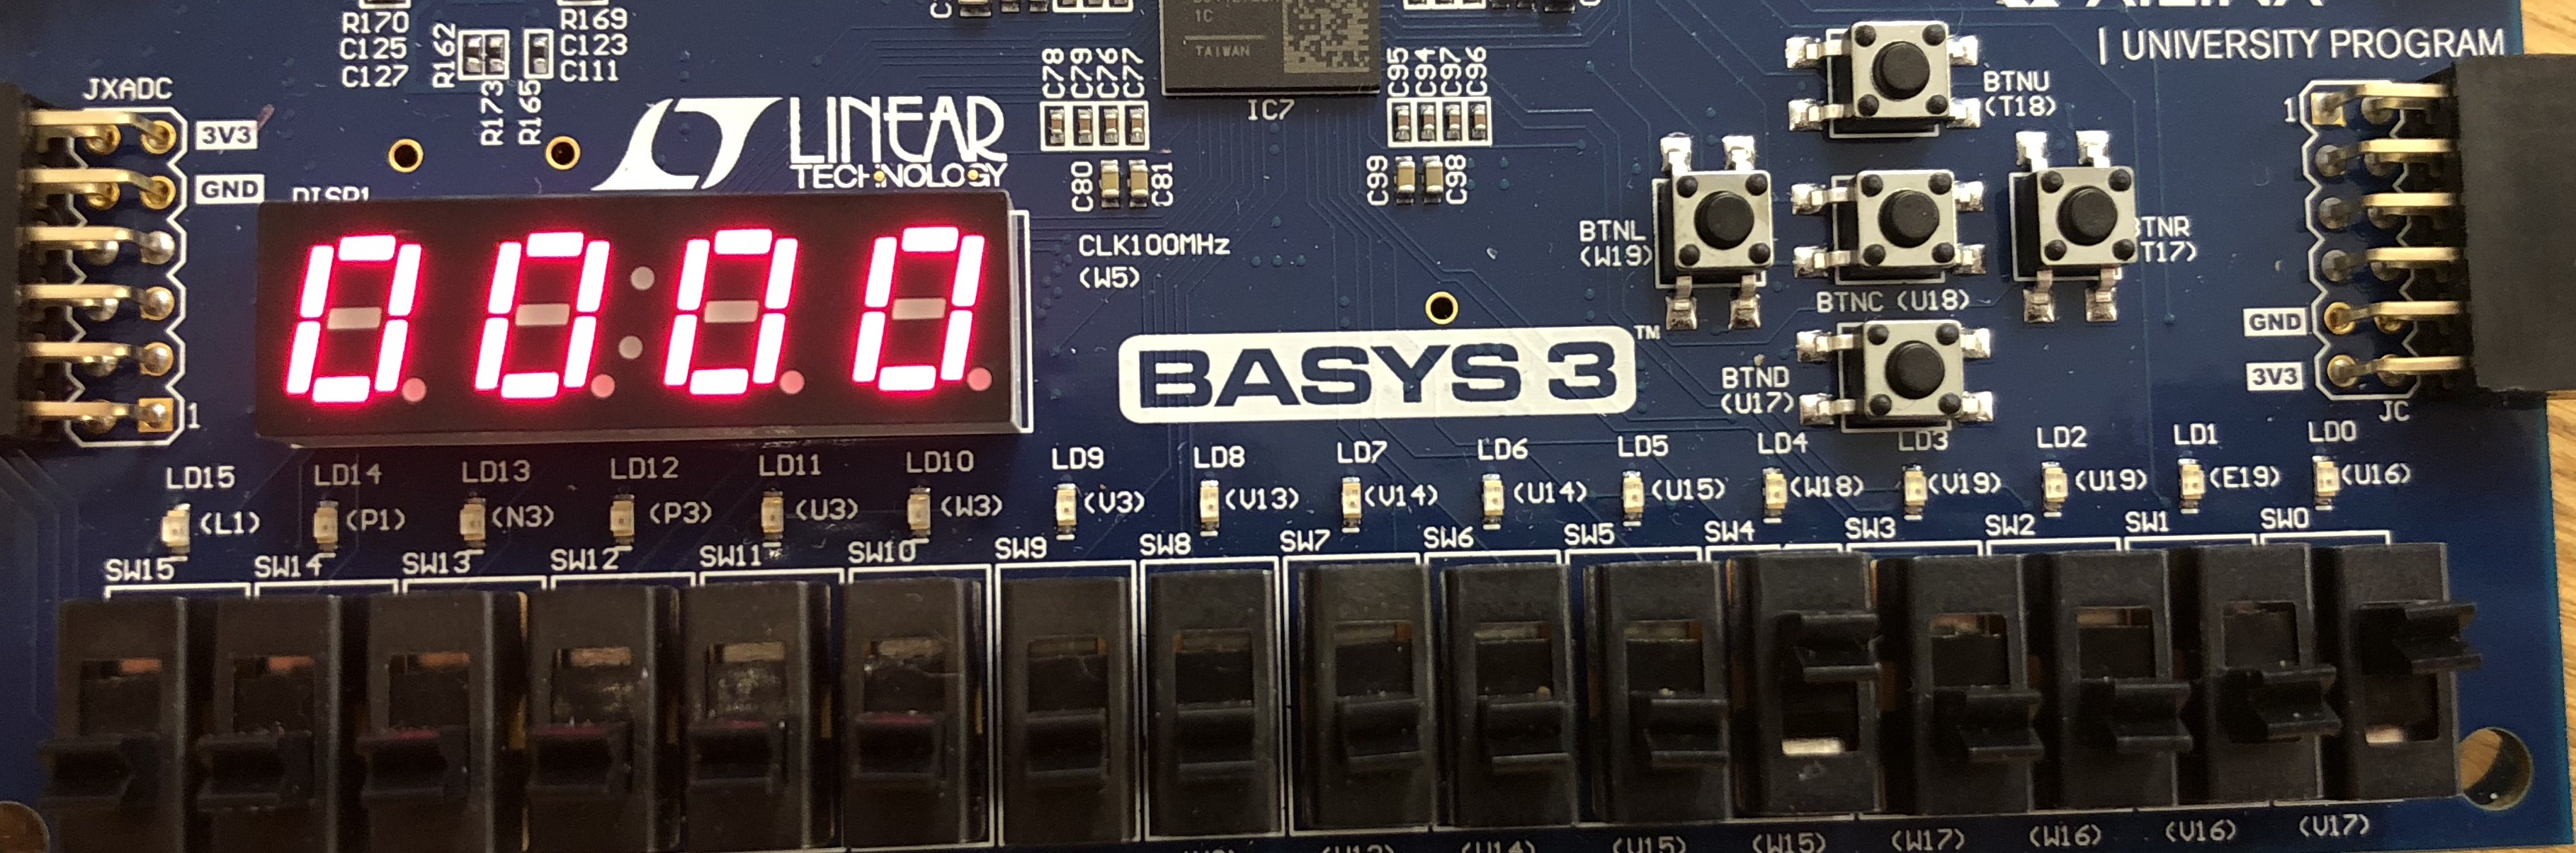
\includegraphics[width=0.5\textwidth]{../report-images/Part2/IMG_3099.jpg}
	\caption{\label{fig:p2img5}The input given by the switches is "0001", select is "01", therefore the output shown by the 7-segment display is "0".}
\end{center}
\end{figure}

\begin{figure}[H]
\begin{center}
	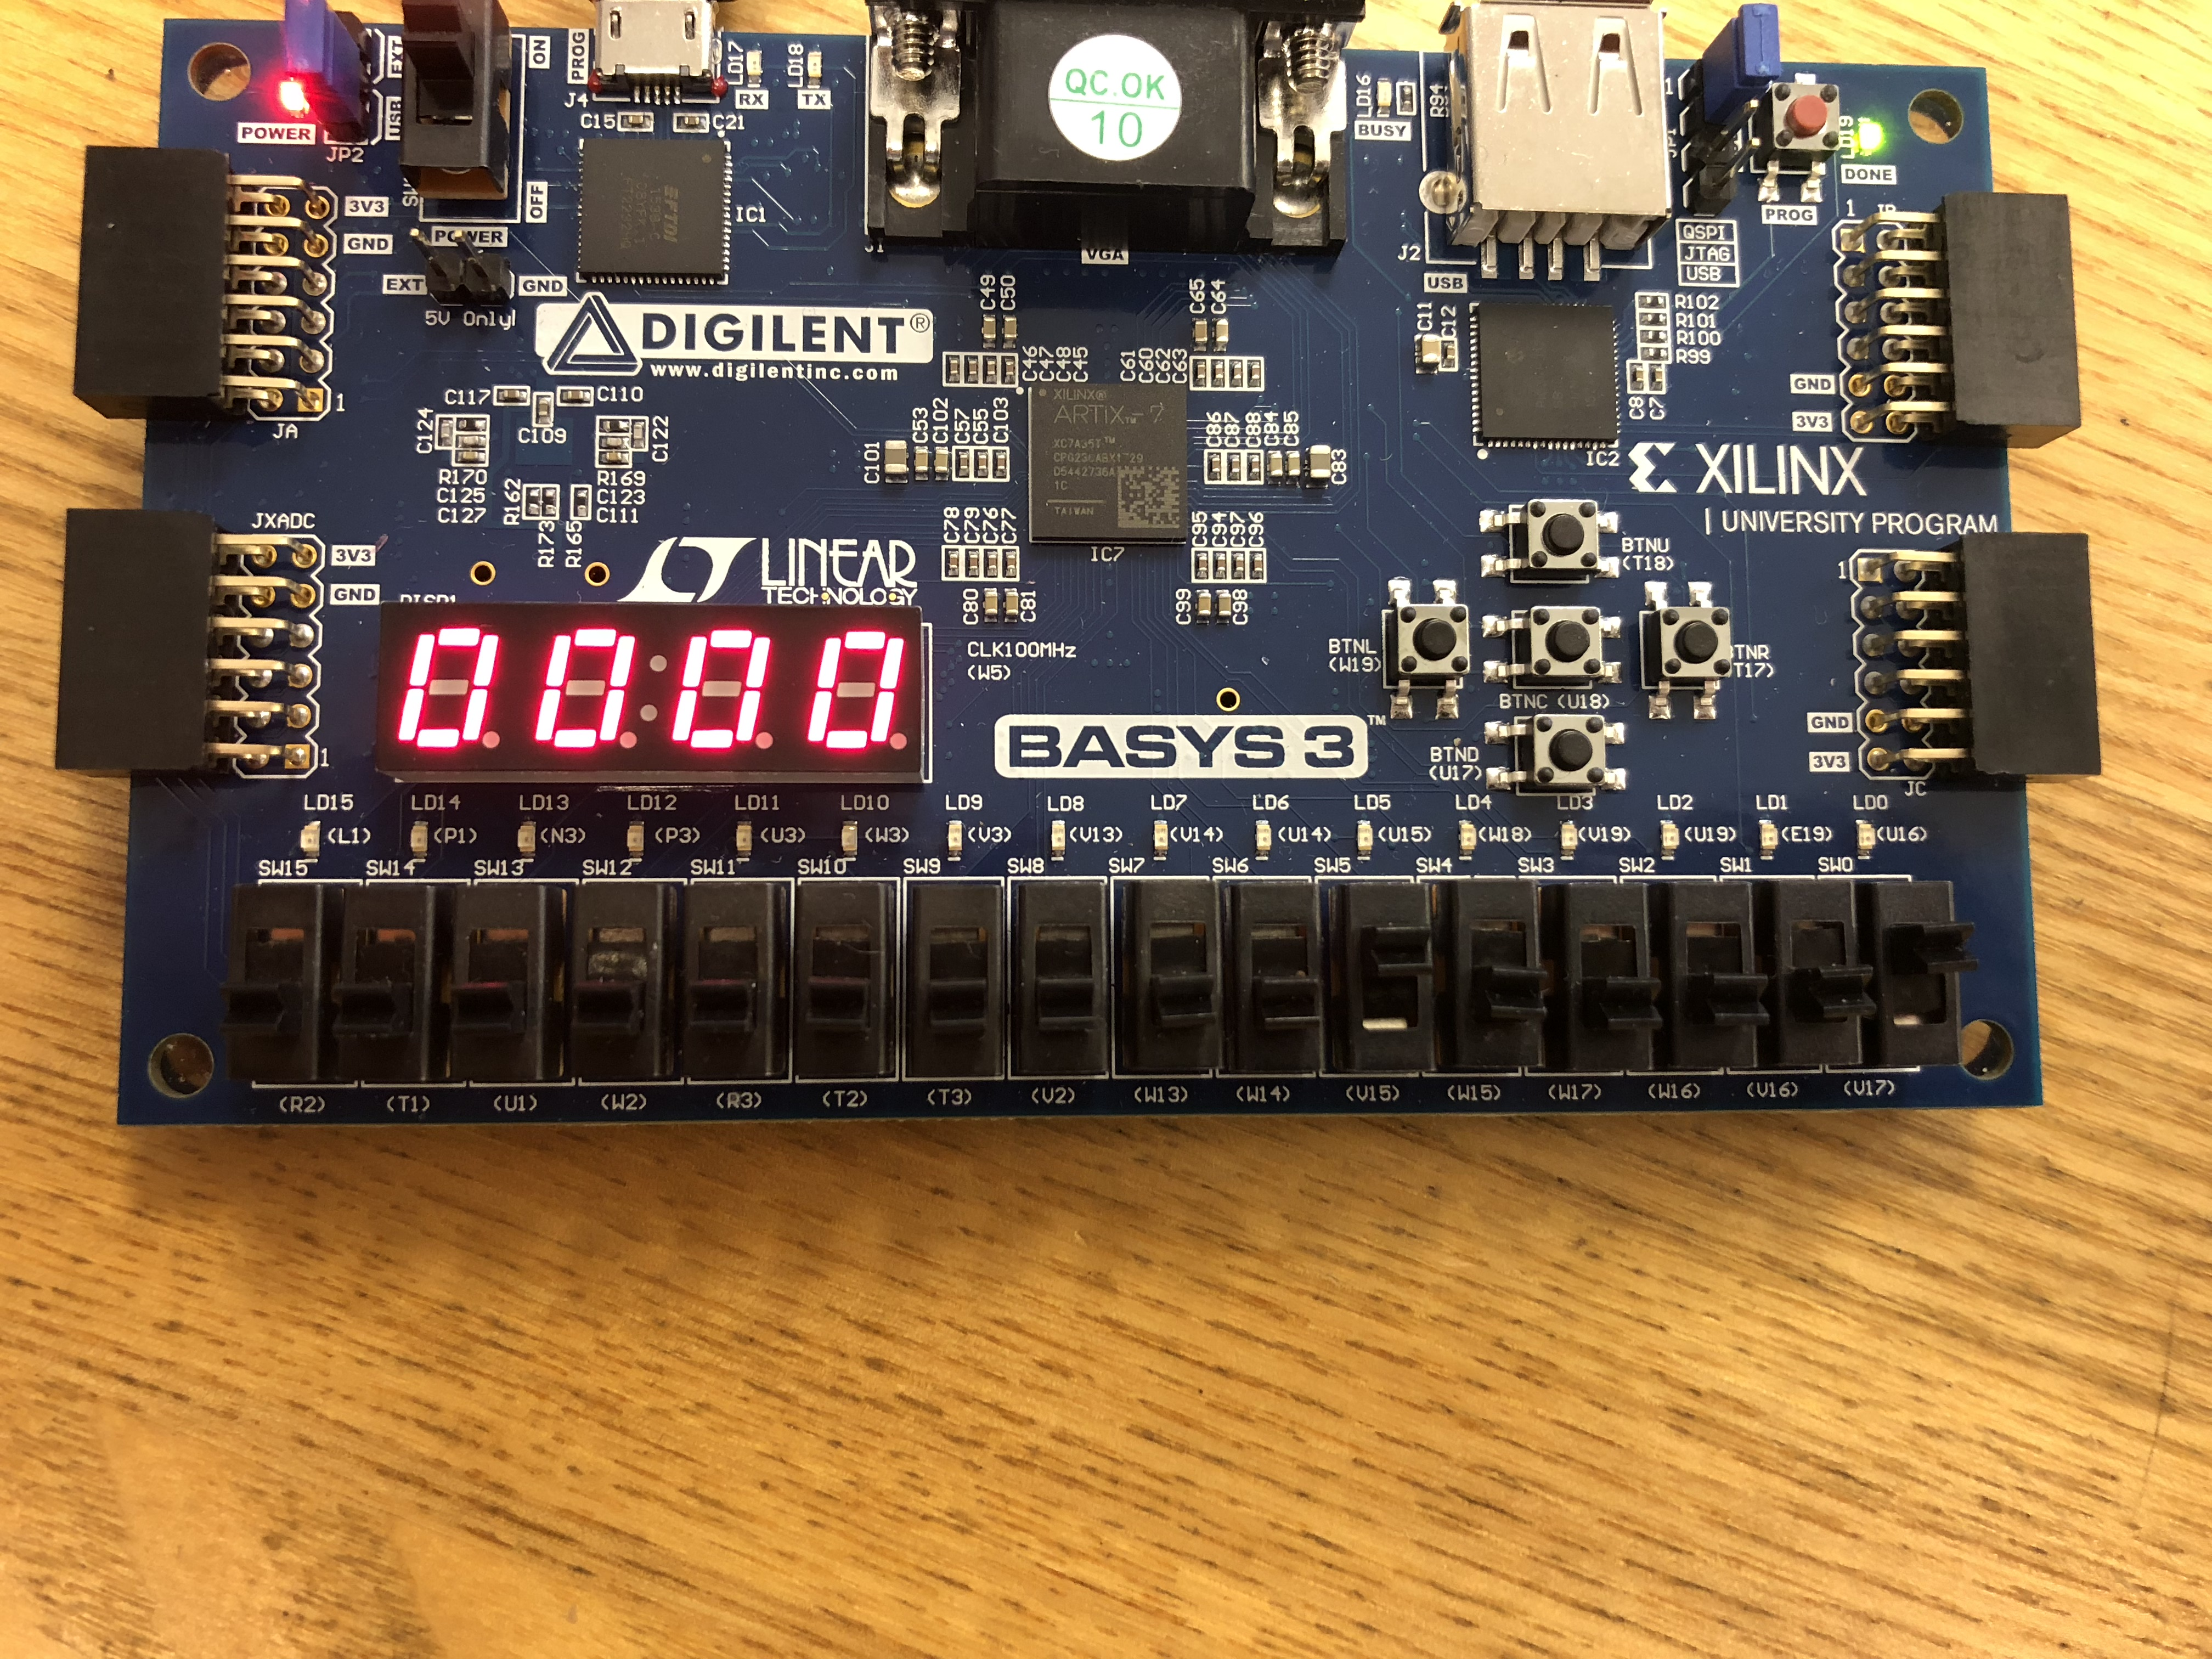
\includegraphics[width=0.5\textwidth]{../report-images/Part2/IMG_3100.jpg}
	\caption{\label{fig:p2img6}The input given by the switches is "0001", select is "10", therefore the output shown by the 7-segment display is "0".}
\end{center}
\end{figure}

\begin{figure}[H]
\begin{center}
	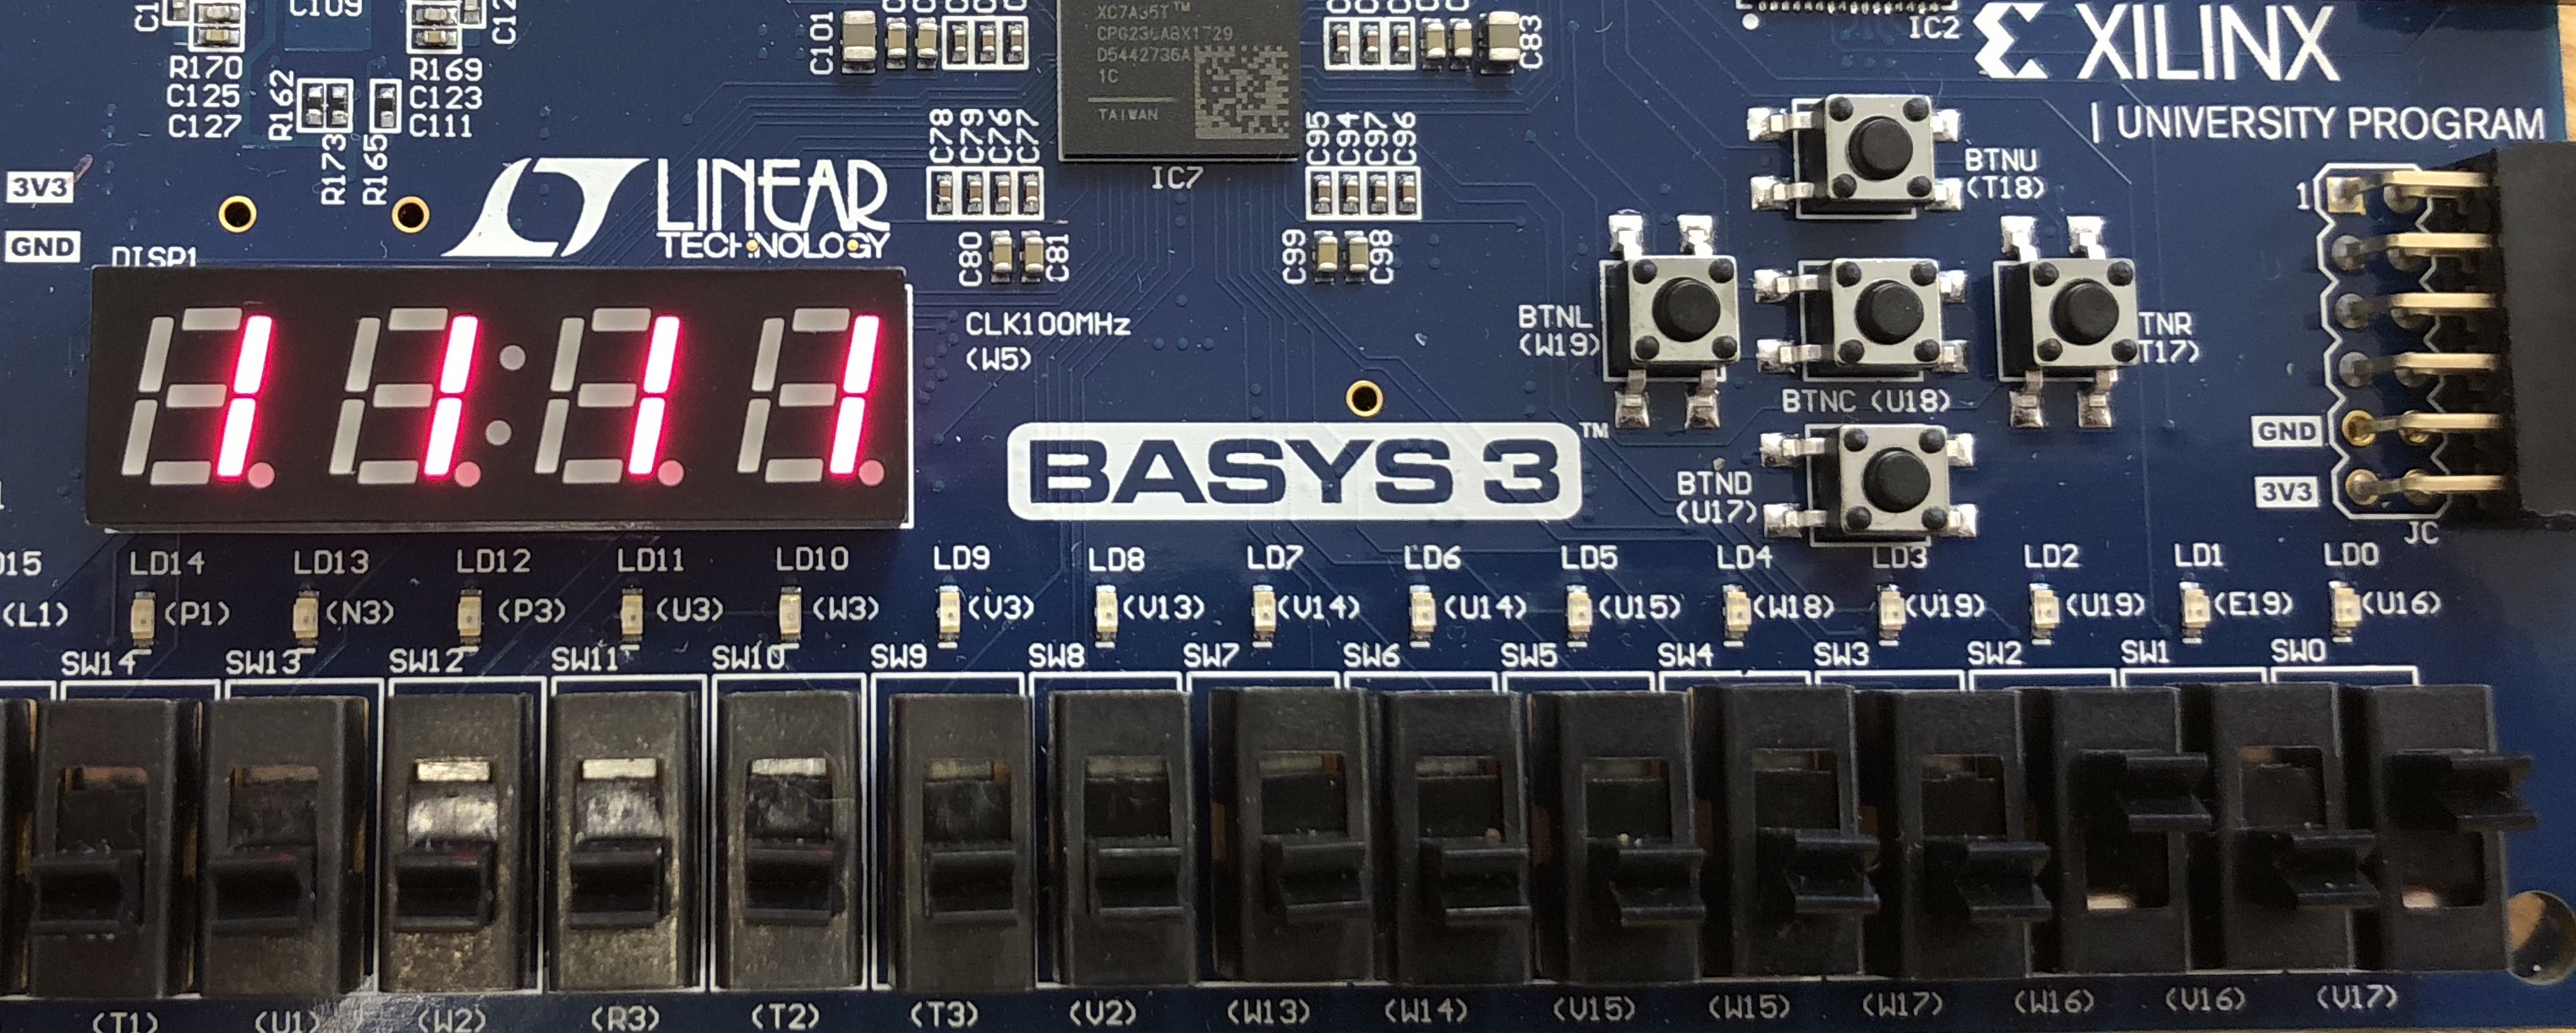
\includegraphics[width=0.5\textwidth]{../report-images/Part2/IMG_3101.jpg}
	\caption{\label{fig:p2img7}The input given by the switches is "0101", select is "00", therefore the output shown by the 7-segment display is "1".}
\end{center}
\end{figure}

\begin{figure}[H]
\begin{center}
	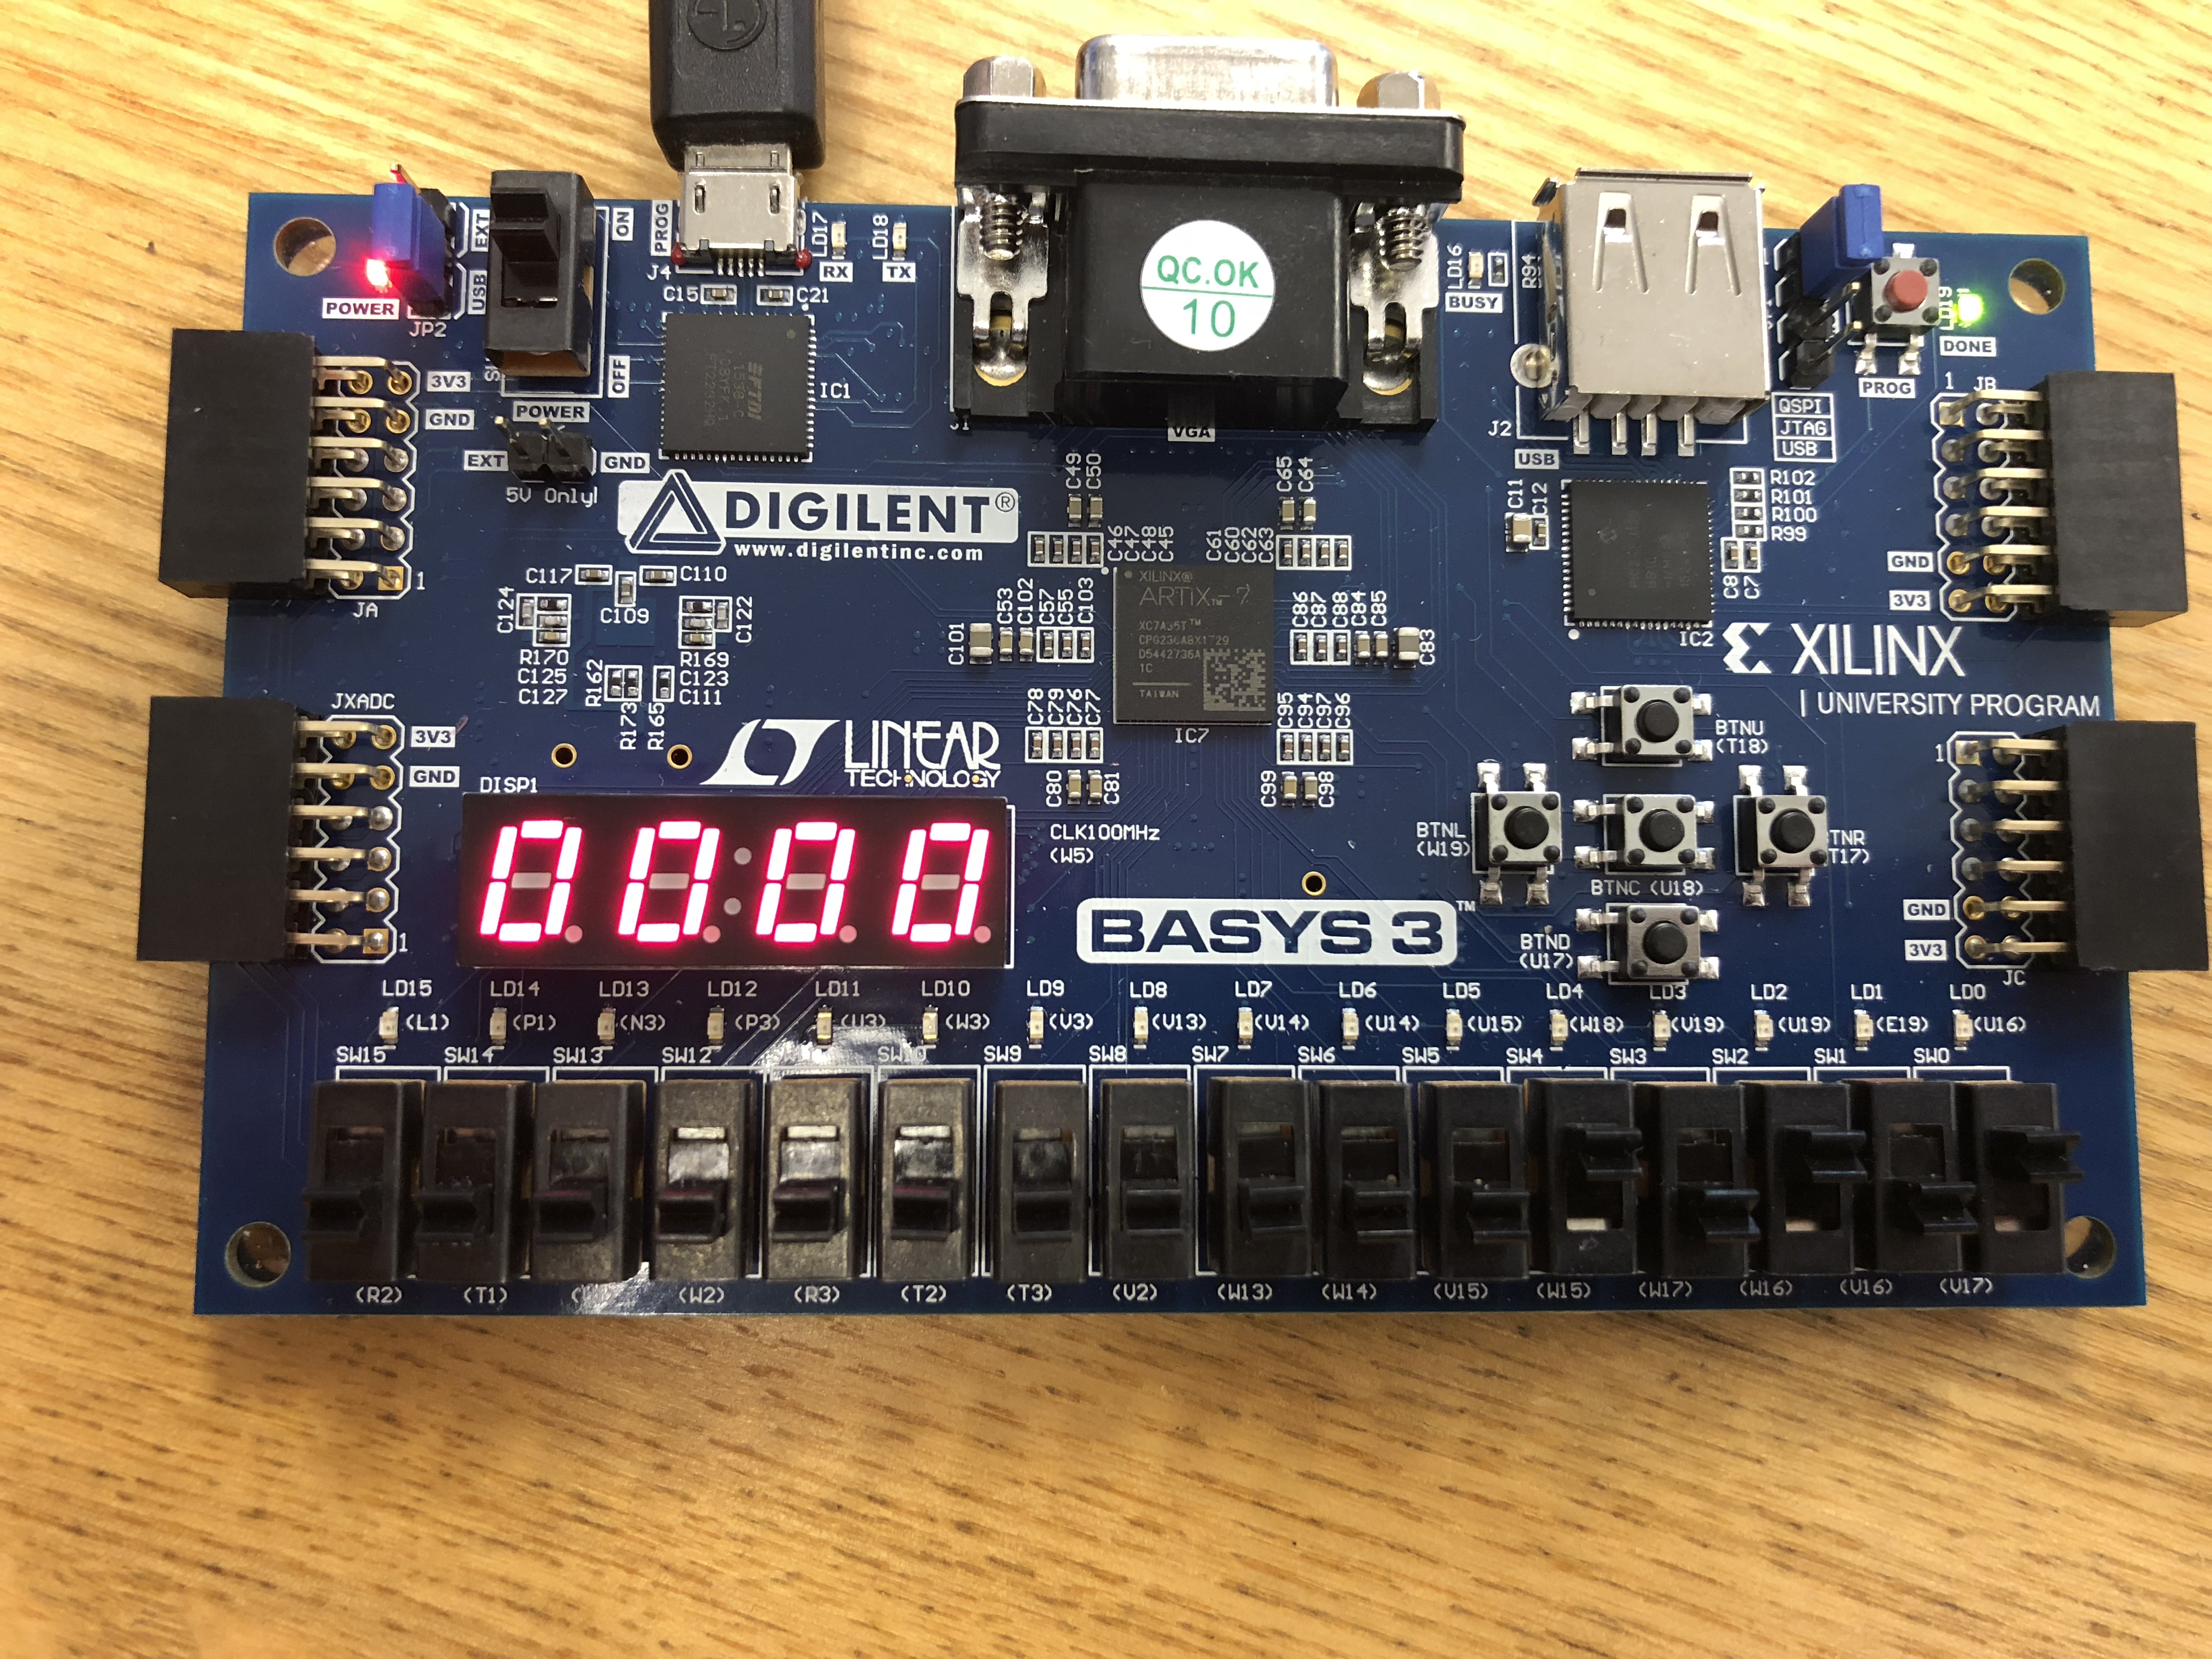
\includegraphics[width=0.5\textwidth]{../report-images/Part2/IMG_3102.jpg}
	\caption{\label{fig:p2img8}The input given by the switches is "0101", select is "01", therefore the output shown by the 7-segment display is "0".}
\end{center}
\end{figure}

\begin{figure}[H]
\begin{center}
	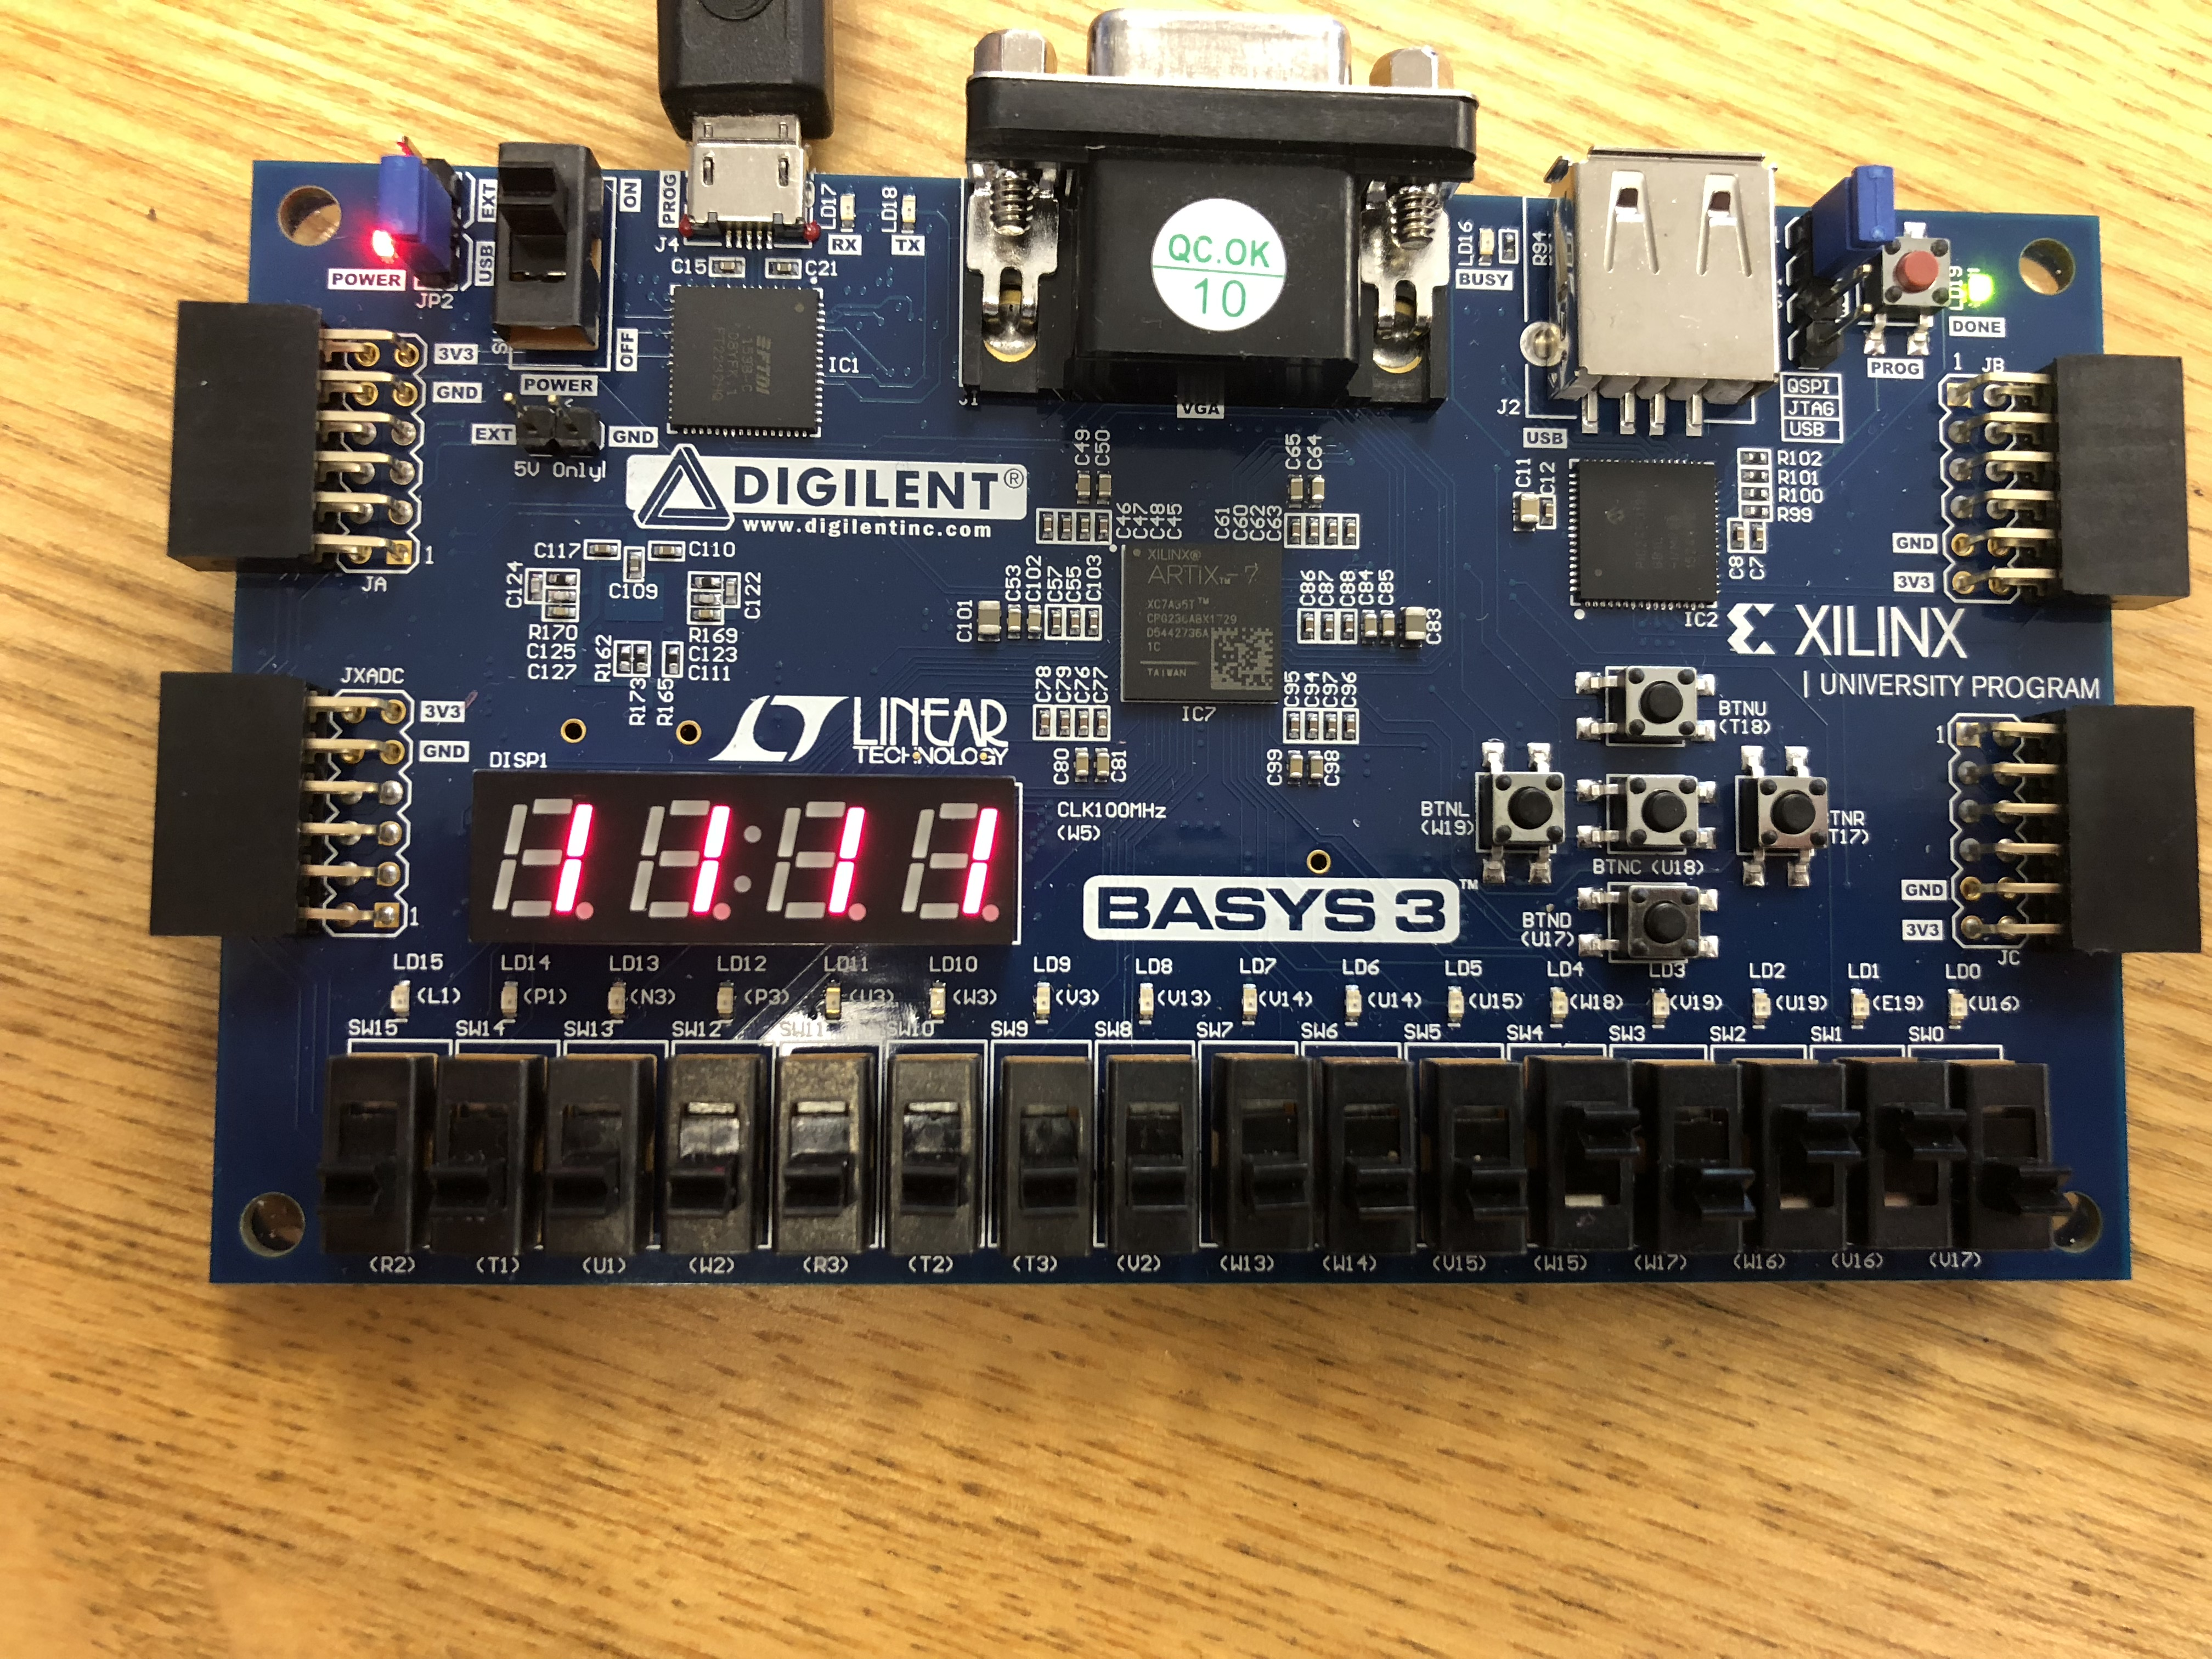
\includegraphics[width=0.5\textwidth]{../report-images/Part2/IMG_3105.jpg}
	\caption{\label{fig:p2img9}The input given by the switches is "0110", select is "01", therefore the output shown by the 7-segment display is "1".}
\end{center}
\end{figure}

\begin{figure}[H]
\begin{center}
	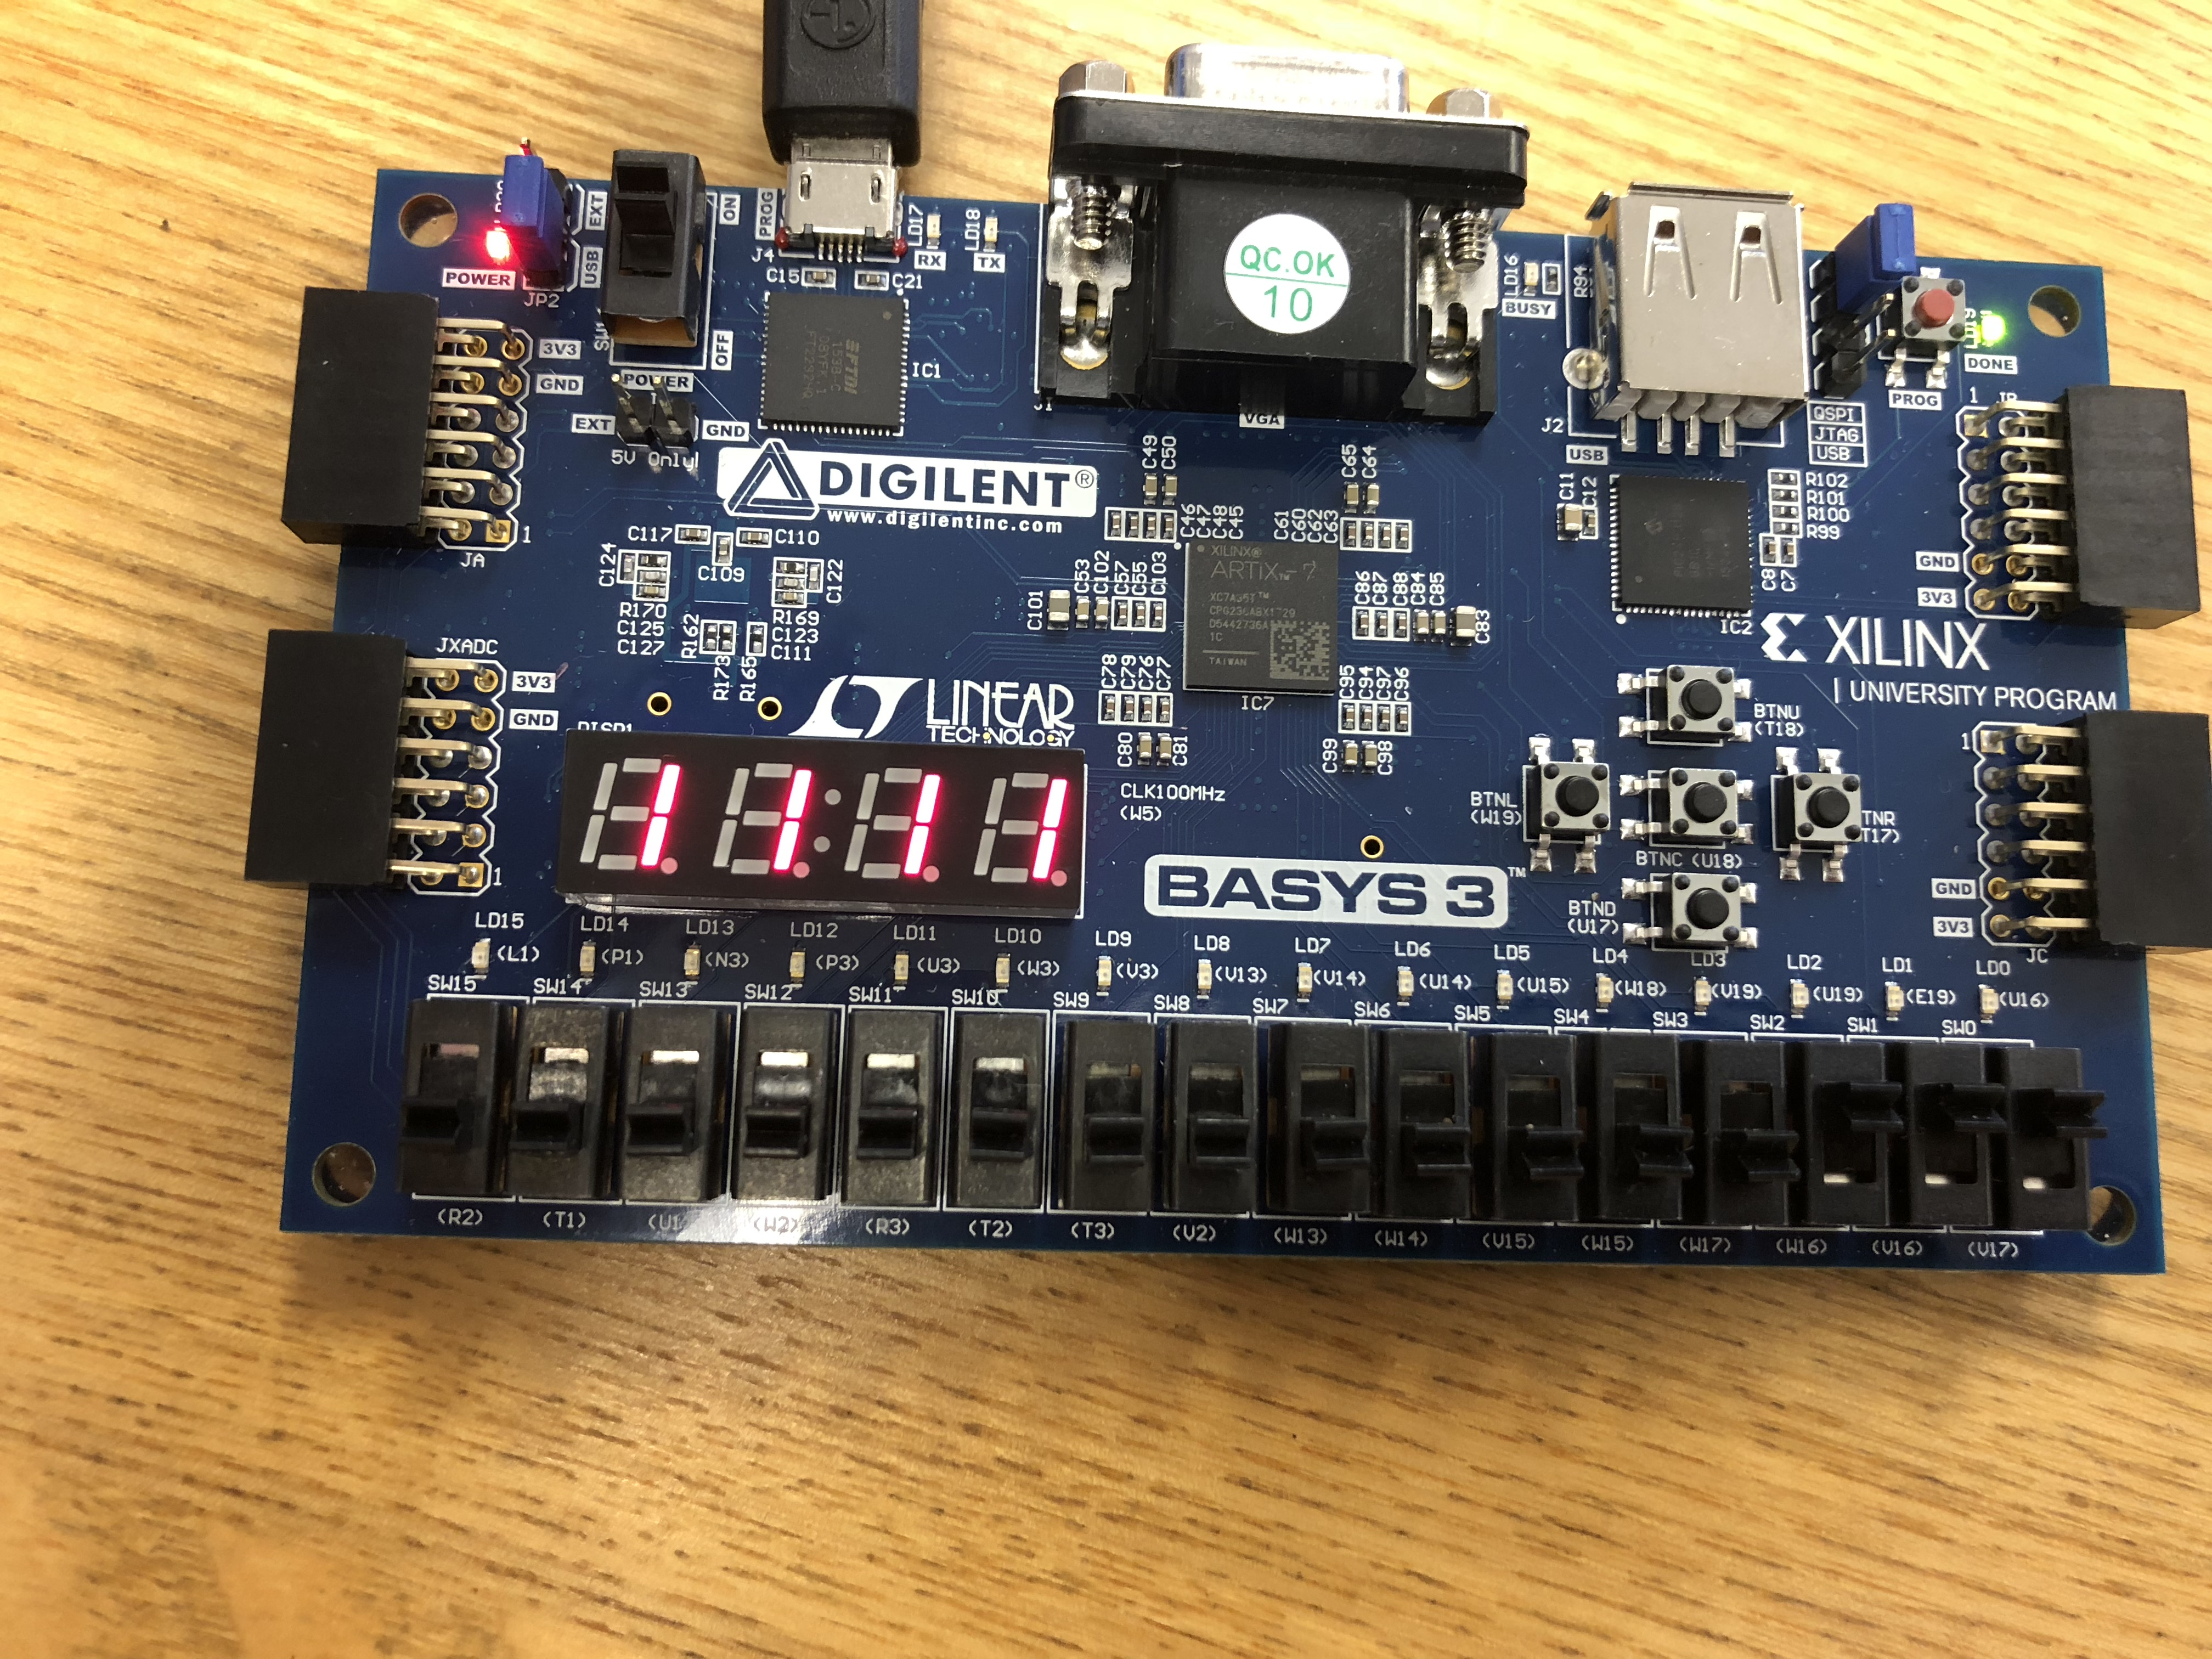
\includegraphics[width=0.5\textwidth]{../report-images/Part2/IMG_3108.jpg}
	\caption{\label{fig:p2img10}The input given by the switches is "0111", select is "00", therefore the output shown by the 7-segment display is "1".}
\end{center}
\end{figure}

\begin{figure}[H]
\begin{center}
	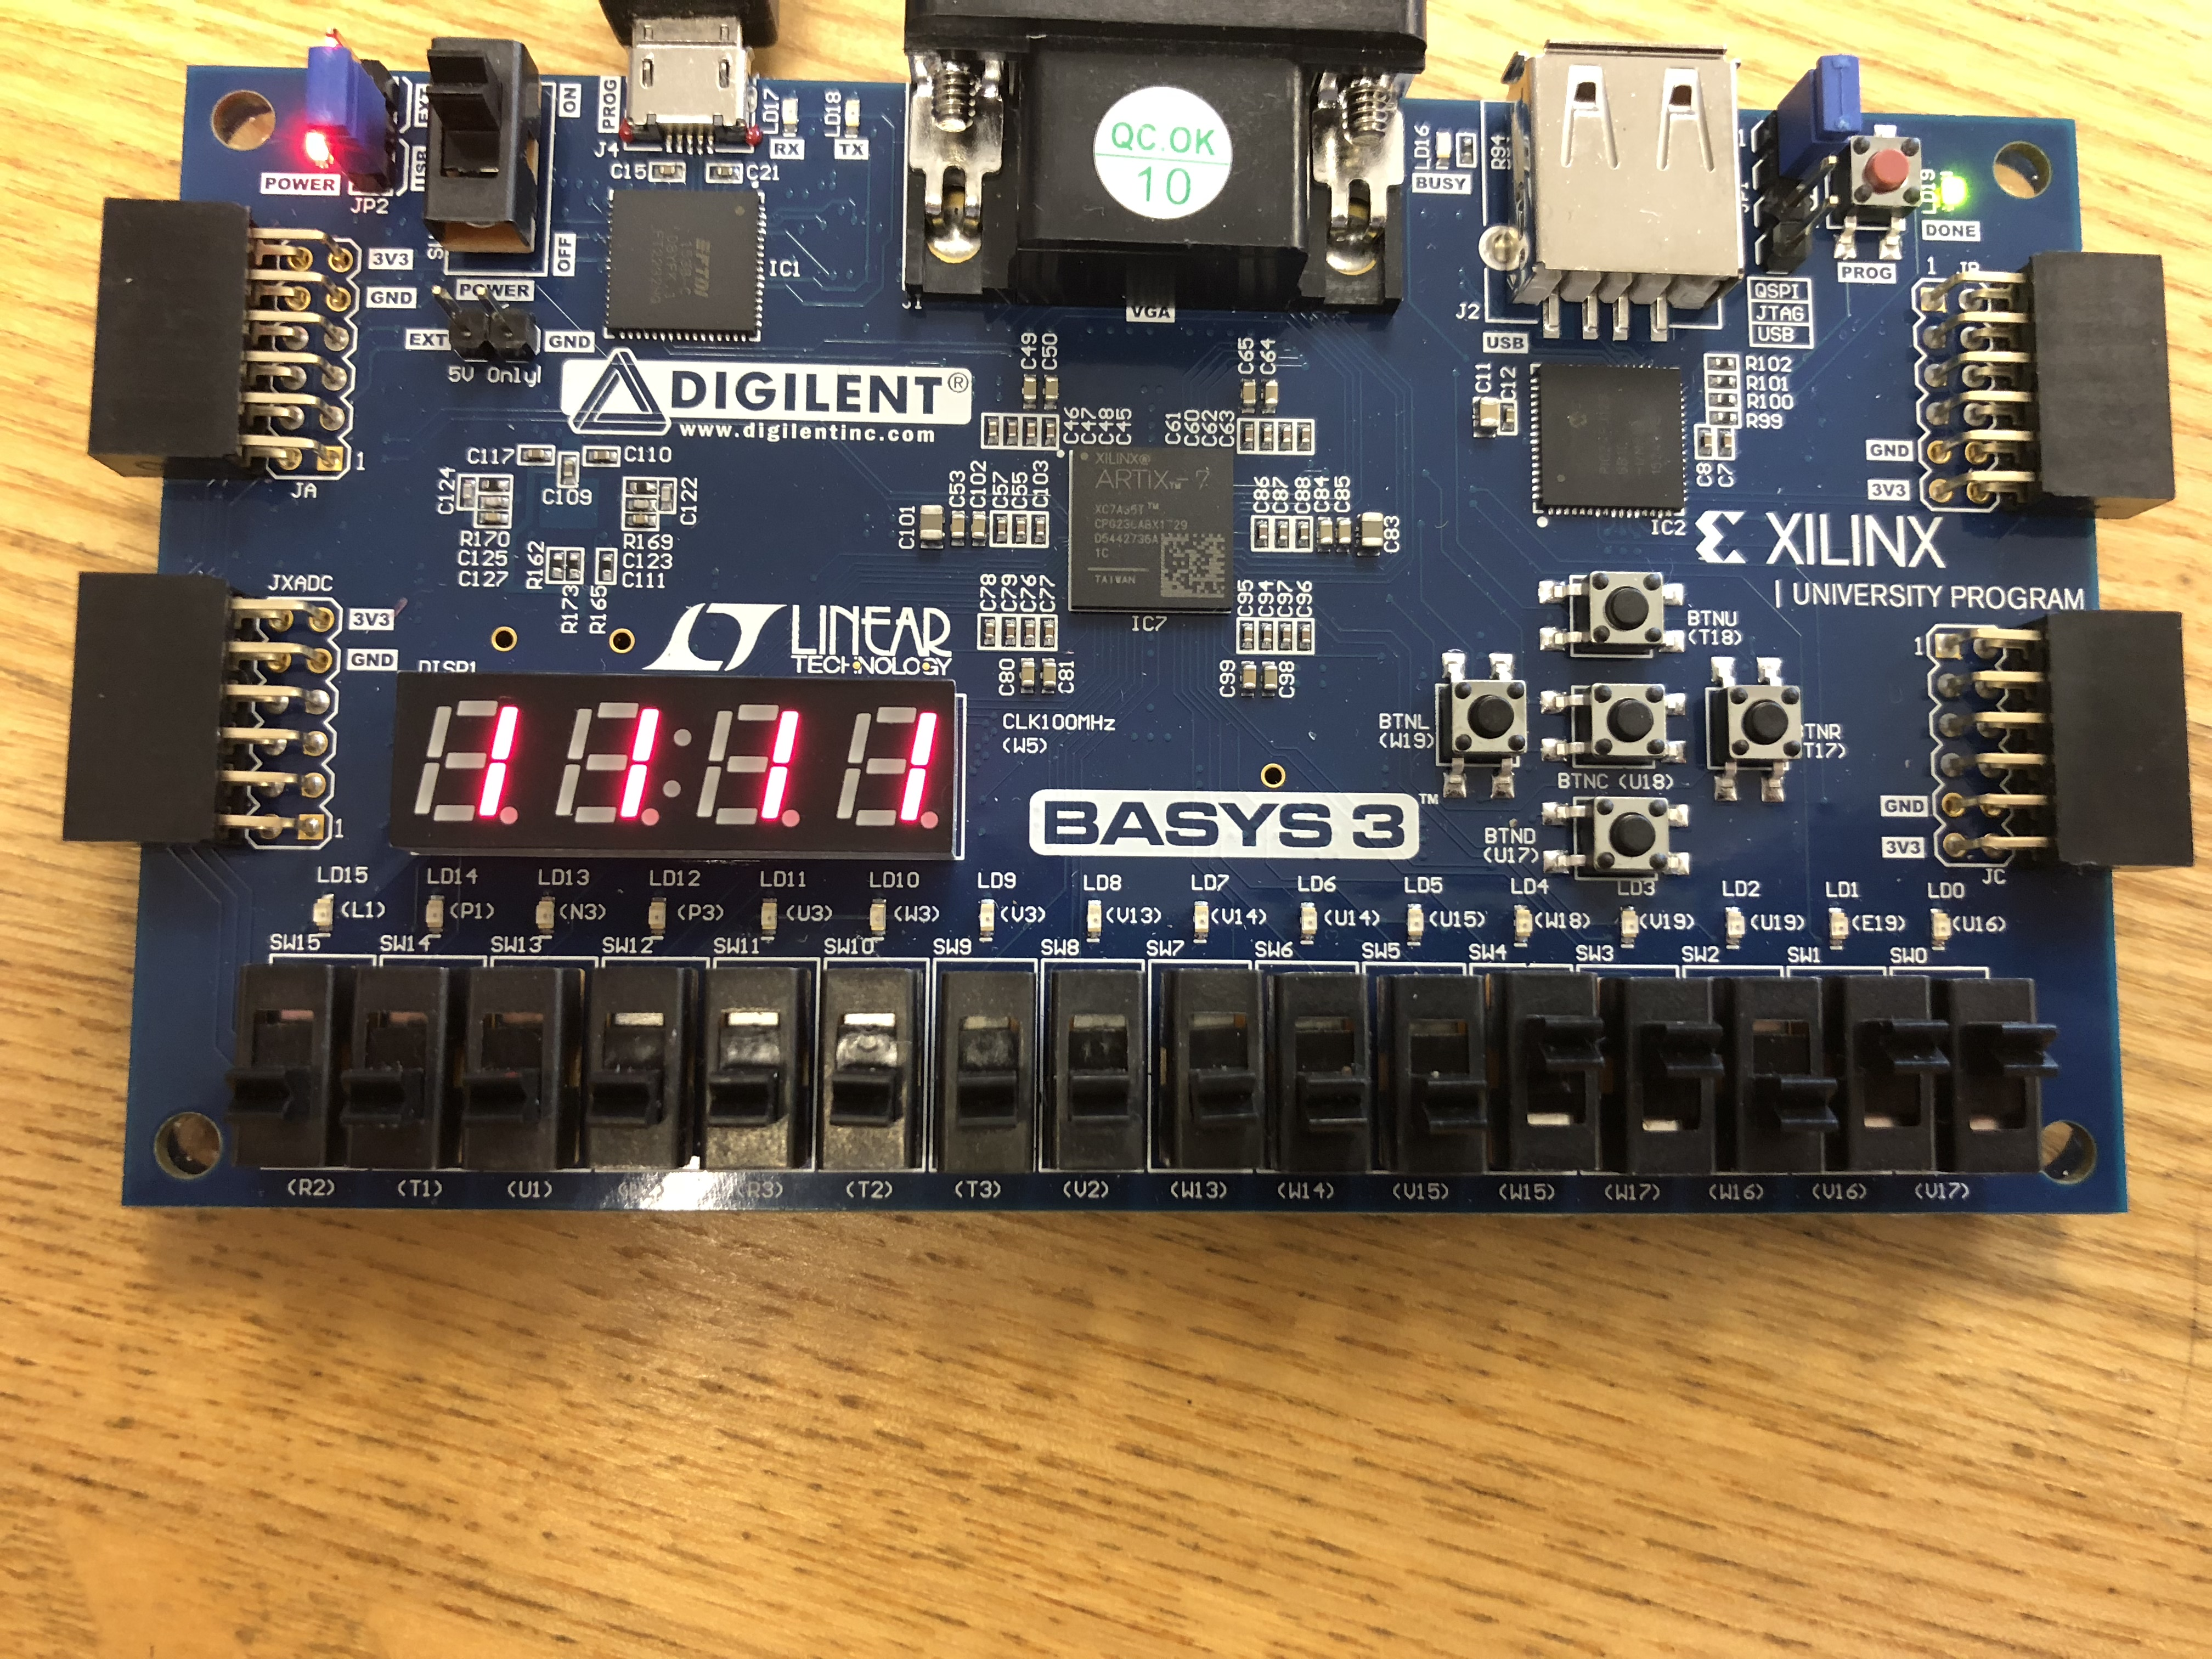
\includegraphics[width=0.5\textwidth]{../report-images/Part2/IMG_3112.jpg}
	\caption{\label{fig:p2img11}The input given by the switches is "1011", select is "01", therefore the output shown by the 7-segment display is "1".}
\end{center}
\end{figure}

\begin{figure}[H]
\begin{center}
	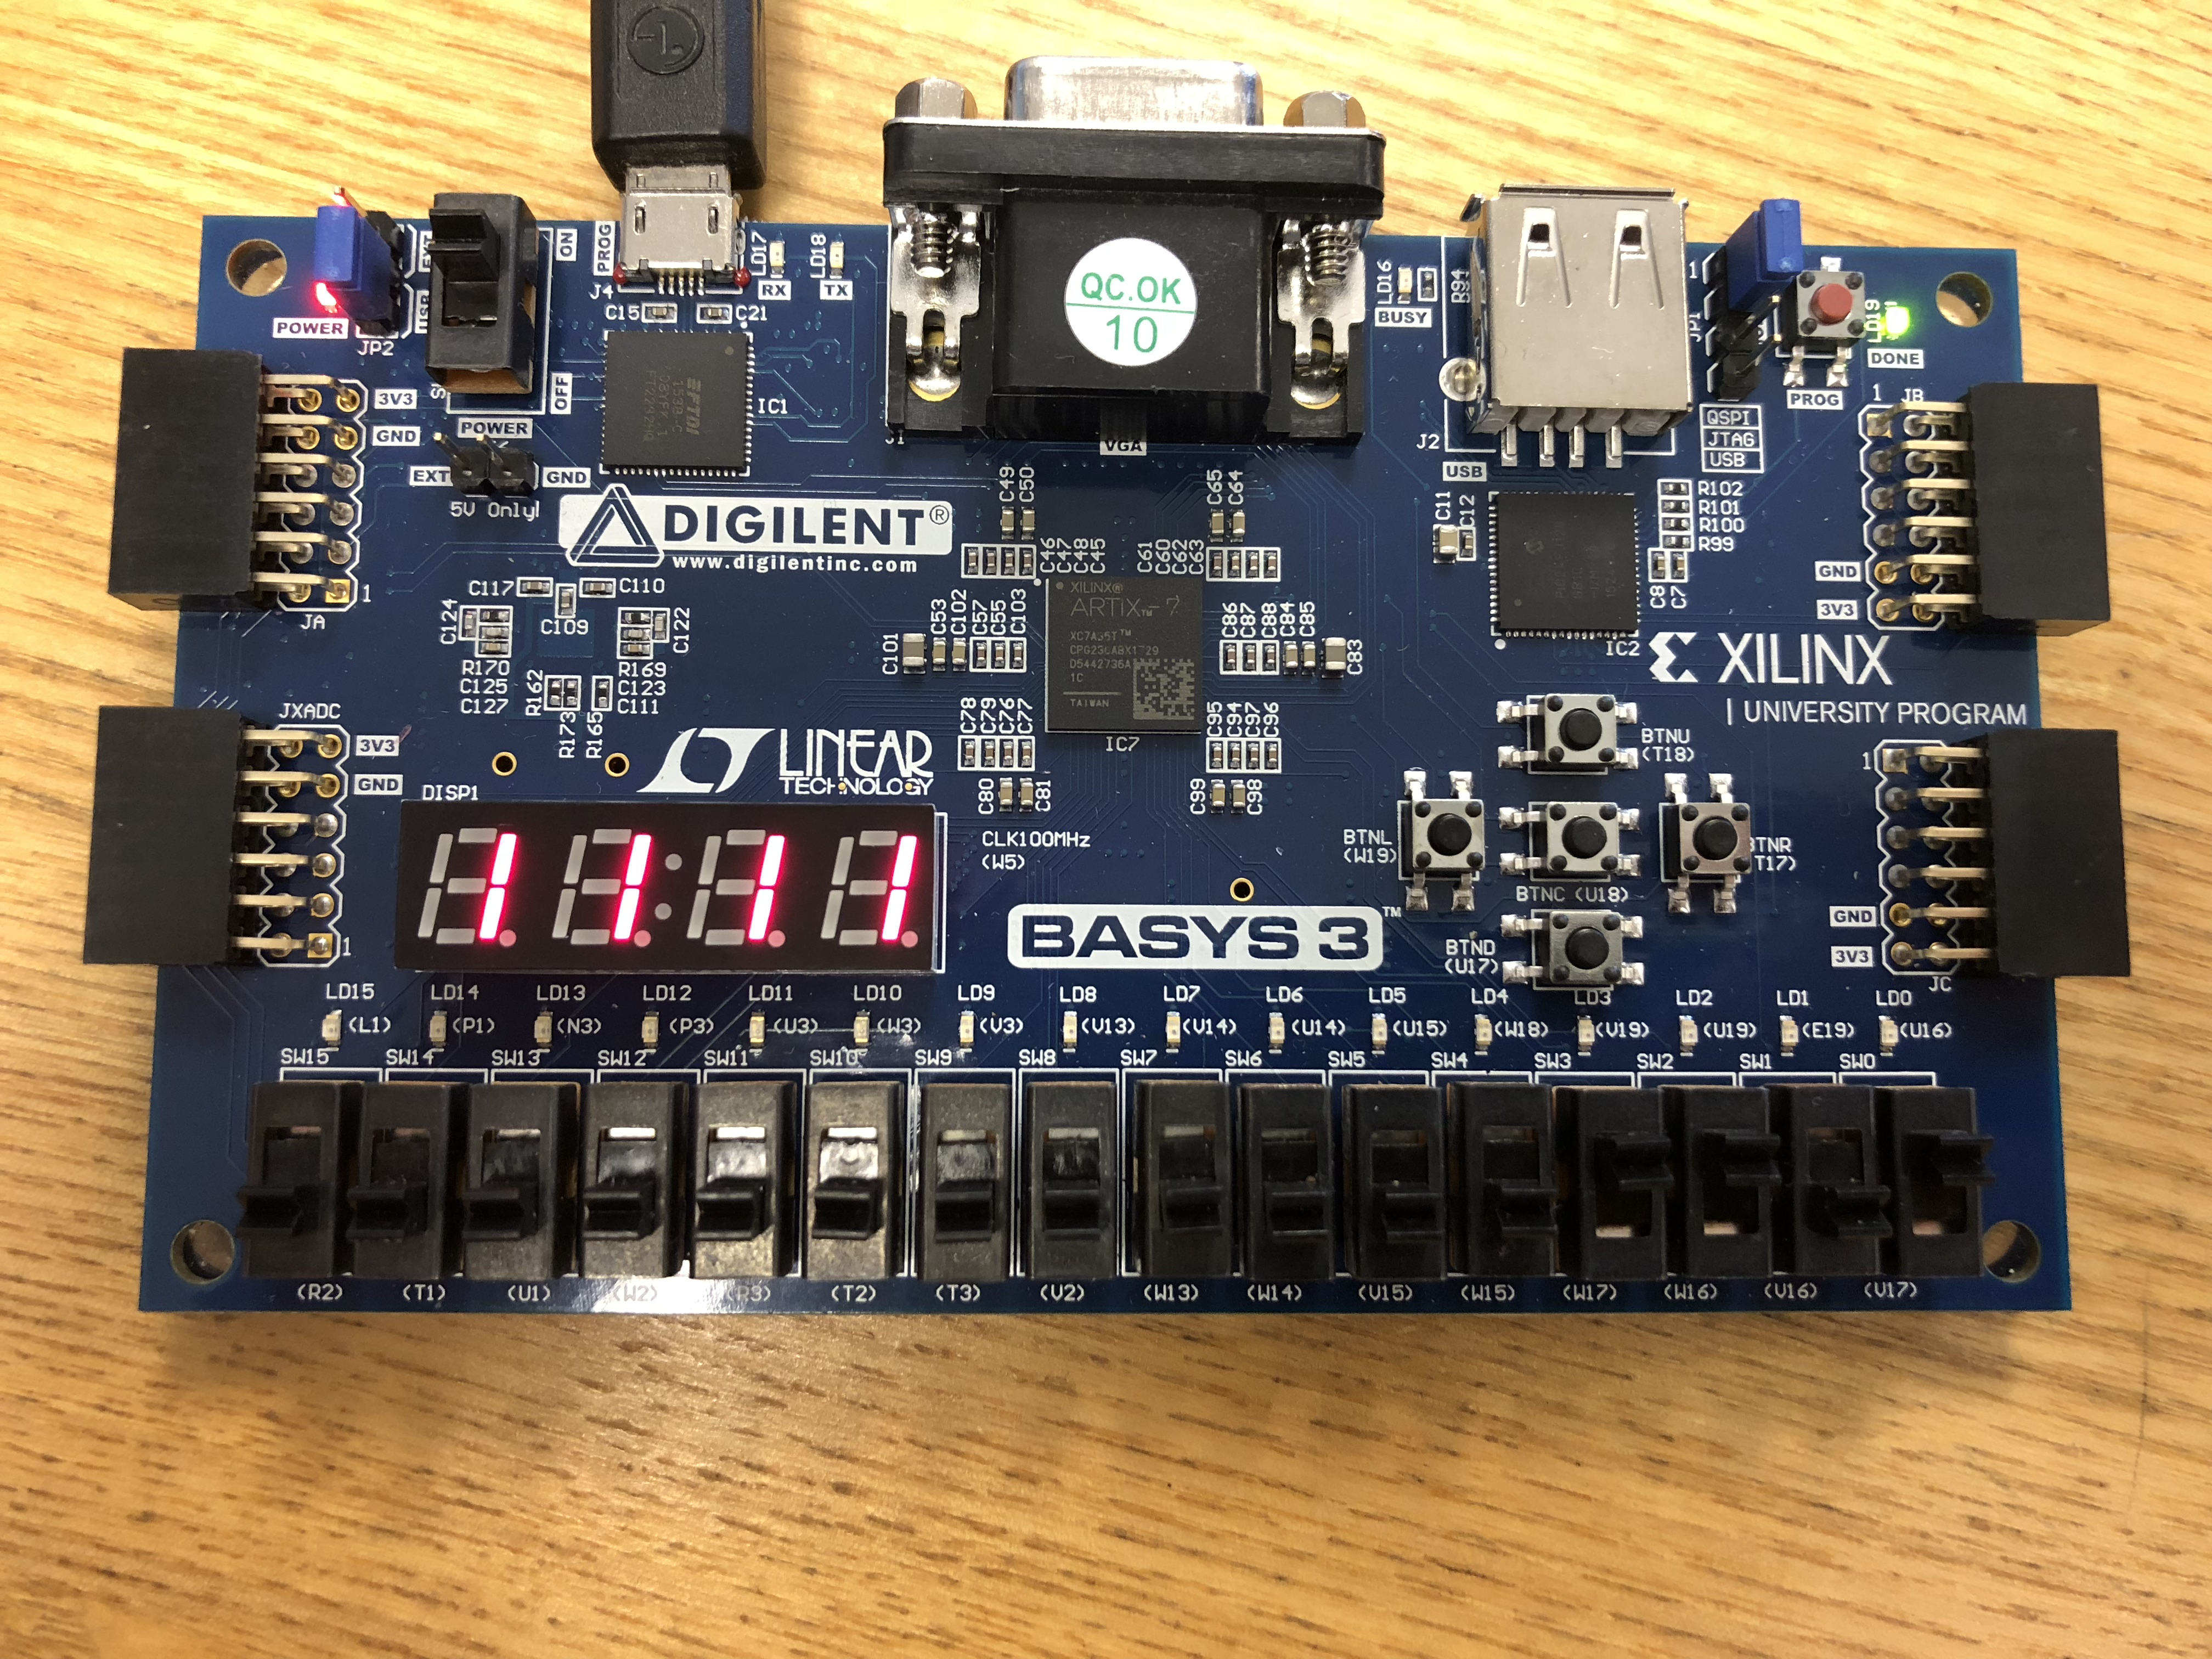
\includegraphics[width=0.5\textwidth]{../report-images/Part2/IMG_3114.jpg}
	\caption{\label{fig:p2img12}The input given by the switches is "1101", select is "00", therefore the output shown by the 7-segment display is "1".}
\end{center}
\end{figure}

\begin{figure}[H]
\begin{center}
	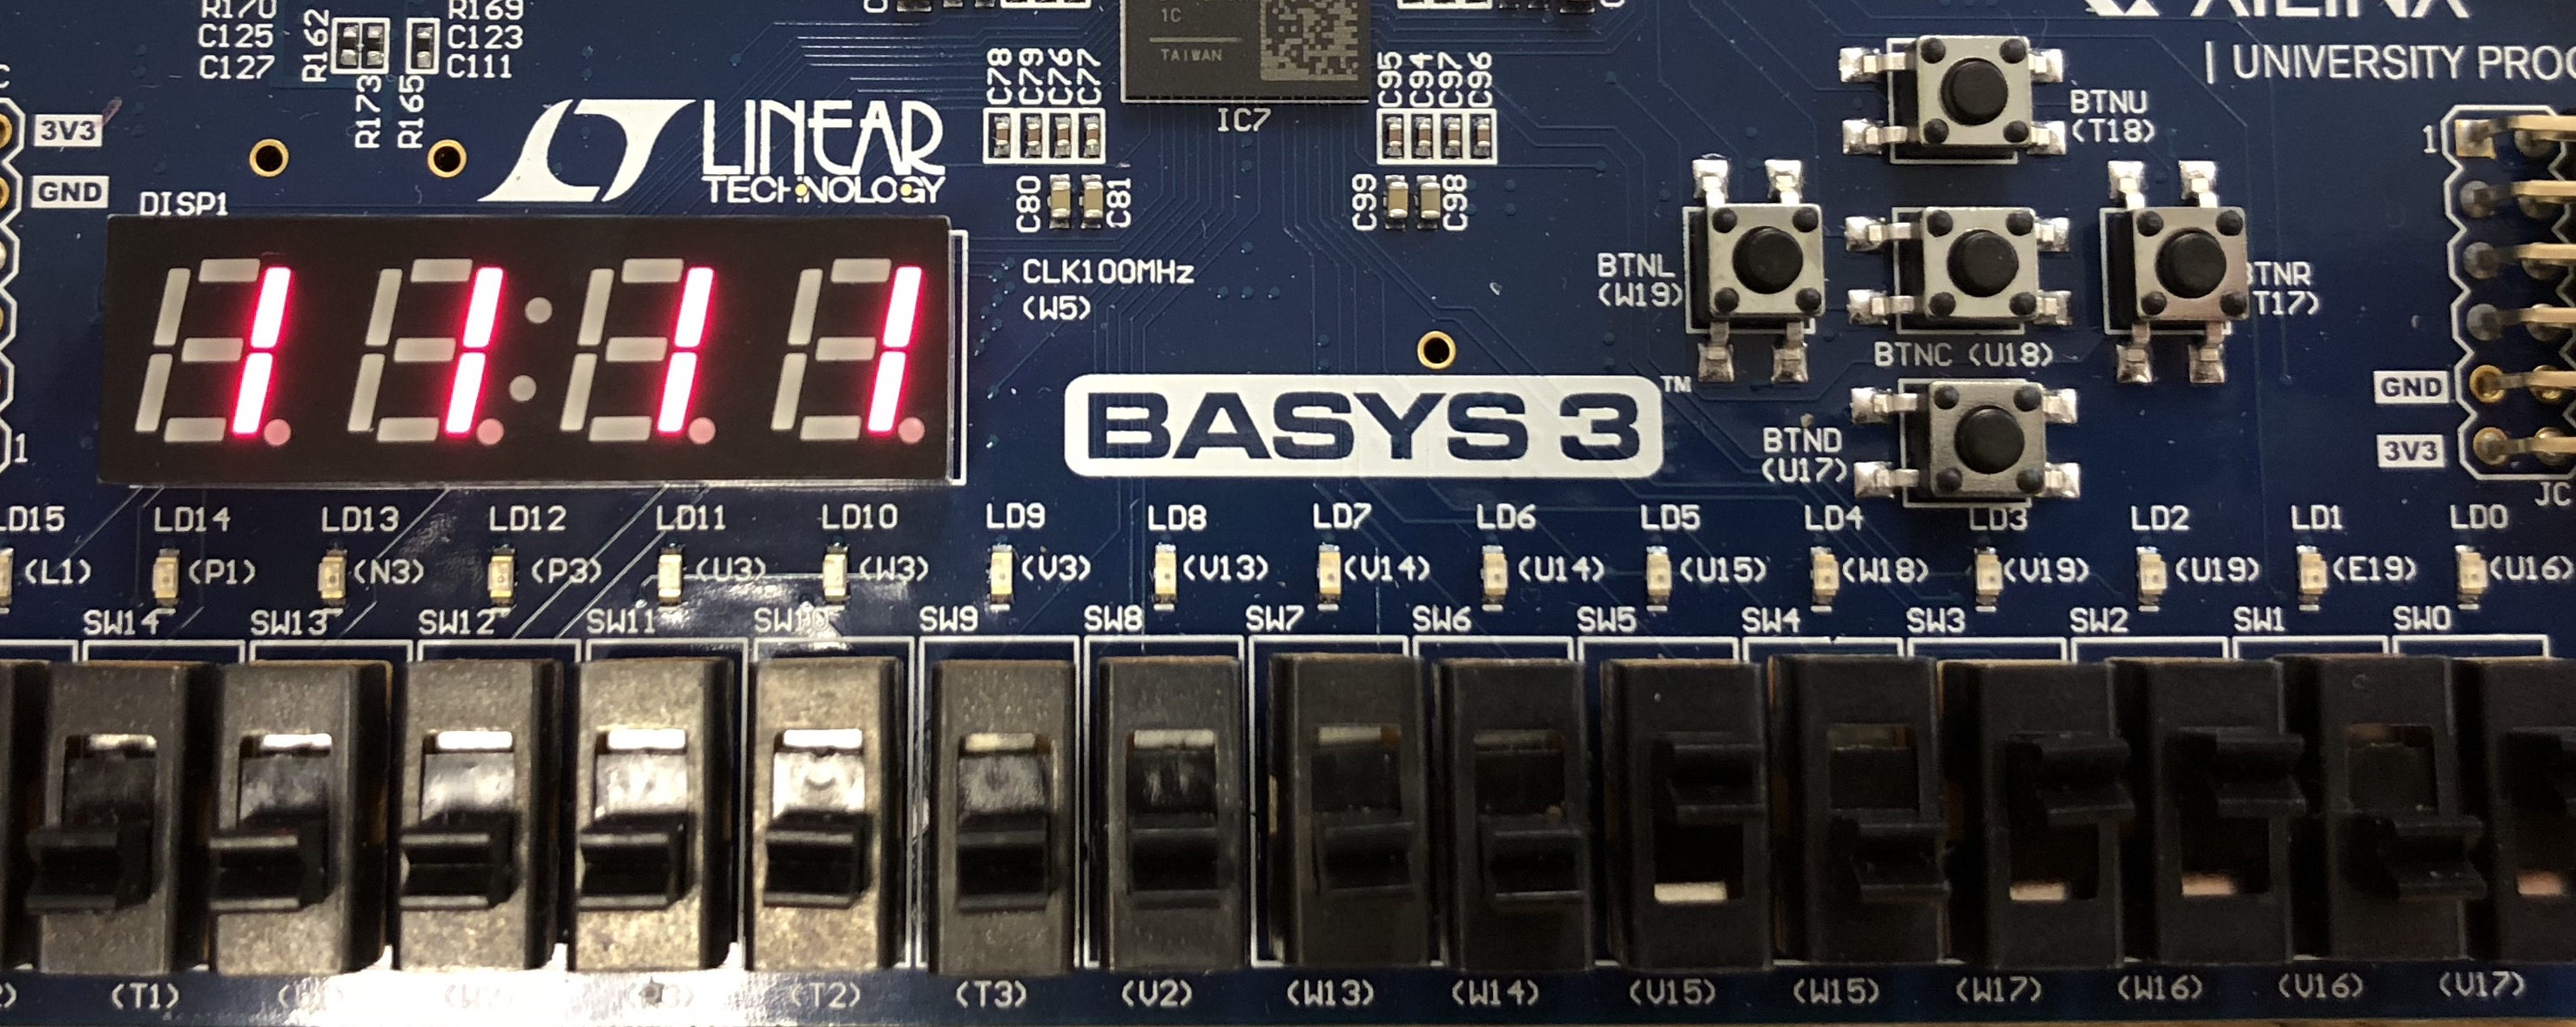
\includegraphics[width=0.5\textwidth]{../report-images/Part2/IMG_3116.jpg}
	\caption{\label{fig:p2img13}The input given by the switches is "1101", select is "10", therefore the output shown by the 7-segment display is "1".}
\end{center}
\end{figure}

\section{Conclusion}
In this lab, we were able to quickly and effectively implement each of the design challenges. As a result, we now have a firmer understanding of VHDL systems and components, as well as a new conceptual understanding of read-only memory than we previously had. The most difficult technical challenge in this lab was the design decisions around the use of the 7-segment display. Eventually, I think the design and the error case that we set up for the 7-segment display is highly functional and intuitive to the user.

\pagebreak

\textbf{Appendices}

\begin{appendices}

\section{Problem 1 VHDL Code}

\begin{lstlisting}[language=VHDL]
library IEEE;
use IEEE.STD_LOGIC_1164.ALL;

--Declares an entity that will represent
--read-only memory
entity rom is
    Port ( a : in STD_LOGIC_VECTOR(3 downto 0);
           o : out STD_LOGIC_VECTOR(2 downto 0));
end entity rom;

architecture rom_arch of rom is
    
begin
process(a)
    begin
    		--Will return a preset value for each address "a"
        case a is
            when "0000" => o <= "000";
            when "0001" => o <= "001";
            when "0010" => o <= "010";
            when "0011" => o <= "011";
            when "0100" => o <= "100";
            when "0101" => o <= "101";
            when "0110" => o <= "110";
            when "0111" => o <= "111";
            when "1000" => o <= "000";
            when "1001" => o <= "001";
            when "1010" => o <= "010";
            when "1011" => o <= "011";
            when "1100" => o <= "100";
            when "1101" => o <= "101";
            when "1110" => o <= "110";
            when "1111" => o <= "111";
        end case;
    end process;
end rom_arch;
\end{lstlisting}

\section{Problem 1 Constraints File}
\begin{figure}[H]
\begin{center}
	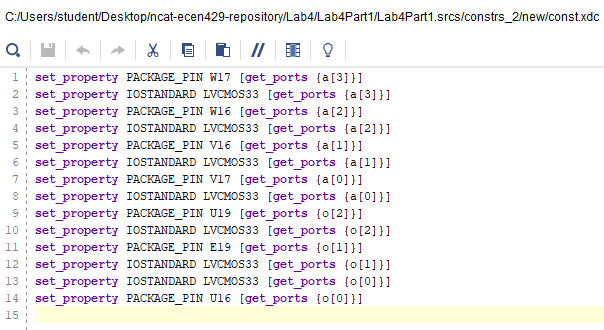
\includegraphics[width=0.5\textwidth]{../report-images/Part1Const.png}
	\caption{\label{fig:Part1ConstFile}Constraints file for Problem 1.}
\end{center}
\end{figure}

\section{Problem 2 VHDL Code}
\begin{lstlisting}[language=VHDL]
library IEEE;
use IEEE.STD_LOGIC_1164.ALL;

--Declares an entity that will represent
--read-only memory
entity rom is
    Port ( a : in STD_LOGIC_VECTOR(3 downto 0);
           o : out STD_LOGIC_VECTOR(2 downto 0));
end entity rom;

architecture rom_arch of rom is
    
begin
process(a)
    begin
    		--Will return a preset value for each address "a"
        case a is
            when "0000" => o <= "000";
            when "0001" => o <= "001";
            when "0010" => o <= "010";
            when "0011" => o <= "011";
            when "0100" => o <= "100";
            when "0101" => o <= "101";
            when "0110" => o <= "110";
            when "0111" => o <= "111";
            when "1000" => o <= "000";
            when "1001" => o <= "001";
            when "1010" => o <= "010";
            when "1011" => o <= "011";
            when "1100" => o <= "100";
            when "1101" => o <= "101";
            when "1110" => o <= "110";
            when "1111" => o <= "111";
        end case;
    end process;
end rom_arch;

library IEEE;
use IEEE.STD_LOGIC_1164.ALL;

--Declares a ROM unit whose output is read through
--a multiplexer, one bit at a time
entity rom_mux is
    Port ( x : in STD_LOGIC_VECTOR(3 downto 0);
           sel : in STD_LOGIC_VECTOR(1 downto 0);
           z : out STD_LOGIC_VECTOR(6 downto 0));
end rom_mux;

architecture Behavioral of rom_mux is
--Declares a component of the ROM entity above
component rom is port(a : in STD_LOGIC_VECTOR(3 downto 0); 
	o : out STD_LOGIC_VECTOR(2 downto 0));
end component rom;

--This is the returned ROM value at the given address
signal val : STD_LOGIC_VECTOR(2 downto 0);

begin
    rom_com : rom port map(x, val);
    process(sel)
        begin
        		--selects which bit of "val" to return
            case sel is
                when "00" => 
                    if(val(0) = '1') then z <= "1001111";
                    else z <= "0000001";
                    end if;
                when "01" =>
                    if(val(1) = '1') then z <= "1001111";
                    else z <= "0000001";
                    end if;
                when "10" => 
                    if(val(2) = '1') then z <= "1001111";
                    else z <= "0000001";
                    end if;
                when others => z <= "0000000";
            end case;
    end process;
end Behavioral;
\end{lstlisting}

\section{Problem 2 Constraints File}
\begin{figure}[H]
\begin{center}
	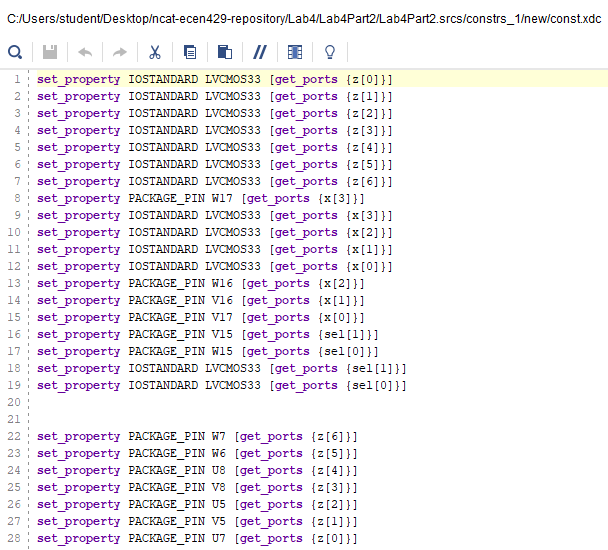
\includegraphics[width=0.5\textwidth]{../report-images/Part2Const.png}
	\caption{\label{fig:Part2ConstFile}Constraints file for Problem 2.}
\end{center}
\end{figure}

\end{appendices}
\end{document}
